% !TEX root = ../McCoy-Dissertation.tex
\chapter[Substrate-Conformal Imprint Lithography (SCIL) for Replication of X-ray Reflection Gratings]{Substrate-Conformal Imprint \\Lithography for Replication of \\X-ray Reflection Gratings}\label{ch:grating_replication} 
%%%%%%%%%%%%%%%%%%%%%%%%%%%%%%%%%%%%%%%%%-------------------------------------------------- 
The process of \emph{substrate-conformal imprint lithography (SCIL)} \cite{Verschuuren10} is introduced in \cref{sec:ch1_conclusions} as a method for high-throughput replication of x-ray reflection gratings, which is essential for achieving a sufficient collecting area for spectroscopy, $A_{\text{col}}$, in future instruments that call for large numbers of grating replicas such as the \emph{XGS} for the \emph{Lynx} mission concept \cite[\emph{cf.\@} \cref{sec:astro_plasmas,sec:grating_tech_dev}]{Gaskin19,McEntaffer19}. 
Unlike rigid-stamp nanoimprint processes such as UV-NIL \cite[\emph{cf.\@} \cref{sec:nanoimprint}]{Chou96,Haisma96,Schift08,Schift10}, SCIL centers on the use of a low-cost, flexible stamp that is molded from a master template, which in this context, defines a grating surface relief \cite{Verschuuren10,Verschuuren17,Verschuuren19}. 
This lithographic approach enables nanoscale patterns to be imprinted in resist over large areas with a stamp that conforms locally to particulate contaminants and globally to any slight bow of the replica substrate so as to avoid damage to the master template by eliminating the need for an applied high pressure. 
Additionally, wave-like sequential imprinting made possible by the flexibility of the stamp and specialized pneumatic tooling serves to eliminate large trapped air pockets. 
For these reasons, SCIL is an attractive technique for imprinting surface reliefs for x-ray reflection gratings, which are often patterned on \SI{150}{\mm}-diameter wafers [\emph{cf.\@} \cref{sec:grating_fab_intro}]. 

Although SCIL stamps are compatible with many UV-curable, organic resists similar to those used for UV-NIL \cite{Ji10,Schift10}, high-volume production that relies on long stamp lifetime is best suited for use with a brand of inorganic resist, synthesized by \textsc{Philips SCIL Nanoimprint Solutions} \cite{philis_scil} (referred to as \textsc{Philips} hereafter) and known commercially as \textsc{NanoGlass}, which cures through a thermodynamically-driven, silica \emph{sol-gel process} \cite{Verschuuren10,Verschuuren17}. 
Packaged equipment that automates sol-gel resist spin-coating and the pneumatic-based SCIL wafer-scale imprint method for high-volume replication has also been developed by \textsc{Philips} \cite{philis_scil}. 
Using this production platform, known as \textsc{AutoSCIL}, a single composite stamp is capable of producing $\gtrapprox \num{700}$ imprints in \textsc{NanoGlass} resist at a rate of \num{60}, \SI{150}{\mm}-diameter wafers per hour without pattern degradation \cite{Verschuuren17,Verschuuren18,Verschuuren19}. 
This technique was first applied to x-ray reflection grating technology for the development of \emph{WRXR} \cite{Miles17,Miles18b,Tutt19}, which utilized \textsc{AutoSCIL} to produce \num{26} replicas of a \SI{110}{\cm\squared} master grating fabricated via electron-beam lithography (EBL) and crystallographic etching in a manner similar to what is described in \cref{sec:crystal_etching} \cite{Miles19,Verschuuren18}. 
While this relatively low imprint throughput can, in principle, be achieved by other means, future instruments such as \emph{tREXS}, \emph{OGRE} and the \emph{XGS} \cite{Miles19b,Tutt18,McEntaffer19}, which each require many more grating replicas, are expected to benefit from the capabilities of \textsc{AutoSCIL}. 

The application of SCIL to grating replication technology was motivated by an initial set of experiments, carried out in collaboration with \textsc{Philips}, that characterize the quality of imprints produced from a master grating template wet-etched in silicon \cite{McCoy17}, which was fabricated by staff at Penn State Nanofabrication Laboratory \cite[\emph{cf.\@} \cref{sec:crystal_etching}]{Miles18,PSU_MRI_nanofab}. 
These experiments and related studies are the subject of this chapter, with a special focus on the impact that resist shrinkage has on blaze angle in imprinted gratings.\footnote{Supported by a NASA Space Technology Research Fellowship lasting from 2015 to 2019, much of this research is published in a peer-reviewed article \cite{McCoy20b}. In addition to the Penn State Materials Research Institute, resources of the Quattrone Nanofabrication Facility at the Singh Center for Nanotechnology \cite{Quattrone} (U.\ of Pennsylvania) were used for SCIL process development carried out in 2017 and 2018 \cite{McCoy17}.} 
First, \cref{sec:grating_fab} outlines a SCIL process for x-ray reflection grating manufacture along with the expected level of shrinkage that occurs in \textsc{NanoGlass} as the silica sol-gel network densifies with a post-imprint thermal treatment. 
Soft x-ray diffraction-efficiency measurements of an imprinted grating and its corresponding master template are then presented in \cref{sec:beamline_testing}. 
These results are analyzed in \cref{sec:discussion_scil} through a comparison of the experimental data to theoretical models for diffraction efficiency from \cref{sec:integral_method} in order to demonstrate a non-negligible level of blaze angle reduction due to resist shrinkage. 
Finally, \cref{sec:conclusion} provides conclusions and a summary for this chapter. 

\section{Grating Fabrication by SCIL}\label{sec:grating_fab}
%%%%%%%%%%%%%%%%%%%%%%%%%%%%%%%%%%%%%%%%%-------------------------------------------------- 
Regardless of the resist used for imprinting, the SCIL process relies on having stamp features carried in a material that is flexible enough for surface-conformal imprinting but stiff enough to maintain a high-fidelity stamp topography at sub-\si{\um} size scales \cite{Verschuuren10,Verschuuren17,Verschuuren19}. 
\begin{figure}
 \centering
 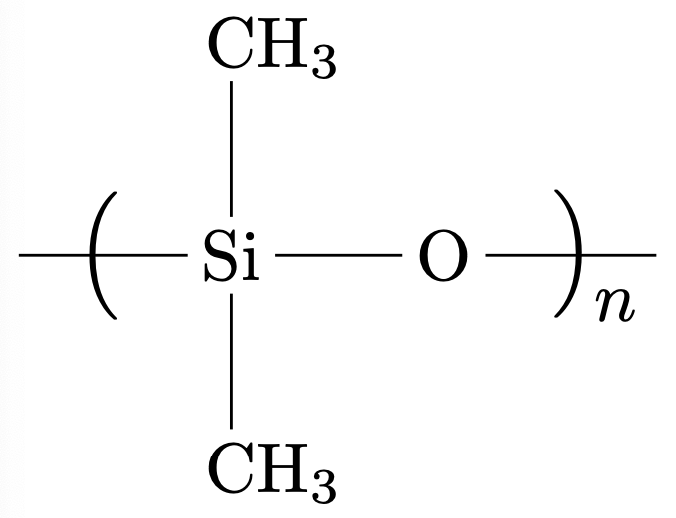
\includegraphics[scale=0.45]{Chapter-4/Figures/PDMS.png}
 \caption[Structural formula of polydimethylsiloxane (PDMS).]{Structural formula of the elastomer polydimethylsiloxane (PDMS), where siloxanes connect at the sites marked by brackets to form a longer polymer chain with side methyl groups.}\label{fig:PDMS}
 \end{figure}
A common stamp material in \emph{soft lithography} \cite{Xia98,Qin10} is \emph{polydimethylsiloxane} (PDMS), a type of \emph{elastomer} composed of many repeating units of the monomer \emph{dimethylsiloxane} (\ce{C2H6OSi}), where linear siloxanes (\emph{i.e.}, \ce{-Si-O-}) connect at the sites marked by brackets while methyl groups (\emph{i.e.}, \ce{-CH3}) terminate the remaining bonding sites of silicon \cite[\emph{cf.\@} \cref{fig:PDMS}]{Zaman19}. %as shown in \cref{fig:PDMS}, %valence-electron
With a \emph{Young's modulus}\footnote{This quantity is defined as the ratio of tensile stress to tensile strain, which essentially characterizes the stiffness of a material \cite{landau1986theory}.} on the order of \SI{1}{\mega\pascal}, however, sub-\si{\um} features in a PDMS stamp are subject to collapse and additionally, deformation of sharp corners due to surface tension \cite{Bietsch00,Hui02,Verschuuren10}. 
To circumvent this issue, modified versions of PDMS have been synthesized to have a Young's modulus that is high enough for smaller-scale imprinting but still much smaller than \SI{1}{\giga\pascal} so as to enable conformal contact over large areas. 
An example of such a material is \emph{hard-PDMS (H-PDMS)}, which features silicon-ethyl bonds (\emph{i.e.}, \ce{-Si-CH2CH2-Si-}) between linear polymer chains\footnote{Briefly, these bonds are produced from an addition reaction between vinyl-modified PDMS and hydride-modified PDMS \cite{Schmid00,Verschuuren10}. That is, either vinyl groups (\emph{i.e.}, \ce{-CH=CH2}) or hydride groups (\emph{i.e.}, \ce{-H}) replace some of the methyl groups in PDMS and reactions between these two components produce silicon-ethyl bonds.} to yield a cured material with a Young's modulus of $\sim \SI{10}{\mega\pascal}$, which, in principle, allows features with size scales down to $\sim \SI{200}{\nm}$ to be imprinted using a flexible stamp \cite{Schmid00,Kim08,Verschuuren10}. 
\textsc{Philips} provides a similar material, known commercially as \emph{X-PDMS}, which features an increased cross-link density in the material network\footnote{The (proprietary) synthesis of this material is based on the chemistry of H-PDMS, but with added components that participate in the addition reaction such as vinyl-modified, quaternary siloxanes, which serve to increase cross-link density further \cite{Verschuuren10}.\label{footnote:X-PDMS}} to enable the construction of SCIL stamps that carry nanoscale features with high fidelity by achieving a Young's modulus on the order of several tens of \si{\mega\pascal} \cite{Verschuuren10,Verschuuren17,Verschuuren19}. 

A composite stamp for SCIL consists primarily of two components that are supported by a flexible sheet of glass with a thickness of about $\SI{200}{\um}$: a $\SI{50}{\um}$-thick layer of H-PDMS or X-PDMS that carries the inverse topography of a master template and an underlaying, $\gtrapprox \SI{0.5}{\mm}$-thick layer of standard, soft PDMS that attaches to the glass sheet by application of an adhesion promoter \cite{Verschuuren10,Verschuuren17}. 
When such a stamp is applied without high pressure to a wafer freshly spin-coated with a film of suitable imprint resist, its features are filled through capillary action as the liquid-state material cures to form a solid structure that takes on the inverse topography of the stamp. 
\textsc{NanoGlass} resist is stored as a $\SI{-20}{\celsius}$ sol that consists of chemical precursors \emph{tetramethylorthosilicate} (TMOS; \ce{Si(OCH3)4}) and \emph{methyltrimethoxysilane} (MTMS; \ce{CH3Si(OCH3)3}) suspended in a mixture of water and alcohols. 
\begin{figure}
 \centering
 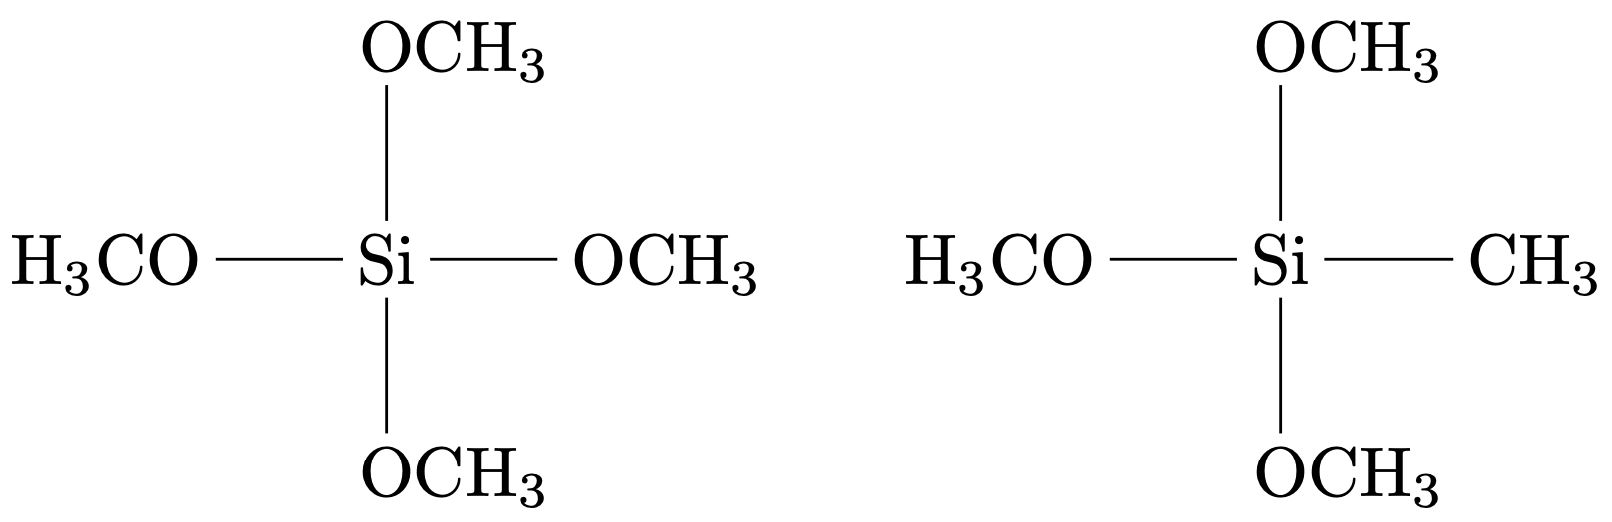
\includegraphics[scale=0.45]{Chapter-4/Figures/precursors.png}
 \caption[Structural formula of the sol-gel precursors used for \textsc{NanoGlass} imprint resist in substrate-conformal imprint lithography (SCIL).]{Structural formula of the sol-gel precursors used for \textsc{NanoGlass} imprint resist: TMOS (\emph{left}; fully inorganic with four methoxy groups) and MTMS (\emph{right}; organically modified with three methoxy groups and one methyl group).}\label{fig:precursors}
 \end{figure}
These precursors, with structural formulas shown in \cref{fig:precursors}, react to form a gel, and ultimately a solid silica-like network, along with alcohols and water left as reaction products \cite{Brinker90,Hench90,Verschuuren10,Verschuuren19}. 
Briefly, methoxy groups (\ce{-O-CH3}) bonded to silicon in TMOS and MTMS undergo hydrolysis so that they are replaced with hydroxyl groups (\ce{-OH}): 
\begin{equation}
 \ce{Si-(O-CH3)} + \ce{H2O} \longrightarrow \ce{Si-OH} + \ce{HO-CH3} , 
 \end{equation}
where methanol (\ce{HO-CH3}) is produced as a reaction product. 
Hydroxylated silicon sites can then react with one another to form a siloxane bond with the release of water: 
\begin{equation}
 \ce{Si-OH} + \ce{HO-Si} \longrightarrow \ce{Si-O-Si} + \ce{H2O} 
 \end{equation}
and as these condensation reactions continue, a silica-like material network is formed. 
This sol-gel process carries out over the course of \SI{15}{\minute} at room temperature while reaction products and trapped air diffuse into the stamp, leaving solidified resist molded to the inverse of the stamp topography after stamp separation. 

The imprinted resist initially has $\sim \SI{70}{\percent}$ the density of fused silica due to the presence of nanoscale pores that result from the organic component of the MTMS precursor (\emph{i.e.}, \ce{Si-CH3} [\emph{cf.\@} \cref{fig:precursors}]), which does not participate in the sol-gel reaction \cite{Verschuuren10,Verschuuren17,Verschuuren19}. 
However, the material can be densified for stability through a \SI{15}{\minute} bake at $T_{\text{cure}} \gtrapprox \SI{50}{\celsius}$ to induce further cross-linking in the material network, where $T_{\text{cure}} \gtrapprox \SI{450}{\celsius}$ breaks the organic bonds in MTMS and causes a moderate level of shrinkage while $T_{\text{cure}} \gtrapprox \SI{850}{\celsius}$ gives rise to the density of maximally cross-linked \ce{SiO2}. 
It has been previously reported that $T_{\text{cure}} \approx \SI{200}{\celsius}$ leads to $\sim \SI{15}{\percent}$ volumetric shrinkage in imprinted laminar gratings while $T_{\text{cure}}$ in excess of $\SI{1000}{\celsius}$ results in a maximal, $\sim \SI{30}{\percent}$ shrinkage \cite{Verschuuren10,Verschuuren19}.   
Based on these results, it is hypothesized that a low-$T_{\text{cure}}$ treatment should lead to $\sim \SI{10}{\percent}$ volumetric shrinkage in the resist, which is comparable to typical levels of imprint-resist shrinkage in UV-NIL \cite{Schift10}. 
To examine the impact on blaze angle in an x-ray reflection grating from this phenomenon, several test replicas of a master grating were produced by \textsc{Philips} and cured at $T_{\text{cure}} \approx \SI{90}{\celsius}$ in an effort to induce a $\sim \SI{10}{\percent}$ shrinkage in the silica sol-gel network. 

\subsection{Master Grating}\label{sec:master_for_SCIL}
%%%%%%%%%%%%%%%%%%%%%%%%%%%%%%%%%%%%%%%%%--------------------------------------------------
The master grating chosen for this study was originally used as a direct stamp for grating fabrication by UV-NIL \cite[\emph{cf.\@} \cref{fig:master_grating,fig:uv_nil}]{Miles18}. 
As summarized in \cref{fig:master_fab}, this \SI{75}{\mm} by \SI{96}{\mm} (\SI{72}{\cm\squared}) grating was fabricated through a multi-step process centering on crystallographic etching in a $\langle 311 \rangle$-oriented, \SI{500}{\um}-thick, \SI{150}{\mm}-diameter silicon wafer. 
The groove layout was a variable-line-space profile defined by EBL with groove spacing, $d$, ranging nominally from \SIrange{160}{158.25}{\nm} along the groove direction, which is aligned with the $\langle 110 \rangle$ direction in the $\{ 311 \}$ plane of the wafer surface [\emph{cf.\@} \cref{sec:crystal_etching}]. 
This layout was then transferred by reactive ion etch into a thin film of low-stress \ce{Si_{x}N_{y}} before the native \ce{SiO2} on the exposed wafer surface was removed with a buffered oxide etch. 
Next, a timed, room-temperature \ce{KOH} etch was carried out to generate the asymmetric sawtooth defined by exposed $\{ 111 \}$ planes that form sharp points at the bottom of each groove with an angle $\theta \equiv \arccos \left( 1/3 \right) \approx 70.5^{\circ}$ [\emph{cf.\@} \cref{eq:Si_angle}]. 
Due to the $\langle 311 \rangle$ surface orientation of the silicon wafer, the exposed $\{ 111 \}$ planes define nominal facet angles of $\delta = 29.5^{\circ}$ and $\bar{\delta} = 180^{\circ} - \theta - \delta \approx 80^{\circ}$ [\emph{cf.\@} \cref{tab:off_axis_si}]. 
A cross-section image of the grating, with the \ce{Si_{x}N_{y}} mask removed by an \ce{HF} soak, is shown under \emph{field-emission scanning electron microscopy (FESEM)} in \cref{fig:master_grating_SEM}. 

Illustrated in \cref{fig:master_grating_profile}, the groove topography resulting from the process just described resembles a series of acute trapezoids with flat tops of width $w$ that each protrude a distance $\Delta h$ of a few \si{\nm} so that the groove depth, $h$, is given approximately by \cref{eq:groove_depth}. 
Although the depth of these sharp grating grooves could not be verified by \emph{atomic force microscopy (AFM)}\footnote{As in \cref{ch:master_fab}, all AFM for this chapter was carried out using a \textsc{Bruker Icon} instrument equipped with a \textsc{SCANASYST-AIR} tip and \textsc{PeakForce Tapping}$^{\text{TM}}$ mode at the Penn State MCL \cite{PSU_MRI_CL,Xu18}.} due to the aspect ratio of the scanning probe tip used for imaging, it is estimated that this quantity falls in the range $\SI{65}{\nm} \lessapprox h \lessapprox \SI{70}{\nm}$ with $w \gtrapprox \SI{30}{\nm}$. 
\begin{figure}
 \centering
 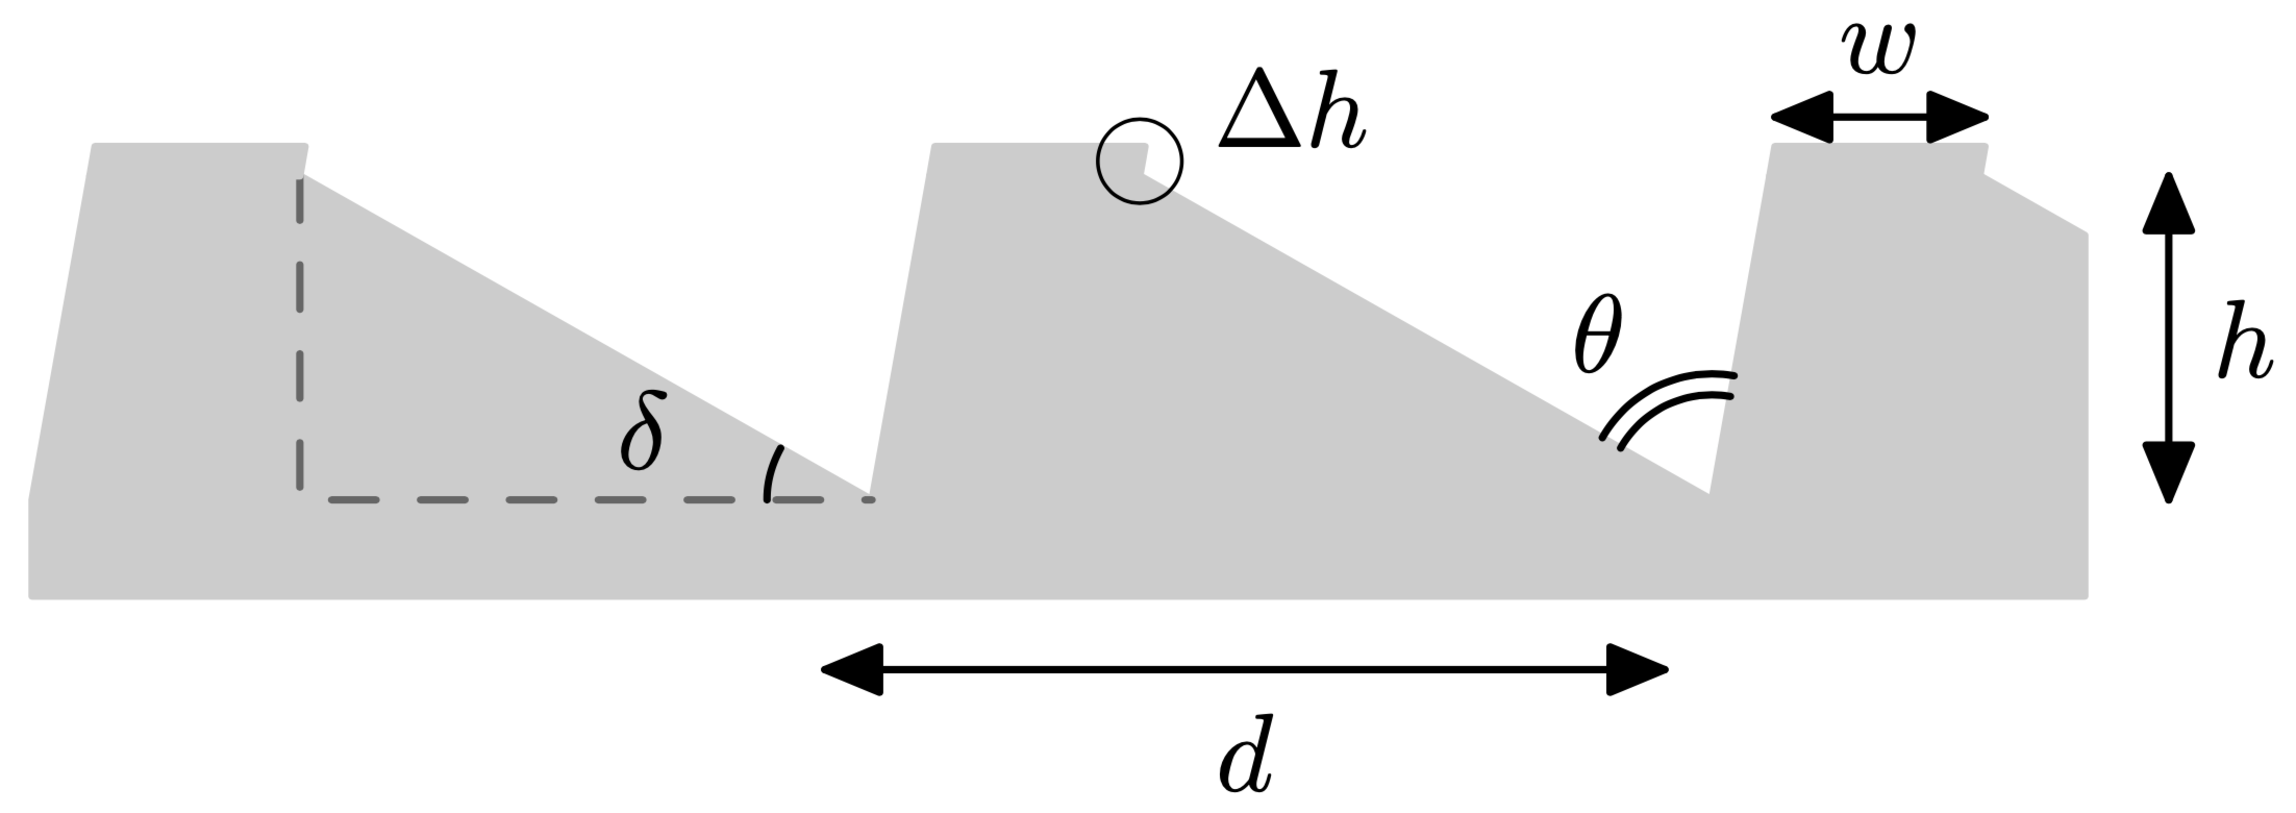
\includegraphics[scale=0.25]{Chapter-4/Figures/master_grating_fab_final.pdf}
 \caption[Illustration of the \ce{KOH}-etched silicon master surface profile]{Illustration of the \ce{KOH}-etched silicon master surface profile from \cref{fig:master_fab} with $\delta = 29.5^{\circ}$ as the nominal blaze angle and $\theta \approx 70.5^{\circ}$ defined by the intersection of exposed $\{ 111 \}$ planes. At a groove spacing of $d \lessapprox \SI{160}{\nm}$, the flat-top regions have widths $w \gtrapprox \SI{30}{\nm}$ as a result of the etch undercut while the groove depth is $\SI{65}{\nm} \lessapprox h \lessapprox \SI{70}{\nm}$ by \cref{eq:groove_depth}. Indicated by the circle, the indented portion of the etched topography cannot be described with a functional form for the diffraction-efficiency analysis in \cref{sec:discussion_scil} \cite{McCoy20b}.}\label{fig:master_grating_profile} 
 \end{figure}
Under AFM, facet surface roughness, $\sigma$ [\emph{cf.\@} \cref{sec:rough_surface}], measures $\lessapprox \SI{0.4}{\nm}$ RMS while the average of \num{30} blaze angle measurements over a \SI{0.5}{\um} by \SI{1}{\um} area yields $\delta = 30.0 \pm 0.8^{\circ}$, where the uncertainty is one standard deviation. 
Although these AFM data were gathered with vertical measurements calibrated to a \SI{180}{\nm} standard, this measurement for $\delta$ is limited in its accuracy due to a relatively poor lateral resolution on the order of a few \si{\nm}. %, at the Penn State Materials Characterization Laboratory,
The measurement is, however, consistent with the nominal value of $\delta = 29.5^\circ$ and is considered a reasonable estimation for the blaze angle of the silicon master, which is constrained through diffraction-efficiency testing in \cref{sec:discussion_scil}. 

\subsection{Stamp Construction}\label{sec:stamp_construction}
%%%%%%%%%%%%%%%%%%%%%%%%%%%%%%%%%%%%%%%%%--------------------------------------------------
Prior to construction of the composite stamp used for imprint production, the silicon master described in \cref{sec:master_for_SCIL} was cleaned in a heated bath of \textsc{Nano-Strip}$^{\text{TM}}$ (\textsc{VWR Int.}), which consists primarily of \emph{sulfuric acid} (\ce{H2SO4}), and then by an oxygen plasma treatment; a top-down FESEM of the cleaned grating is shown in \cref{fig:post_nanostrip}. 
\begin{figure}
 \centering
 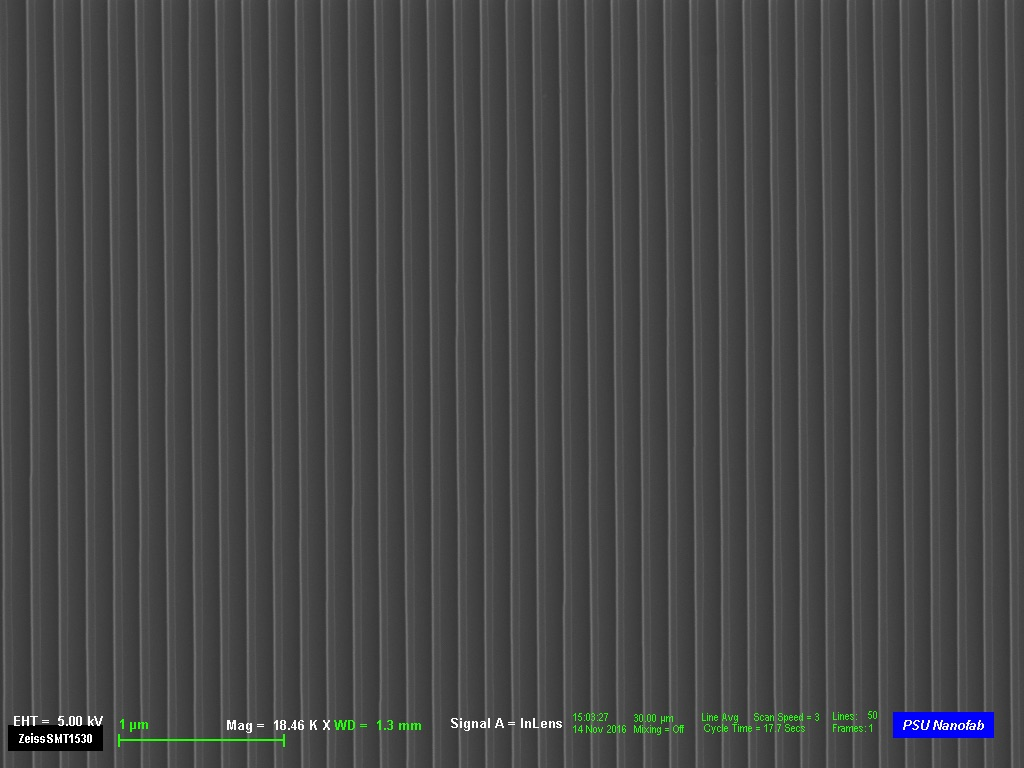
\includegraphics[scale=0.38]{Chapter-4/Figures/post_nanostrip_05.jpg}
 \caption[Top-down FESEM of the silicon master following wafer cleaning.]{Field-emission scanning electron micrograph (FESEM) of the silicon master viewed top-down, following wafer cleaning. Image was taken with a \textsc{Zeiss Leo 1530} instrument at the Penn State Nanofabrication Laboratory as in \cref{fig:master_grating_SEM}.}\label{fig:post_nanostrip}
 \end{figure}
The grating was then surface-treated for anti-stiction with a self-assembled monolayer of perfluorodecyltrichlorosilane (FDTS; \ce{C10H4Cl3F17Si}) \cite{Zhuang07}, which was achieved through a $\SI{50}{\celsius}$ molecular vapor deposition process similar to what is outlined in \cref{sec:nanoimprint}.\footnote{While this wafer cleaning was carried out at Penn State, the surface treatment was performed by \textsc{Philips}. Similar processes using FOTS (\ce{C8H4Cl3F13Si}) [\emph{cf.\@} \cref{fig:FOTS}] were performed by staff at the Cornell NanoScale Science and Technology Facility \cite{Cornell_nano} for SCIL process development carried out at the Quattrone Nanofabrication Facility \cite{Quattrone}.} 
As described by Verschuuren, et~al.~\cite{Verschuuren17} and illustrated in \cref{fig:scil_stamps}(a), a standard SCIL stamp consists of a $\SI{50}{\um}$-thick layer of modified PDMS that carries the inverse topography of the master template, and an underlaying, $\gtrapprox \SI{0.5}{\mm}$-thick layer of standard PDMS that attaches to a flexible, $\SI{200}{\um}$-thick glass sheet by application of an adhesion promoter. 
\begin{figure}
 \centering
 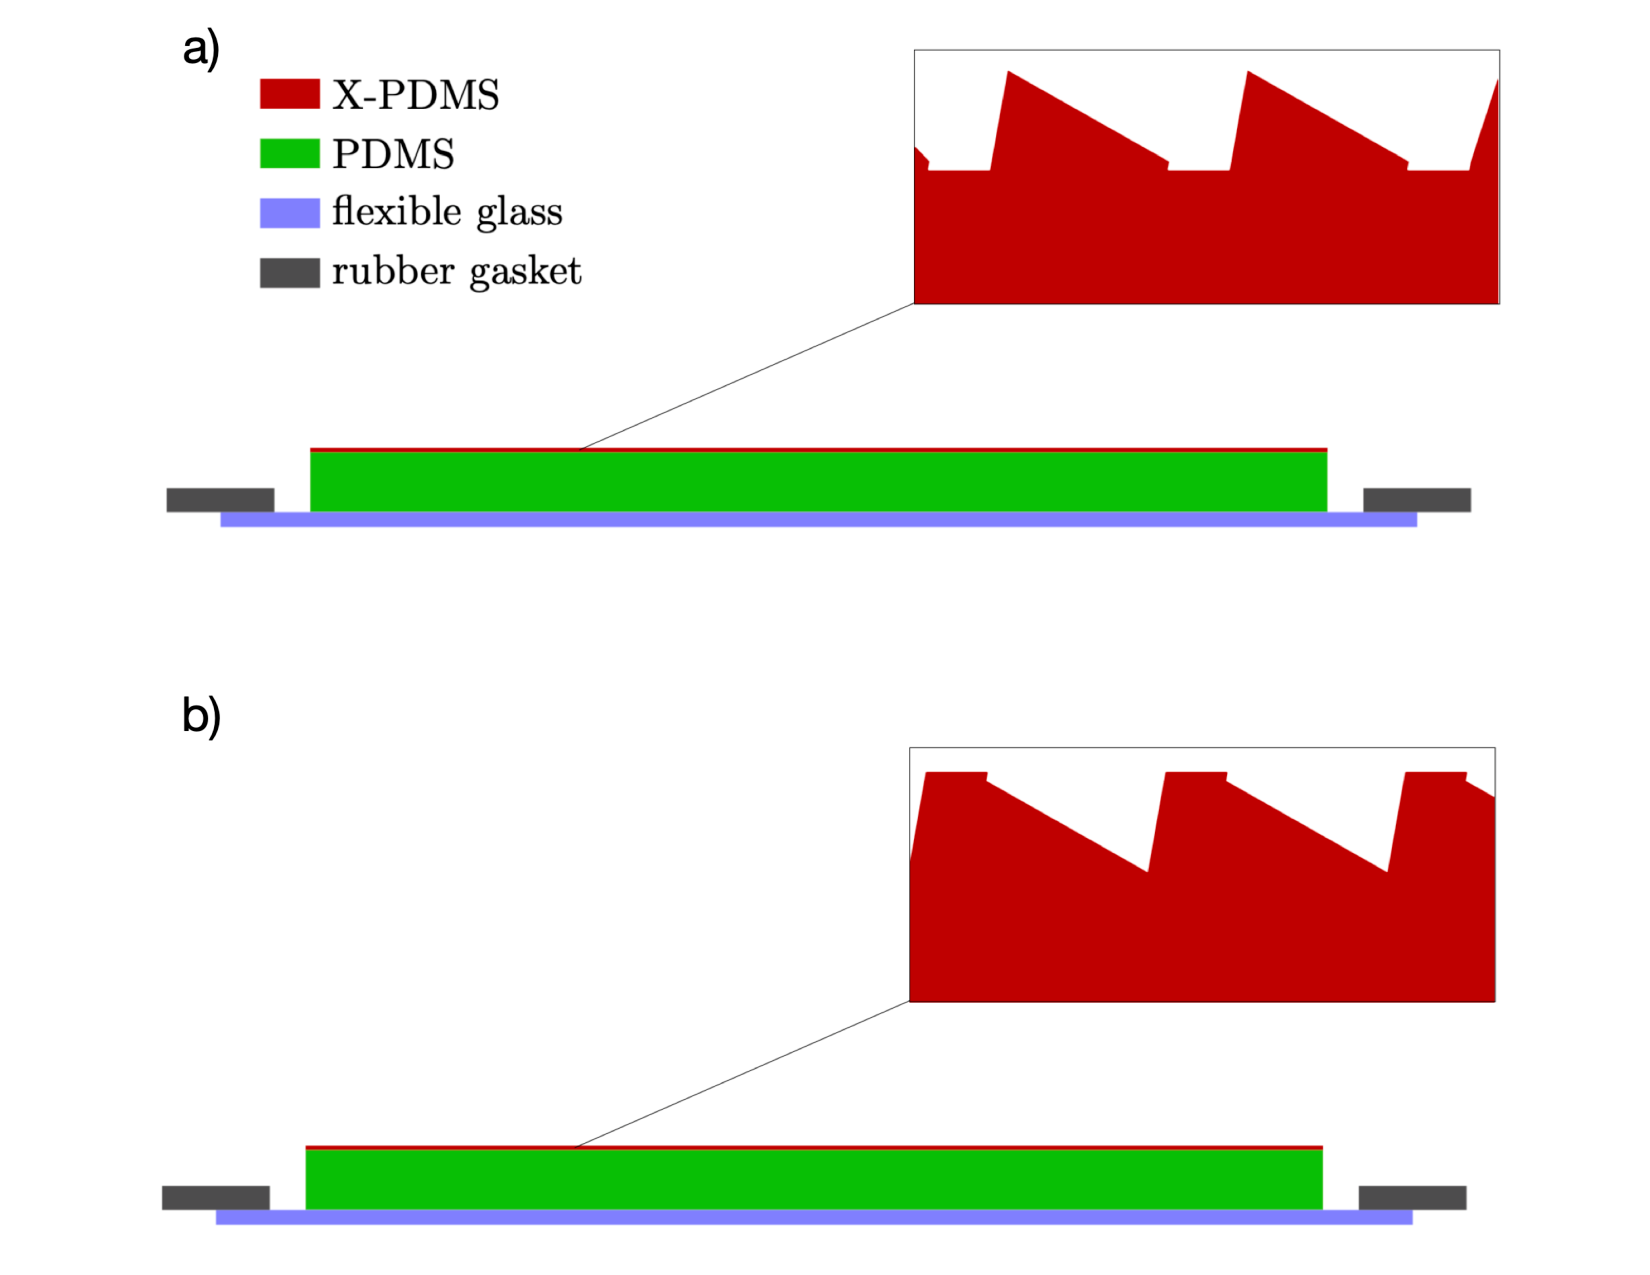
\includegraphics[scale=0.5]{Chapter-4/Figures/SCIL_stamp.pdf}
 \caption[Schematic for SCIL composite stamps of two varieties]{Schematic for SCIL composite stamps of two varieties: a) an initial stamp featuring an inverted topography molded directly from the silicon master and b) a second stamp  featuring a topography similar to the master grating, which was molded using the first stamp as a master template. In either case, grating grooves are carried in a layer of X-PDMS tens of \si{\um} thick that sits on a \SI{200}{\mm}-diameter, flexible glass sheet buffered by a $\gtrapprox \SI{0.5}{\mm}$-thick layer of soft PDMS. A rubber gasket can be attached for use with the pneumatic-based SCIL wafer-scale imprint method. This illustration neglects slight rounding that can occur in sharp corners under the influence of surface tension in X-PDMS \cite{McCoy20b}.}\label{fig:scil_stamps}
 \end{figure}
A rubber gasket can then be glued to the outer perimeter of the square glass sheet for use with the pneumatic-based SCIL wafer-scale imprint method\footnote{This technique is possible with \textsc{AutoSCIL} (for high volume production) or with equipment provided by \textsc{S{\"U}SS MicroTec} that interfaces with a masker aligner (for low-volume production) \cite{philis_scil,suss_microtec}.} to produce imprints with topographies that resemble the silicon master. % shown in \cref{fig:master_grating_profile}.
However, in an effort to produce imprints that emulate the UV-NIL replica described by Miles, et~al.~\cite{Miles18}, which was fabricated using the silicon master as a direct stamp [\emph{cf.\@} \cref{fig:uv_nil_AFM}], this process was modified to construct a stamp with an inverted topography [\emph{cf.\@} \cref{fig:scil_stamps}(b)] so as to allow the production of imprints with sharp apexes and flat portions at the bottom of each groove \cite{Verschuuren18}. 

The variety of modified PDMS used for this study was X-PDMS (v.\ 3), a proprietary material available from \textsc{Philips} \cite{philis_scil}, which was dispensed over the surface of the surface-treated silicon master and then solidified through two rounds of spin-coating and baking steps using primary and accompanying components of the material (\emph{i.e.}, the X-PDMS that carries the groove shape and an additional \emph{intermediate layer}) \cite{Verschuuren17}. 
First, after the silicon master was cleaned again using deionized water (\ce{H2O}) and isopropyl alcohol (\ce{C3H8O}), $\sim \SI{3}{\gram}$ of the primary component was dispensed through a short spin-coat process at \num{2000} rotations per \si{\minute} using a low spin acceleration, leaving a layer tens of \si{\um} thick. 
This was followed immediately by a $\SI{50}{\celsius}$ hotplate bake for \SI{3}{\minute} and a room-temperature cool-down of \SI{10}{\minute}, leaving the material in a tacky state. 
Next, $\sim \SI{3}{\gram}$ of the accompanying component was spin-coated over this material in a similar way before the wafer was baked by hotplate at \SI{70}{\celsius} for \SI{10}{\minute} to form an intermediate layer also tens of \si{\um} thick. 
The doubly-coated silicon master was then oven-baked at $\SI{75}{\celsius}$ for \SI{20}{\hour}, forming a $\sim \SI{50}{\um}$-thick layer of cured X-PDMS with a Young's modulus on the order of several tens of \si{\mega\pascal}. 
In principle, this level of stiffness is sufficient for the stamp to carry $d \lessapprox \SI{160}{\nm}$ grating grooves without pattern distortion or feature collapse \cite{Verschuuren17,Verschuuren19}. 
\begin{figure}
 \centering
 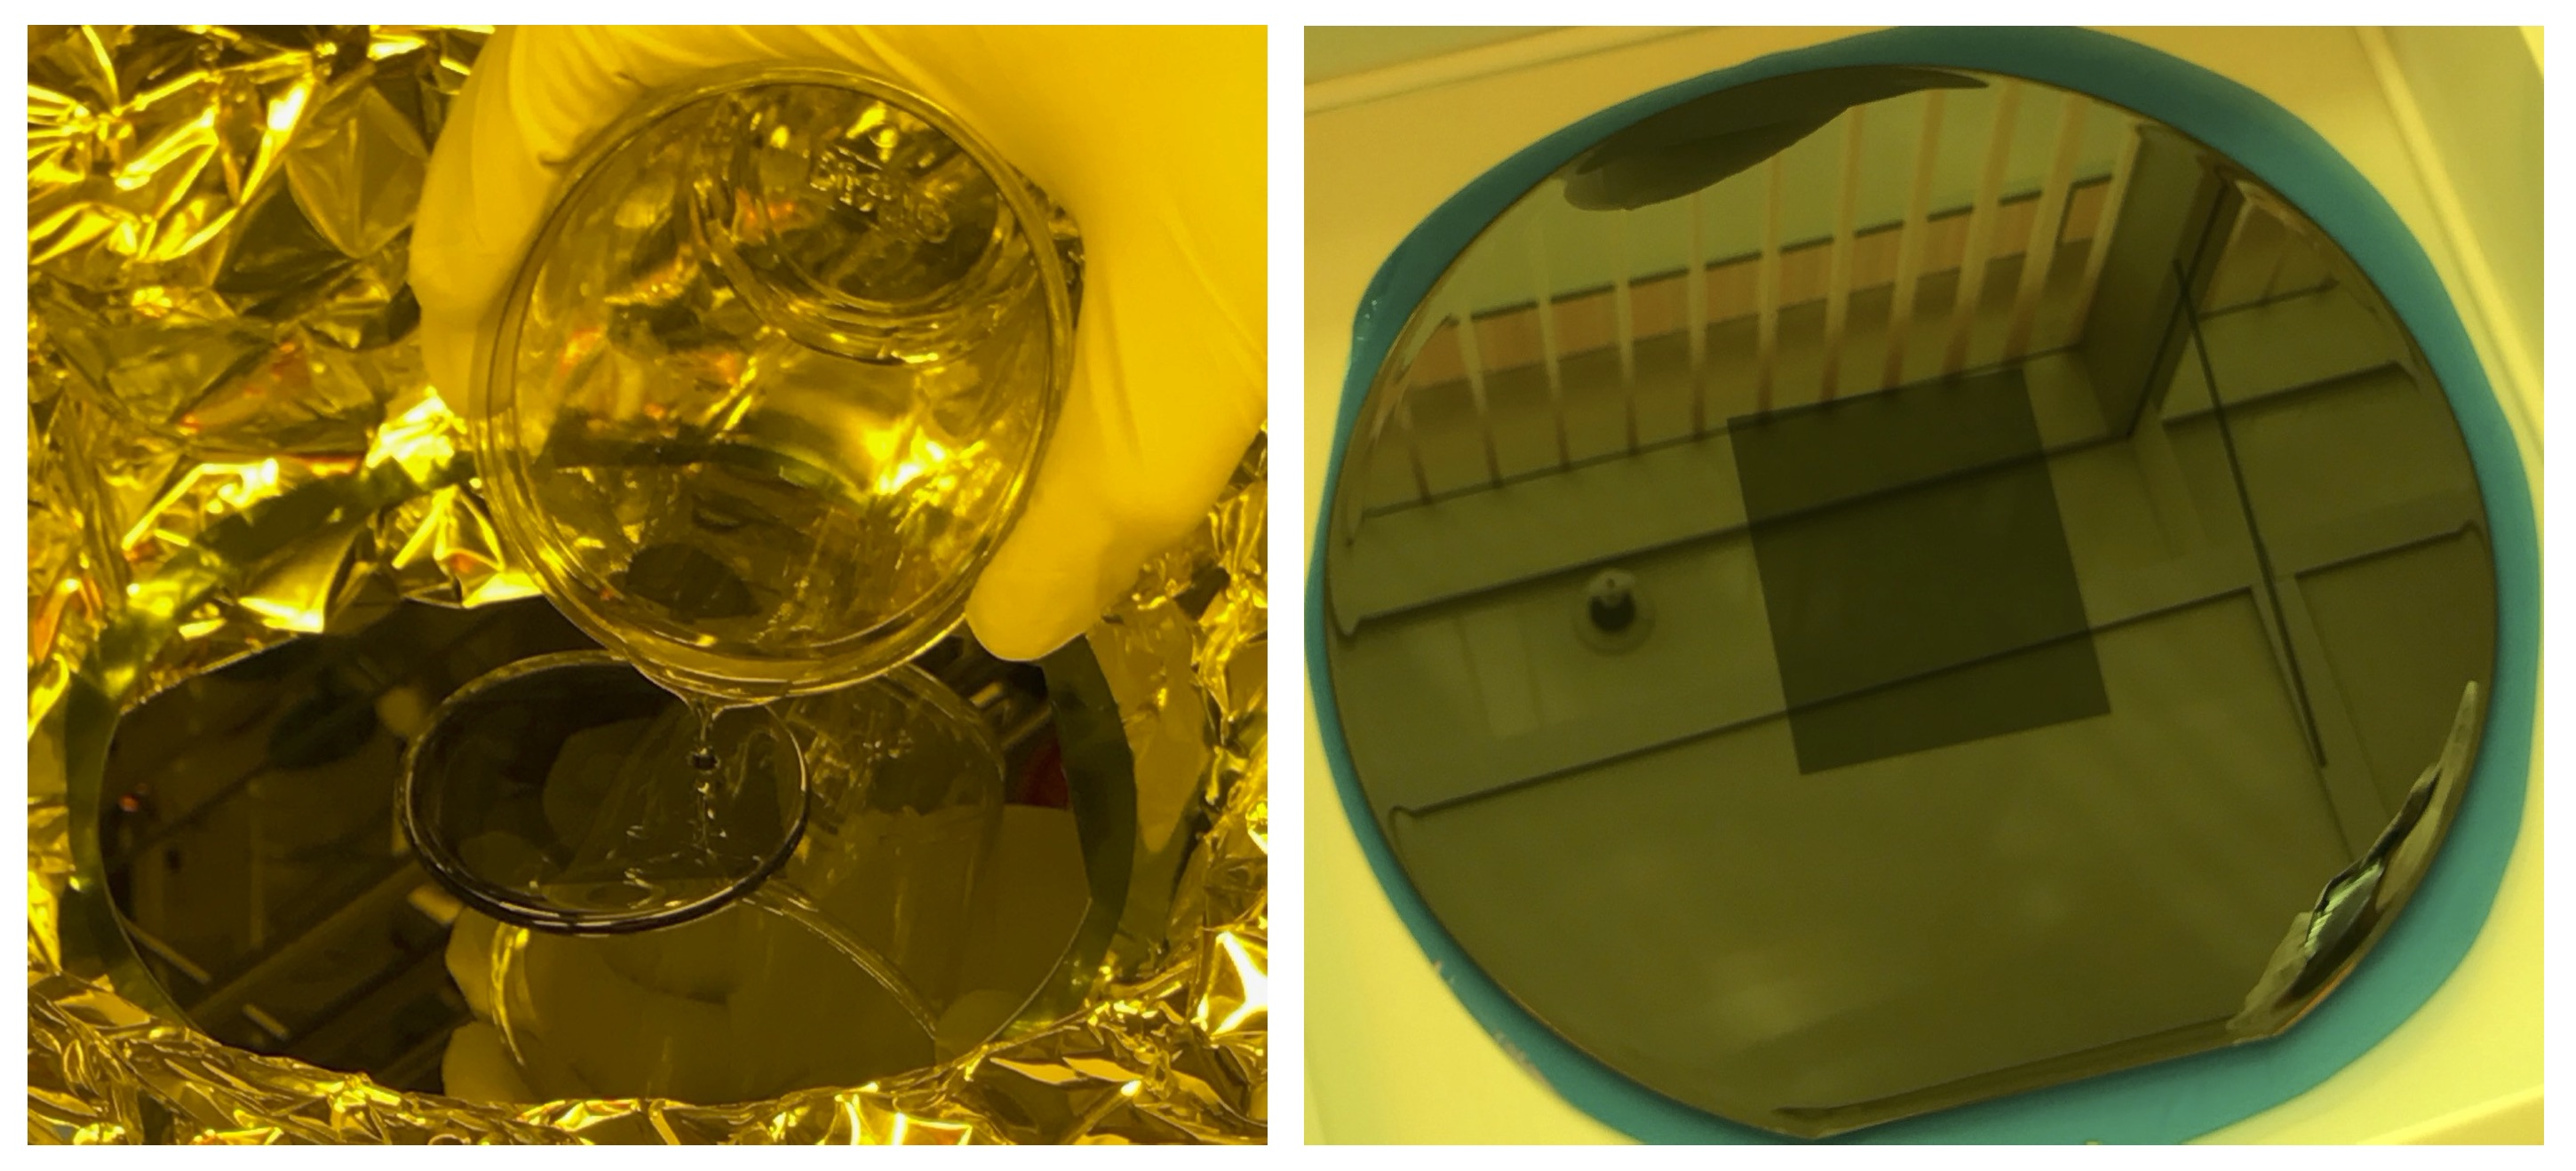
\includegraphics[scale=0.15]{Chapter-4/Figures/SCIL_UPenn_spin.jpg}
 \caption[A \SI{150}{\mm}-diameter, \ce{KOH}-etched, $\langle 100 \rangle$ silicon grating spin-coated with H-PDMS at the Quattrone Nanofabrication Facility (QNF).]{A \SI{150}{\mm}-diameter silicon master spin-coated with H-PDMS at Quattrone Nanofabrication Facility (QNF). Due to the high viscosity of the material, a gradual spin acceleration must be used to achieve a uniform layer \cite{McCoy17}.}\label{fig:UPenn_spin}
 \end{figure}
A similar silicon master\footnote{The grating shown in \cref{fig:UPenn1} was fabricated by staff at the Penn State Nanofabrication Laboratory \cite{PSU_MRI_nanofab} in a similar fashion to the master grating described in \cref{sec:master_for_SCIL}: parallel lines and spaces with $d = \SI{160}{\nm}$ were patterned over a \SI{40}{\mm} by \SI{50}{\mm} (\SI{20}{\cm\squared}) area by EBL before the pattern was transferred into $\langle 100 \rangle$-oriented silicon through a \ce{KOH} etch to yield a symmetric, sawtooth-like topography with an effective blaze angle of $\delta = 54.74^{\circ}$ [\emph{cf.\@} \cref{fig:KOH_geo,tab:off_axis_si}].} coated with H-PDMS at the Quattrone Nanofabrication Facility (QNF) \cite{Quattrone} is shown in \cref{fig:UPenn_spin}. 

Using the SCIL \emph{Stamp Making Tool (SMT)} built by \textsc{Philips}, the initial, non-inverted stamp was formed by curing soft, \textsc{Sylgard 184} PDMS (\textsc{Dow, Inc.}) between the X-PDMS layer and a \SI{200}{\um}-thick sheet of \textsc{D 263} glass (\textsc{Schott AG}) cut into a circle with a \SI{200}{\mm} diameter. 
Consisting primarily of two opposite-facing vacuum chucks heated to $\SI{50}{\celsius}$ with surfaces flat to $\lessapprox \SI{10}{\um}$ peak-to-valley, this tool was used to spread $\sim \SI{12}{\gram}$ of degassed PDMS evenly over the X-PDMS layer. 
With the doubly-coated master secured to the bottom chuck, the \textsc{D 263} glass sheet secured to the top chuck was carefully brought into contact with the PDMS and then slowly clamped down using micrometer spindles to form a uniformly-thick layer while ensuring that the two chuck surfaces are parallel to within \SI{20}{\um}. 
These materials were baked in this configuration at \SI{50}{\celsius} until the PDMS was cured before the stamp was carefully separated from the silicon master. 
Using the initial, non-inverted stamp as a master template, the second, inverted stamp was then constructed on a square sheet of glass through steps identical to those outlined above. 
This processing was enabled by the first stamp being constructed on a round sheet of glass, which allowed it to be spin-coated with X-PDMS and subsequently cured like the silicon master. 

As an additional item for clarification, laboratory space for a similar SCIL stamp-making process carried out at QNF is pictured in the top panel of \cref{fig:UPenn1}. 
\begin{figure}
 \centering
 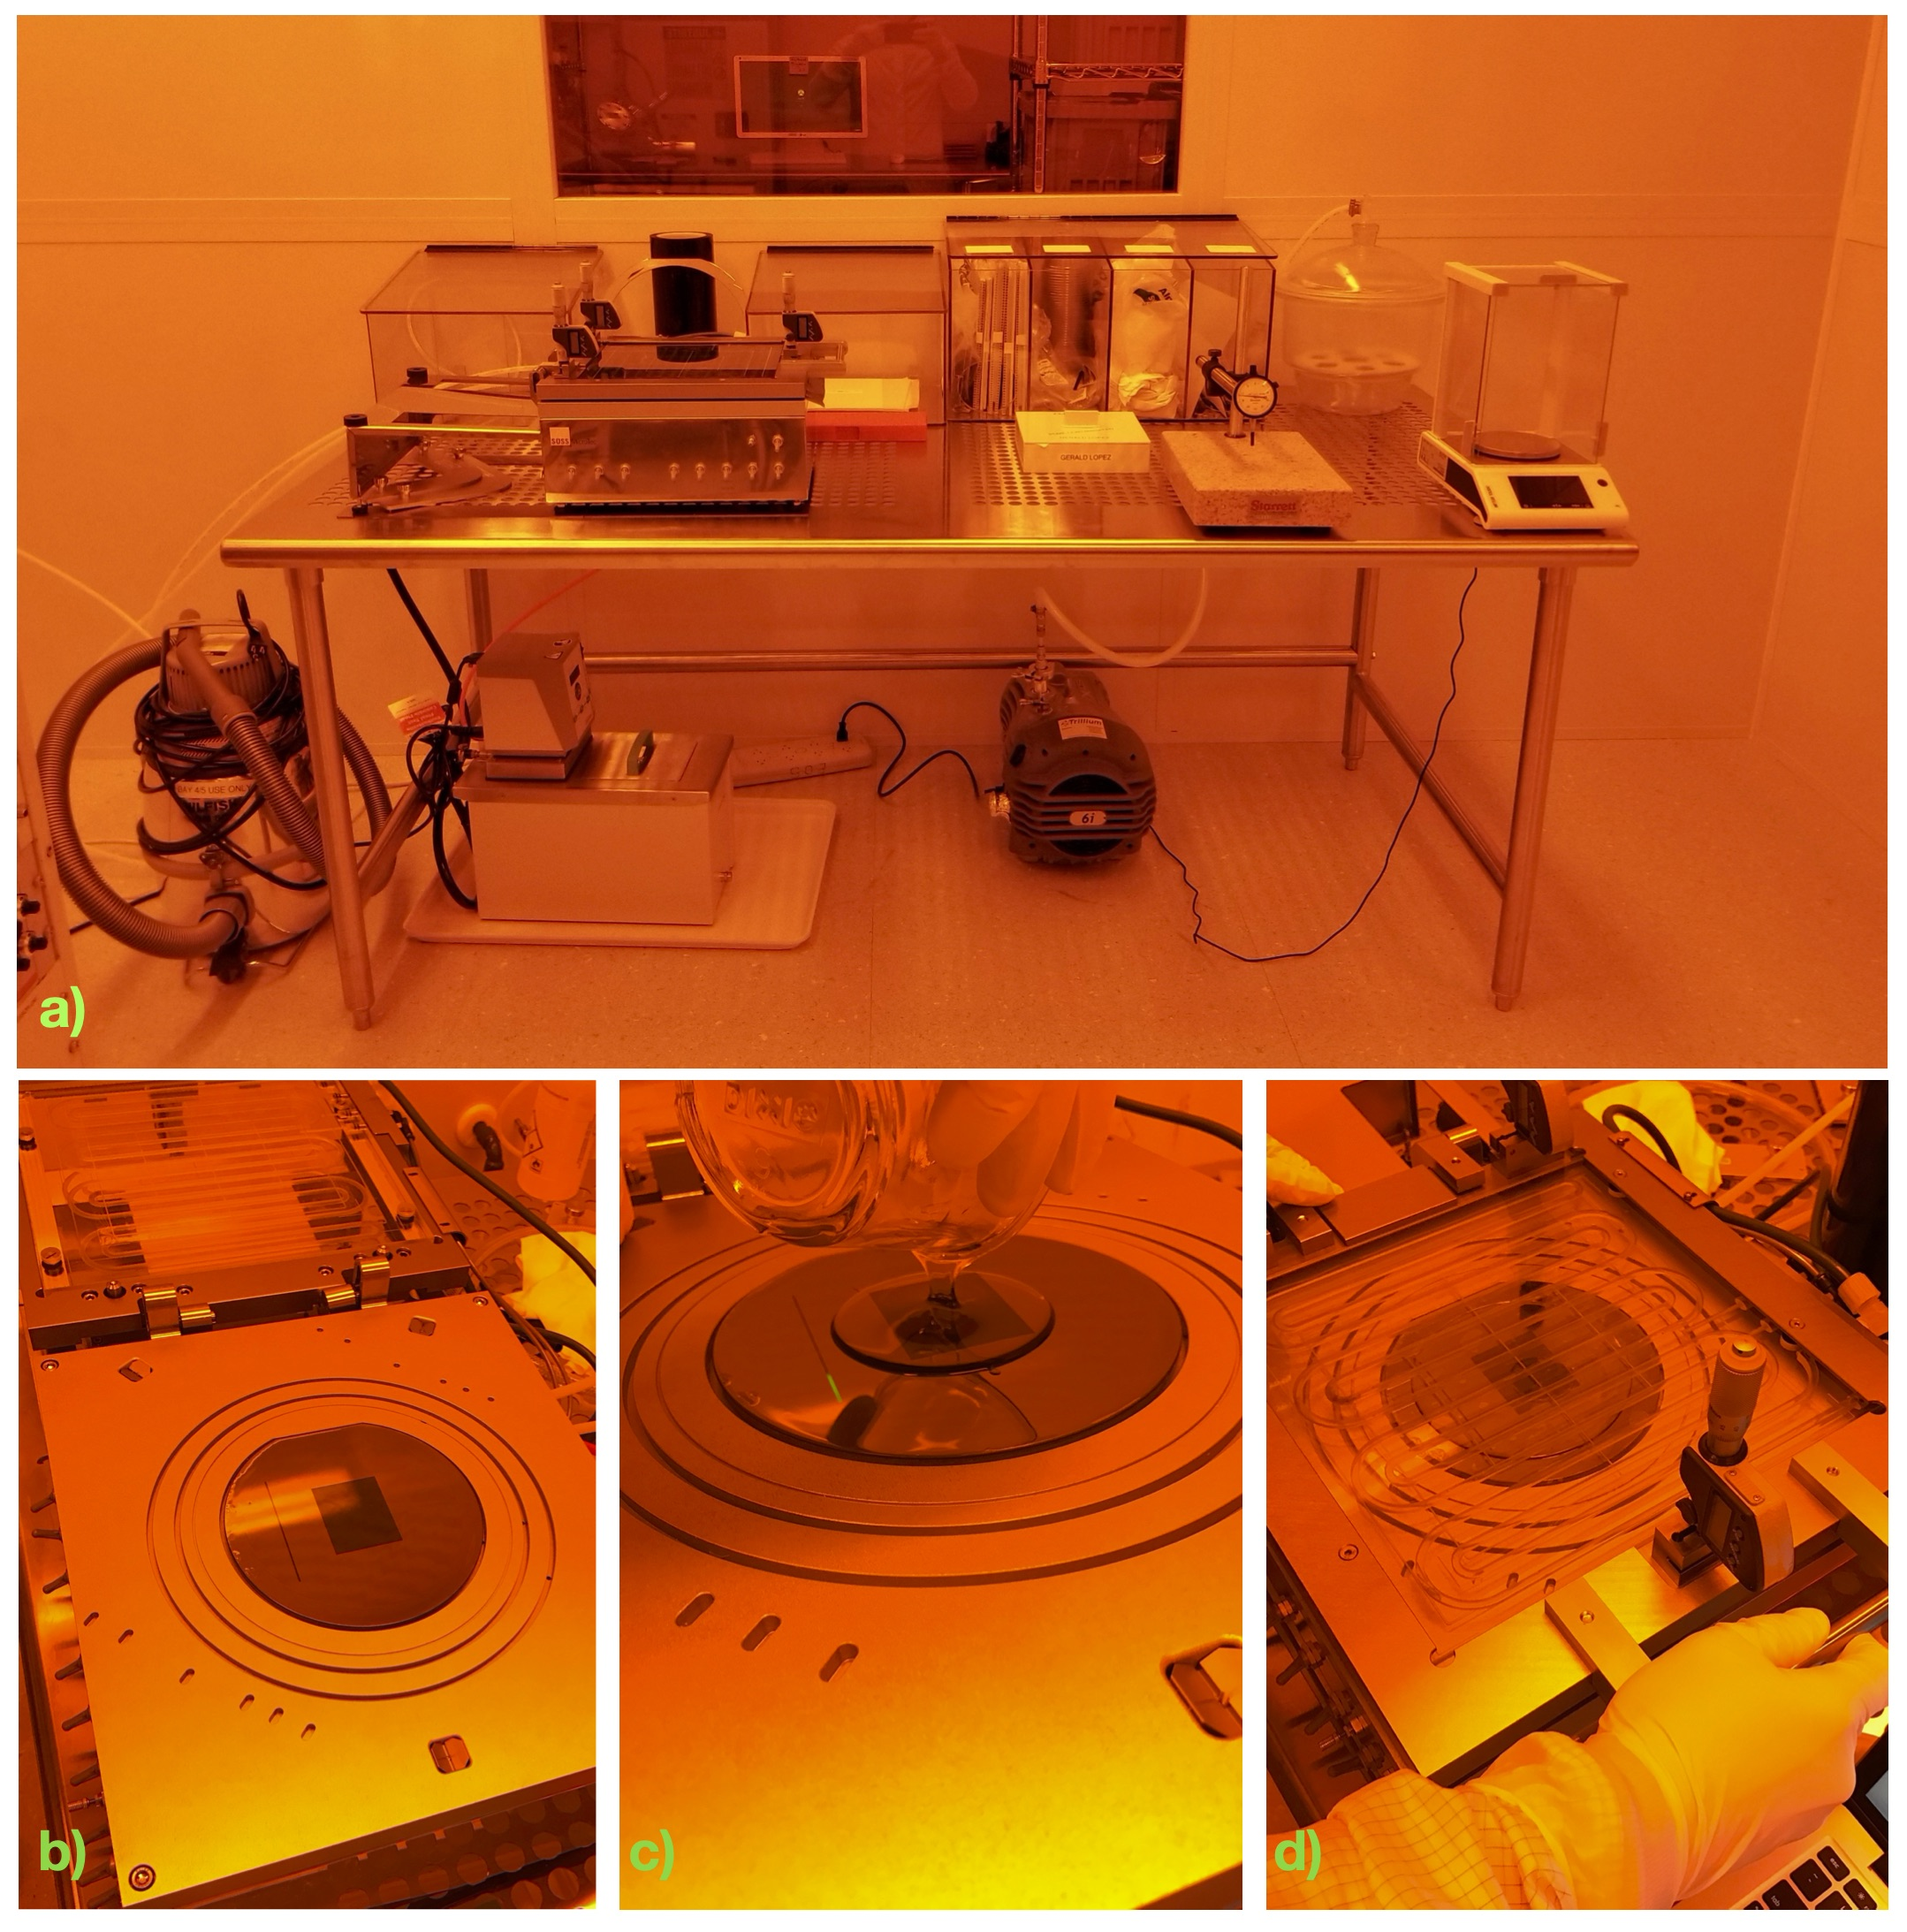
\includegraphics[scale=0.19]{Chapter-4/Figures/SCIL_UPenn1.jpg}
 \caption[SCIL stamp construction at QNF]{SCIL stamp construction at QNF: a) laboratory space featuring an MRT (\textsc{S{\"U}SS MicroTec} \cite{suss_microtec}) and supporting equipment for surface heating and PDMS preparation, b) heated surfaces on the MRT for the silicon master and a flexible sheet of glass on the inside of the MRT lid, c) PDMS is poured over the surface of the silicon master, d) the MRT lid is closed and the PDMS is cured at \SI{50}{\celsius} \cite{McCoy17}.}\label{fig:UPenn1}
 \end{figure}
Making use of the \emph{Master Replication Tooling (MRT)} built by \textsc{S{\"U}SS MicroTec} \cite{suss_microtec}, which provides the functionality of the SMT, the bottom panels of \cref{fig:UPenn1} show steps involved with curing \textsc{Sylgard 184} PDMS in between the master grating template spin-coated with H-PDMS from \cref{fig:UPenn_spin}. 
First, the coated master is secured on a surface heated to \SI{50}{\celsius} with a vacuum chuck provided by the MRT; a clean sheet of \textsc{AF32} glass (\textsc{Schott AG}) is also secured to a heated vacuum chuck on the inside of the MRT lid.  
\textsc{Sylgard 184} PDMS is then carefully poured over the surface of the master before the top chuck is carefully brought in contact before micrometer spindles are used to spread the material evenly over the wafer surface. 
After the materials have been cured, the MRT is opened and the SCIL stamp is carefully separated from the silicon master. 

\subsection{Imprint Production}\label{sec:imprint_production}
%%%%%%%%%%%%%%%%%%%%%%%%%%%%%%%%%%%%%%%%%--------------------------------------------------
Performed by \textsc{Philips}, several blazed-grating surface reliefs were imprinted by hand into $\sim \SI{100}{\nm}$-thick films of \textsc{NanoGlass T1100} sol-gel resist spin-coated on \SI{1}{\mm}-thick, \SI{150}{\mm}-diameter silicon wafers using the inverted X-PDMS stamp described in \cref{sec:stamp_construction}.  
\begin{figure}
 \centering
 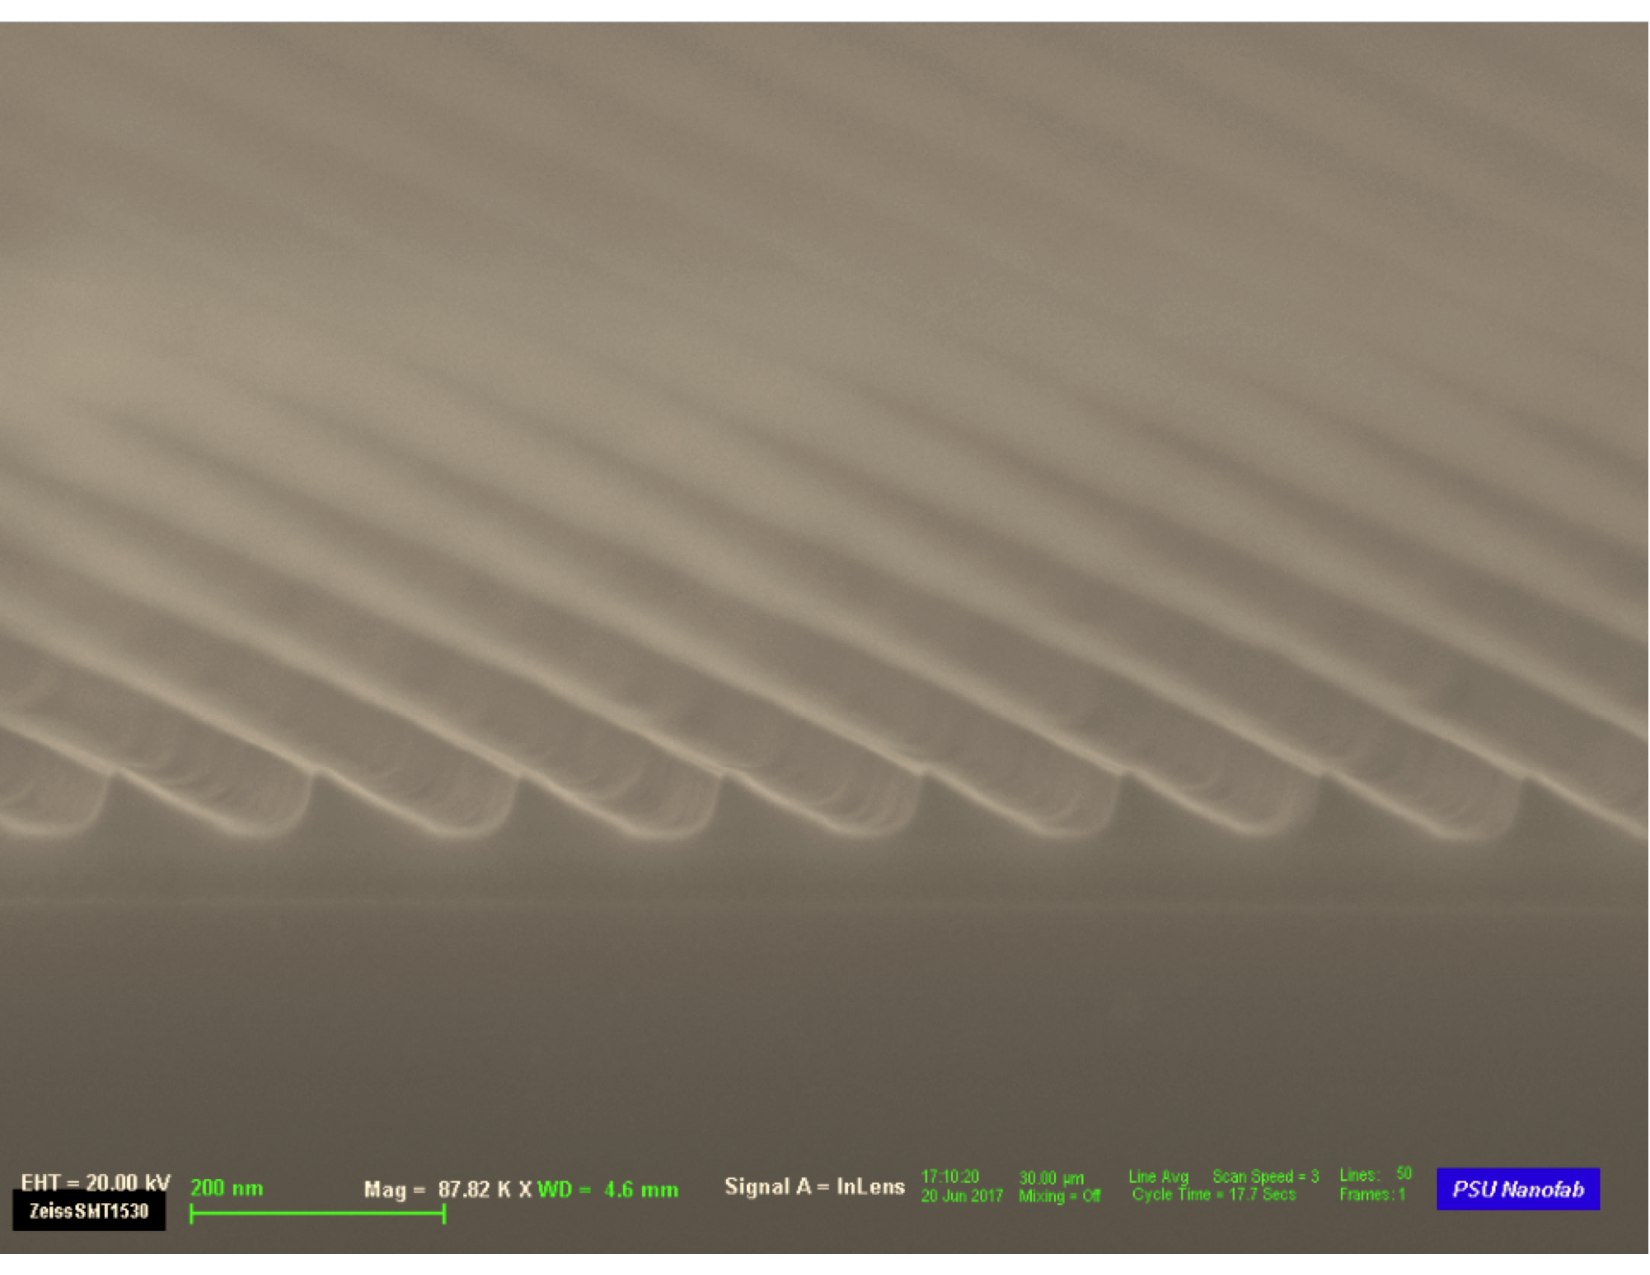
\includegraphics[scale=0.5]{Chapter-4/Figures/scil_replica.pdf}
 \caption[Cross-section FESEM of a grating imprint in \textsc{NanoGlass T1100}]{Cross-section FESEM of a grating imprint with $d \lessapprox \SI{160}{\nm}$ in $\sim \SI{100}{\nm}$-thick \textsc{NanoGlass T1100} sol-gel resist coated on a silicon wafer. This topography was produced from an inverted composite stamp [\emph{cf.\@} \cref{fig:scil_stamps}(b)]. Image was taken with a \textsc{Zeiss Leo 1530} instrument as in \cref{fig:master_grating_SEM,fig:post_nanostrip} \cite{McCoy17,McCoy20b}.}\label{fig:SCIL_SEMs} %and then baked to $\SI{90}{\celsius}$ following stamp separation
\end{figure} 
Although the pneumatic-based SCIL wafer-scale imprint method (\emph{e.g.}, via \textsc{AutoSCIL}) is best equipped for minimizing pattern distortion over \SI{150}{\mm} wafers, imprinting by hand is sufficient for producing a small number of grating molds suitable for the diffraction-efficiency testing described in \cref{sec:beamline_testing}, which depends primarily on groove facet shape over a local area defined by the projected size of the monochromatic beam at the ALS [\emph{cf.\@} \cref{sec:als_beam}]. 
\begin{figure}
 \centering
 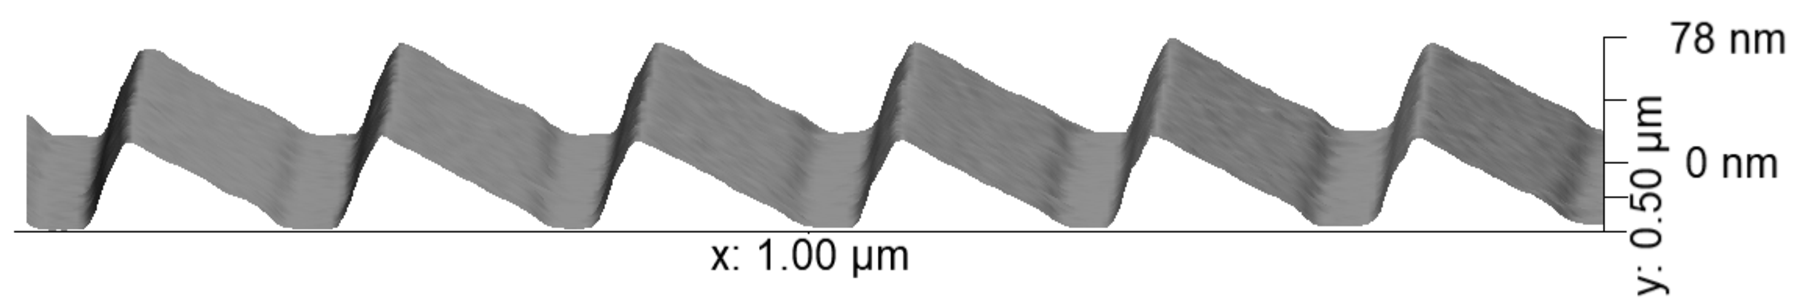
\includegraphics[scale=0.52]{Chapter-4/Figures/AFM_bare.pdf}
 \caption[AFM of a grating imprint in \textsc{NanoGlass T1100}]{AFM of a grating imprint with $d \lessapprox \SI{160}{\nm}$ in $\sim \SI{100}{\nm}$-thick \textsc{NanoGlass T1100} sol-gel resist coated on a silicon wafer as in \cref{fig:SCIL_SEMs}. Facet roughness and blaze angle under AFM measure $\sigma \approx \SI{0.6}{\nm}$ RMS and $27.9 \pm 0.7^{\circ}$, respectively \cite{McCoy17,McCoy20b}.}\label{fig:SCIL_AFMs} 
 \end{figure}
With imprinting taking place at room temperature, \SI{15}{\minute} of stamp-resist contact was required for the sol-gel process to carry out. 
Each wafer following stamp separation was baked by hotplate to $\SI{90}{\celsius}$ for \SI{15}{\minute} to densify the imprinted material to a small degree, thereby inducing resist shrinkage. 
An imprinted replica produced in this way is shown under FESEM in \cref{fig:SCIL_SEMs}, where grating grooves are seen imprinted over a residual layer of resist several tens of \si{\nm} thick. 
An identical imprint is shown under AFM in \cref{fig:SCIL_AFMs}, where the average blaze angle measures $\delta' = 27.9 \pm 0.7^{\circ}$, giving a $\delta' / \delta \approx 0.93$ or $\delta - \delta' \approx 2^{\circ}$ reduction in blaze angle relative to $\delta = 30.0 \pm 0.8^{\circ}$ measured for the silicon master \cite[\emph{cf.\@} \cref{sec:master_for_SCIL}]{McCoy20b}. 

\section{Beamline Experiments}\label{sec:beamline_testing}
%%%%%%%%%%%%%%%%%%%%%%%%%%%%%%%%%%%%%%%%%-------------------------------------------------- 
This section describes how the reduced blaze angle of the SCIL replica described in \cref{sec:grating_fab} is verified through beamline testing by comparing its diffraction-efficiency response in the soft x-ray to that of the silicon master. 
These experiments for measuring \emph{absolute diffraction efficiency}, $\mathscr{E}_n$, took place at beamline 6.3.2 of the ALS \cite{ALS_632,Underwood96,Gullikson01} using methodology similar to \cref{sec:taste_eff_results} for TASTE prototype testing.  %similar to \cref{sec:taste_eff_results}.
Discussed in \cref{sec:als_testing}, this facility provides a monochromatic beam of EUV radiation and soft x-rays with photon energy, $\mathcal{E}_{\gamma} = h c_0 / \lambda$, up to \SI{1300}{\electronvolt}. 
Radiation with $\mathcal{E}_{\gamma} < \SI{440}{\electronvolt}$, however, requires the use of a triple-mirror order sorter to ensure a spectrally pure beam [\emph{cf.\@} \cref{sec:als_beam}]. 
%Although $\alpha$ and $\gamma$ are controlled 
With a specified grating geometry being established through the movement of stage rotations at the beamline [\emph{cf.\@} \cref{sec:geo_constrain}], the implementation of this order sorter can cause a slight beam shift that serves to perturb a precisely-set grating geometry; because of this, $\mathcal{E}_{\gamma} = \SI{440}{\electronvolt}$ was chosen as the lower limit for diffraction-efficiency testing. 

The silicon master was tested without a reflective overcoat to maintain its sharply defined surface-relief profile whereas the SCIL replica was coated with a thin layer of gold, using chromium as an adhesion layer, in an effort to emulate the UV-NIL replica described by Miles, et~al.~\cite[\emph{cf.\@} \cref{sec:nanoimprint}]{Miles18}. 
\cref{sec:reflectivity} describes how the upper photon-energy limit for testing was determined from considering Fresnel reflectivity for silicon and gold surfaces at a grazing-incidence angle $\zeta \approx 1.7^{\circ}$ [\emph{cf.\@} \cref{eq:angle_on_groove,eq:graze_angle}]: 
\begin{equation}
 \sin \left( \zeta \right) = \sin \left( \eta \right) \frac{\cos \left( \alpha - \delta \right)}{\cos \left( \alpha \right)} \implies \sin \left( \zeta \right) \approx \sin \left( \eta = 1.5^{\circ} \right) \sec \left( \delta = 29.5^{\circ} \right) ,
 \end{equation}
where $\eta = 1.5^{\circ}$ is the graze angle relative to the optic mount surface used by Miles, et~al.~\cite{Miles18} and $\alpha \approx \delta$ is the azimuthal incidence angle in a near-Littrow configuration with $\delta = 29.5^{\circ}$ as the nominal blaze angle of the silicon master described in \cref{sec:grating_fab}.\footnote{These angles are defined geometrically in \cref{fig:conical_reflection_edit,fig:grating_angles}.}
Following this, \cref{sec:grat_geo_scil,sec:test_results_scil}, describe how test geometries were constrained and present the gathered diffraction-efficiency data, respectively.  

\subsection{Reflectivity Considerations}\label{sec:reflectivity}
%%%%%%%%%%%%%%%%%%%%%%%%%%%%%%%%%%%%%%%%%-------------------------------------------------- 
To model the surface the silicon master, a thin layer of native \ce{SiO2} is taken into account so that an expression for specular reflectivity is determined from phase-matching the electromagnetic fields at a boundary between vacuum and \ce{SiO2}, as well as an accompanying boundary between \ce{SiO2} and the silicon substrate. 
Although the monochromatic beam at the ALS is \emph{s-polarized} to a high degree, Fresnel reflectivity in the soft x-ray is virtually polarization-independent at grazing-incidence angles [\emph{cf.\@} \cref{sec:als_beam,sec:reflectivity_polarization}]. 
Taking $\tilde{\nu}_1$ as the complex index of refraction for \ce{SiO2}, the complex reflection coefficient for the first interface in s-polarization, which is approximately equal to the corresponding term in \emph{p-polarization}, is [\emph{cf.\@} \cref{eq:refl_coeff01}]
\begin{subequations}
\begin{equation}
 \tilde{r}_{0,1} = \frac{k_{\perp,0} - \tilde{k}_{\perp,1}}{k_{\perp,0} + \tilde{k}_{\perp,1}} = \frac{\sin \left( \zeta \right) - \sqrt{\tilde{\nu}_1^2 - \cos^2 \left( \zeta \right)}}{\sin \left( \zeta \right) + \sqrt{\tilde{\nu}_1^2 - \cos^2 \left( \zeta \right)}} ,
 \end{equation}
where $k_{\perp,0} = -k_0 \sin \left( \zeta \right)$ and $\tilde{k}_{\perp,1} = -k_0 \sqrt{\tilde{\nu}_1^2 - \cos^2 \left( \zeta \right)}$ are the components of the wave vector normal to the boundary in vacuum and in \ce{SiO2}, respectively, with $k_0 \equiv 2 \pi / \lambda$ as the wave number in vacuum. 
Similarly, with $\tilde{\nu}_2$ as the refractive index for silicon, the reflection coefficient for the second interface in the same polarization is [\emph{cf.\@} \cref{eq:refl_coeff12}] 
\begin{equation}
 \tilde{r}_{1,2} = \frac{\tilde{k}_{\perp,1} - \tilde{k}_{\perp,2}}{\tilde{k}_{\perp,1} + \tilde{k}_{\perp,2}} = \frac{ \sqrt{\tilde{\nu}_1^2 - \cos^2 \left( \zeta \right)} - \sqrt{\tilde{\nu}_2^2 - \cos^2 \left( \zeta \right)} }{ \sqrt{\tilde{\nu}_1^2 - \cos^2 \left( \zeta \right)} + \sqrt{\tilde{\nu}_2^2 - \cos^2 \left( \zeta \right)}} , 
 \end{equation}
\end{subequations}
where $\tilde{k}_{\perp,2} = -k_0 \sqrt{\tilde{\nu}_2^2 - \cos^2 \left( \zeta \right)}$ is the component of the wave vector normal to the surface in silicon. 
Using $\tilde{r}_{0,1}$ and $\tilde{r}_{1,2}$, the overall specular reflectivity for a silicon substrate with a native-oxide layer of thickness $\tau$ can be written as the norm-squared of \cref{eq:refl_coeff_example} for a thin film:
\begin{equation}\label{eq:Si_layer_refl}
 \mathcal{R}_{\text{film}} = \norm{ \frac{\tilde{r}_{0,1} + \tilde{r}_{1,2} \mathrm{e}^{-2i \tilde{k}_{\perp,1} \tau}}{1 + \tilde{r}_{0,1} \tilde{r}_{1,2} \mathrm{e}^{-2i \tilde{k}_{\perp,1} \tau}} }^2 .
 \end{equation}
%with $i \equiv \sqrt{-1}$ as the imaginary unit. 

The absorbing effect of surface roughness in the limit of very small lateral size scales can be taken into account by modulating $\tilde{r}_{0,1}$ and $\tilde{r}_{1,2}$ by the following \emph{Nevot-Croce factors} [\emph{cf.\@} \cref{sec:refl_account}]:
\begin{equation}\label{eq:NC_factors}
 \tilde{r}_{0,1} \to \tilde{r}_{0,1} \mathrm{e}^{-2 k_{\perp,0} \tilde{k}_{\perp,1} \sigma_1^2} \quad \text{and} \quad \tilde{r}_{1,2} \to \tilde{r}_{1,2} \mathrm{e}^{-2 \tilde{k}_{\perp,1} \tilde{k}_{\perp,2} \sigma_2^2} ,
 \end{equation}
where $\sigma_1$ and $\sigma_2$ are the RMS roughness values for the surface of the \ce{SiO2} film and the underlaying boundary between \ce{SiO2} and the silicon substrate, respectively. 
 \begin{figure}
 \centering
 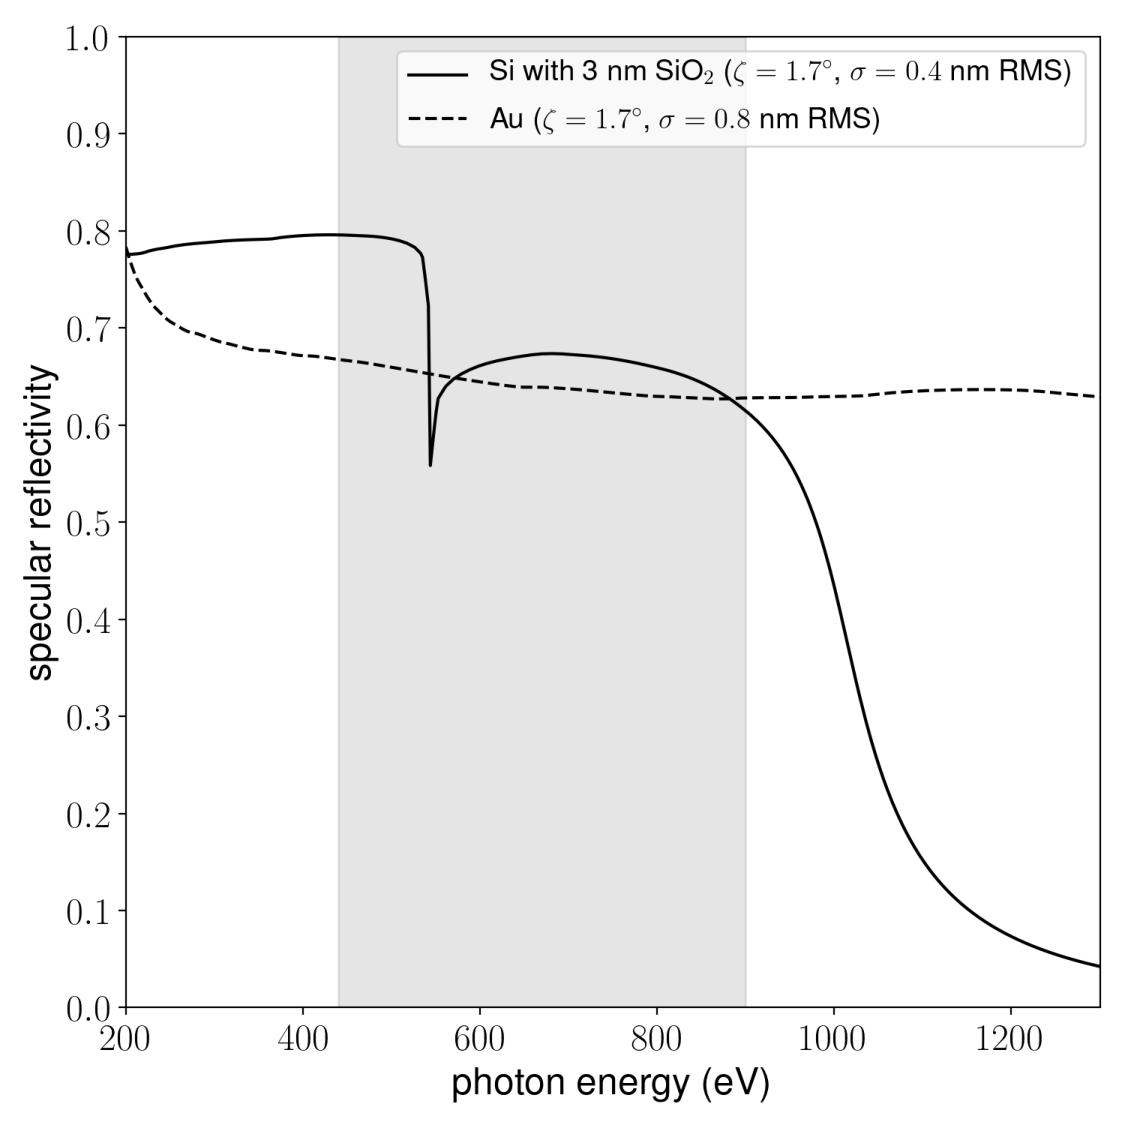
\includegraphics[scale=0.6]{Chapter-4/Figures/reflectivity_plot.pdf}
 \caption[Specular reflectivity curves for a silicon substrate and a thick slab of gold at a $1.7^{\circ}$ graze angle]{Specular reflectivity curves for a silicon substrate with \SI{3}{\nm} of native oxide (solid line) and a thick slab of gold (dashed line) for a $1.7^{\circ}$ graze angle, which are indicative of the overall responses expected for the silicon master and the coated SCIL replica, respectively. Because the use of the order sorter at the beamline (required below \SI{440}{\electronvolt}) causes a slight beam shift relative to the grating grooves while the reflectivity of silicon drops above \SI{900}{\electronvolt}, diffraction-efficiency testing was restricted to the gray-shaded region (data obtained from CXRO \cite{CXRO_database}).}\label{fig:reflectivity} 
 \end{figure}
Using data for $\tilde{\nu}_1$ and $\tilde{\nu}_2$ obtained from the CXRO online database \cite{CXRO_database}, assuming standard material densities, and taking $\sigma_1 = \sigma_2 = \SI{0.4}{\nm}$ RMS, which is estimated from AFM measurements, $\mathcal{R}_{\text{film}}$ [\emph{cf.\@} \cref{eq:Si_layer_refl}] for $\tau = \SI{3}{\nm}$  at a $\zeta = 1.7^{\circ}$ graze angle is plotted as a function of $\mathcal{E}_{\gamma}$ in \cref{fig:reflectivity}. 
In addition to a prominent oxygen absorption edge near \SI{550}{\electronvolt}, it is seen that $\mathcal{R}_{\text{film}}$ decreases substantially for $\mathcal{E}_{\gamma} \gtrapprox \SI{900}{\electronvolt}$ as $\zeta \approx 1.7^{\circ}$ approaches the the critical angle for \emph{total external reflection} on silicon [\emph{cf.\@} \cref{sec:planar_interface}]. 
Because of this decrease in $\mathcal{R}_{\text{film}}$ the spectral range for diffraction-efficiency testing was further restricted to $\SI{440}{\electronvolt} \leq \mathcal{E}_{\gamma} \leq \SI{900}{\electronvolt}$, or equivalently, $\SI{2.82}{\nm} \gtrapprox \lambda \gtrapprox \SI{1.38}{\nm}$. 

In principle, \textsc{NanoGlass} sol-gel resist has an index of refraction, $\tilde{\nu}$, similar to that of \ce{SiO2} in the soft x-ray [\emph{cf.\@} \cref{fig:X-ray_index}] but with deviations arising from a lower density that results from nanoscale porosity in the material network caused by the MTMS sol-gel precursor, which has silicon-methyl bonds that do not participate in the sol-gel reaction \cite[\emph{cf.\@} \cref{sec:grating_fab}]{Verschuuren10}. 
Although these methyl groups present in the resist also should cause a carbon absorption edge near \SI{280}{\electronvolt} [\emph{cf.\@} \cref{fig:atomic_scattering_data}], the inverted SCIL replica was coated with a thin layer of gold, which was chosen for this study due to its broadband reflectivity across the $\SI{2.82}{\nm} \gtrapprox \lambda \gtrapprox \SI{1.38}{\nm}$ spectral range considered. %, with tabulated data for $\tilde{\nu}$. 
Because it is comprised primarily of an \ce{SiO2} network, this resist requires its surface to be primed with an oxidizing metal so as to promote wetting and adhesion for gold and other non-oxidizing metals [\emph{cf.\@} \cref{sec:prototype_coating}]. 
The distance normal to a gold surface at which radiation loses $1/\mathrm{e}$ of its original intensity is given by the \emph{penetration depth}, $\mathcal{D}_{\perp}$ [\emph{cf.\@} \cref{eq:ch3_pene_dep}]. 
Tabulated data from CXRO \cite{CXRO_database} indicate that $\mathcal{D}_{\perp} \lessapprox \SI{2}{\nm}$ at a graze angle of $\zeta \approx 1.7^{\circ}$ for $\SI{2.82}{\nm} \gtrapprox \lambda \gtrapprox \SI{1.38}{\nm}$ and as a result, the gold layer need only be \SI{15}{\nm} thick to reduce incident radiation at the resist interface by $\sim \SI{99.9}{\percent}$. 
This justifies the treatment of this layer as a thick slab, with specular reflectivity in the Nevot-Croce regime for surface roughness [\emph{cf.\@} \cref{sec:refl_account,eq:nc_factor_taste}] given by the norm squared of $\tilde{r} \, \mathrm{e}^{-2 k_{\perp} \tilde{k}_{\perp} \sigma^2}$ for s-polarization: %,sec:rough_surface
\begin{equation}\label{eq:Au_refl}
 \mathcal{R}_{\text{slab}} = \norm{ \frac{k_{\perp} - \tilde{k}_{\perp}}{k_{\perp} + \tilde{k}_{\perp}} }^2 \mathrm{e}^{-4 \sigma^2 k_{\perp} \, \text{Re} \left[ \tilde{k}_{\perp} \right]} ,
 \end{equation}
where $\text{Re} \left[ \tilde{k}_{\perp} \right]$ is the real component of $\tilde{k}_{\perp} = - k_0 \sqrt{\tilde{\nu}^2 - \cos^2 \left( \zeta \right)}$, the component normal to the surface of the wave vector in gold. 

Shown under AFM in \cref{fig:SCILcoat_AFM}, the gold film was sputter-coated on the replica in an identical fashion to Miles, et~al.~\cite{Miles18} using a \textsc{Kurt J.\ Lesker CMS-18} tool at the Penn State Nanofabrication Laboratory \cite{PSU_MRI_nanofab}: \SI{5}{\nm} of chromium was deposited for adhesion followed immediately by \SI{15}{\nm} of gold, without breaking vacuum.  
\begin{figure}
 \centering
 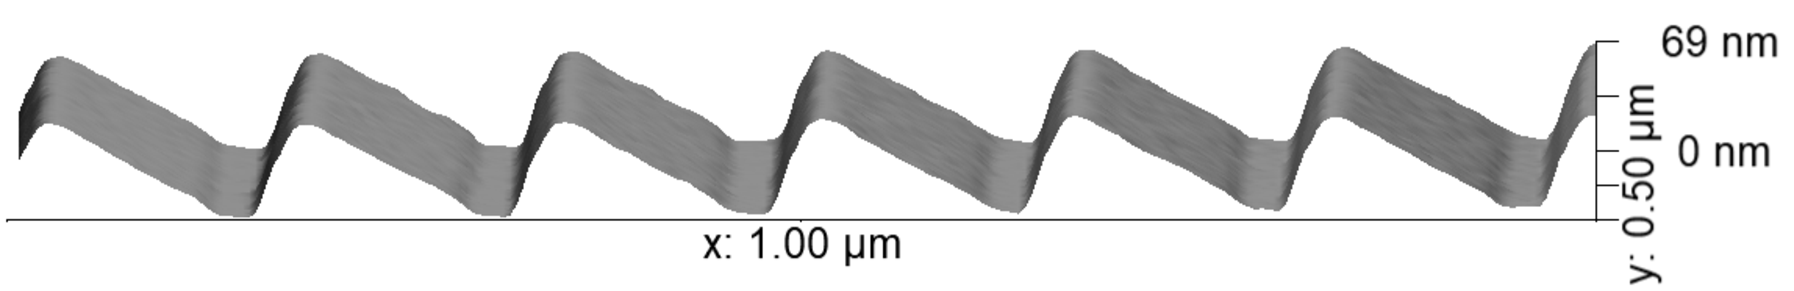
\includegraphics[scale=0.52]{Chapter-4/Figures/AFM_coated.pdf}
 \caption[AFM of a SCIL imprint sputter-coated with \SI{15}{\nm} of gold, using \SI{5}{\nm} of chromium as an adhesion layer.]{AFM of the SCIL imprint shown in \cref{fig:SCIL_AFMs}, sputter-coated with \SI{15}{\nm} of gold, using \SI{5}{\nm} of chromium as an adhesion layer. Following this deposition, facet roughness and blaze angle under AFM measure $\sigma \approx \SI{0.8}{\nm}$ RMS and $28.4 \pm 0.8^{\circ}$, respectively \cite{McCoy17,McCoy20b}.}\label{fig:SCILcoat_AFM} 
 \end{figure}
Using $\zeta \approx 1.7^{\circ}$, a measured facet roughness of $\sigma \approx \SI{0.8}{\nm}$ RMS\footnote{This offers improvement over what is observed in the corresponding UV-NIL imprint, where facet roughness measures $\sigma \approx \SI{1.4}{\nm}$ RMS under AFM [\emph{cf.\@} \cref{fig:uv_nil_AFM}].} and data for $\tilde{\nu}$ obtained from CXRO, $\mathcal{R}_{\text{slab}}$ is also plotted as a function of $\mathcal{E}_{\gamma}$ in \cref{fig:reflectivity}, where it is seen that $\sim \SI{65}{\percent}$ reflectivity is maintained across the test bandpass of \SIrange{400}{900}{\electronvolt}. 
Following the deposition of this coating, the blaze angle under AFM measures $\delta ' = 28.4 \pm 0.8^{\circ}$ from \num{30} individual measurements, which is consistent with the pre-coating measurement of $\delta ' = 27.9 \pm 0.7^{\circ}$. 
The statistical consistency between these two measurements suggests that coating effects had a minimal impact on the blaze angle and that $\delta' / \delta$ constrained from diffraction-efficiency testing results is expected to be indicative of resist shrinkage alone. 

\subsection{Constraining Grating Geometry}\label{sec:grat_geo_scil}
%%%%%%%%%%%%%%%%%%%%%%%%%%%%%%%%%%%%%%%%%--------------------------------------------------
Following the test procedure outlined in \cref{sec:geo_constrain}, near-Littrow configurations for both the silicon master and the coated SCIL replica were established at the beamline using the principal-axis rotations illustrated in \cref{fig:grating_angles}. 
These two gratings were installed one at a time on the optic mount [\emph{cf.\@} \cref{fig:beamline_photoB}] with $\eta \approx 0$ and $\phi \approx 0$ verified by the tilt of the optic mount using a spirit level. 
The groove direction was in each case approximately aligned with the beam direction with $\varphi \approx 0$ so that the $(x',y',z')$ chamber coordinate system [\emph{cf.\@} \cref{fig:beamline_photoA}] is roughly coincident with the $(x,y,z)$ grating coordinate system [\emph{cf.\@} \cref{fig:grating_angles}]. 
In this configuration, the tested grating was carefully adjusted to occult the beam so as to position the point of interception close to the hub of rotation axes. 
With the $\lessapprox \SI{0.5}{\mm}$ cross-sectional diameter of the beam projecting to tens of \si{\mm} at grazing incidence and the point of incidence being the central grooved region of each grating, the effective groove spacing for both gratings was taken as $d = \SI{159.125}{\nm}$, which is the nominal average of the silicon master variable-line-space profile [\emph{cf.\@} \cref{sec:master_for_SCIL}]. 

The detector used for this test campaign was a gallium-arsenide-phosphide Schottky photodiode with a square, \SI{4.6}{\mm} by \SI{4.6}{\mm} collecting area (\textsc{Hamamatsu Photonics}). 
For a grating installed in such an extreme off-plane mount, the linear stage movement of the detector is roughly parallel with the grating-dispersion direction so that each propagating order is confined along an arc with a radius $r = L \sin \left( \gamma \right)$ while being dispersed from $0^{\text{th}}$ order over a horizontal distance given by \cref{eq:disp_approx}, which neglects focal plane corrections on the order of tens of \si{\um} for a fixed value of $L \approx \SI{235}{\mm}$ [\emph{cf.\@} \cref{sec:geo_constrain}]. 
Because the horizontal spacing between each order, $\lambda L / d$, is smaller than the length of this detecting area, $\ell_{\text{det}} = \SI{4.6}{\mm}$, for $d \lessapprox \SI{160}{\nm}$ and $\lambda$ characteristic of soft x-rays, a vertical, \SI{0.5}{\mm}-wide slit was installed to mask this detector so as to allow the intensity of each order, $\mathcal{I}_n \! \left( \lambda \right)$, to be measured in isolation with horizontal stage motion [\emph{cf.\@} \cref{sec:geo_constrain}].  
This is shown in \cref{fig:beamline_photoB}, which depicts a grating installed on the optic mount and the masked detector in the background, with the slit aligned with the goniometric $y'$-direction. 
Because $\ell_{\text{det}} = \SI{4.6}{\mm}$ is also smaller than the expected diffracted-arc radius of $r \approx \SI{7}{\mm}$ for $\gamma \approx 1.7^{\circ}$, however, it is not possible to measure all propagating orders consistently using purely horizontal detector stage motion. 
While measuring diffraction efficiency in this way prevents total diffraction efficiency, $\mathscr{E}_{\text{tot}}$, defined as $\sum_n \mathscr{E}_n$ for $n \neq 0$ [\emph{cf.\@} \cref{sec:measure_efficiency}], from being determined experimentally, it does allow for peak orders to be constrained and compared to theoretical models. 

Described at the start of \cref{sec:beamline_testing}, the nominal value for $\eta$ in a Littrow configuration consistent with $\gamma \approx 1.7^{\circ}$ and $\alpha = \delta = 29.5^{\circ}$ is $\eta \approx 1.5^{\circ}$ by \cref{eq:graze_angle}. 
Thus, with the leveled grating intercepting the beam, the optic mount was rotated about the $x$-axis at the point of incidence to ensure that the angle between the direct beam and the reflected beam was roughly $2 \eta \approx 3^{\circ}$ as measured by the detector as it scans goniometrically in the vertical direction at the location of $0^{\text{th}}$ order. 
Starting with this basic configuration for each tested grating, small adjustments to $\eta$ and $\varphi$ were made while the arc of diffraction was analyzed in-situ after being mapped as a function of $x$ and $y$ to confirm a near-Littrow configuration. 
Unlike the $x$-positions of propagating orders given by \cref{eq:disp_approx}, which can be measured directly by scanning the detector linearly along the horizontal direction and then calculating weighted-mean centroids [\emph{cf.\@} \cref{fig:ALS_xdata}], their corresponding $y$-positions require precise knowledge of the system throw, $L \approx \SI{235}{\mm}$, to map the goniometric angle associated with vertical stage motion, $\Theta_n$, to a linear $y$-coordinate using $y_n = L \sin \left( \Theta_n \right)$ [\emph{cf.\@} \cref{sec:geo_constrain}]. 

The quantity $L$ was experimentally determined separately for each installed grating by comparing $\ell_{\text{det}}$ to the angular size of the detector as measured by a goniometric scan of the beam at the location of $0^{\text{th}}$ order [\emph{cf.\@} \cref{fig:ALS_cent_throw}]. 
\begin{figure}
 \centering
 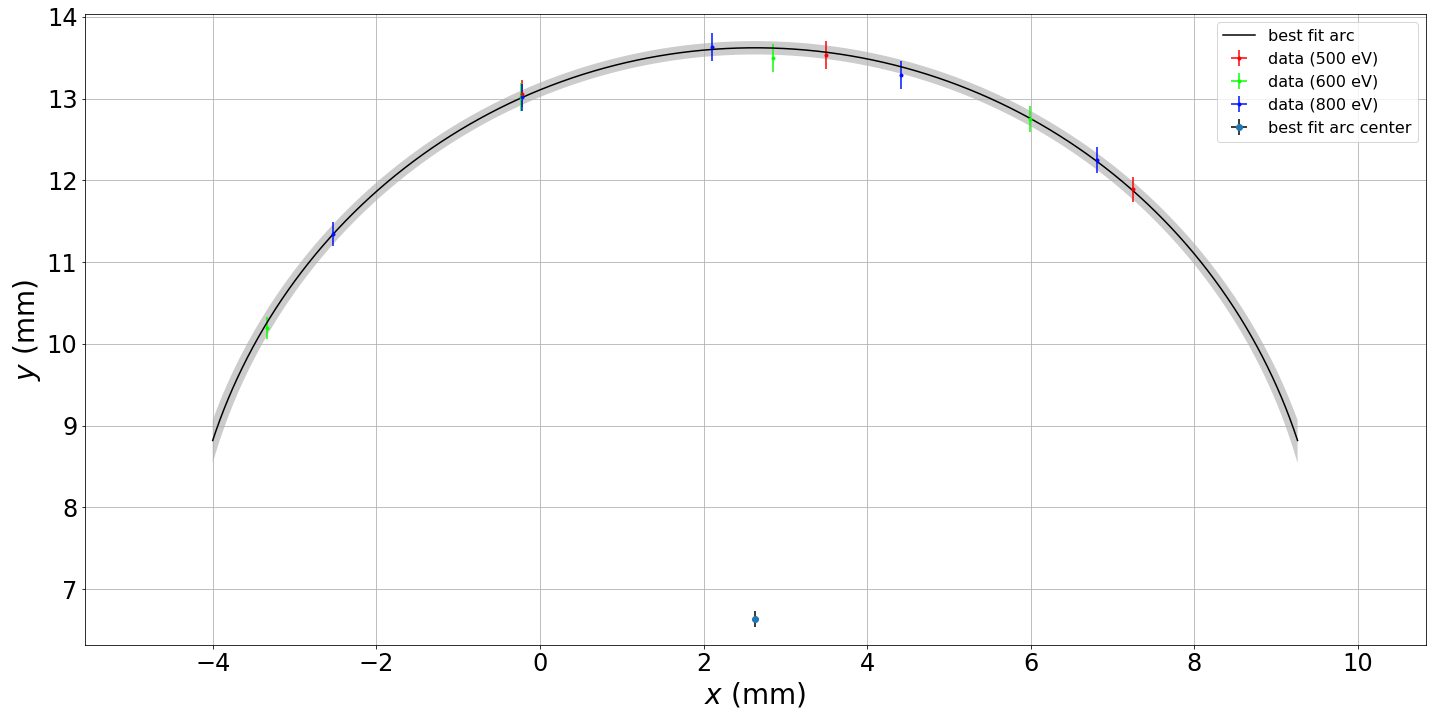
\includegraphics[scale=0.31]{Chapter-4/Figures/arc_fit_alt_si.png}
 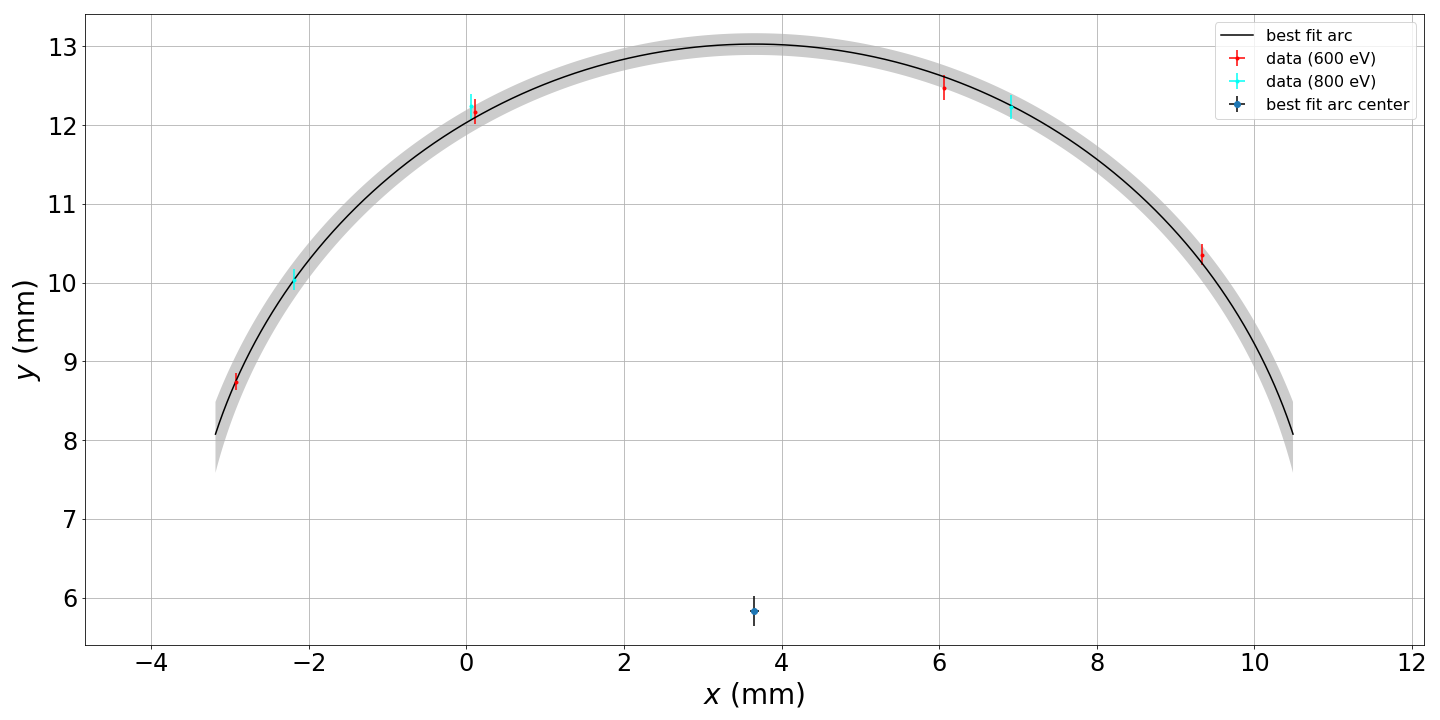
\includegraphics[scale=0.31]{Chapter-4/Figures/arc_fit_alt_scil.png}
 \caption[Measured diffracted arcs for the silicon master and the coated SCIL replica]{Measured diffracted arcs for the silicon master (\emph{top}) and the coated SCIL replica (\emph{bottom}) in their respective test configurations, fit to half-circles. Grayed regions represent one standard deviation uncertainty \cite{McCoy20b}.}\label{fig:arc_fit}
 \end{figure}
This allowed $r$ to be inferred from fitting measured $(x,y)$ data, gathered at a few photon energies, to a half circle, which is shown in \cref{fig:arc_fit} for both the silicon master and the coated SCIL replica. 
The angle $\gamma$ for each grating was then determined from $\sin \left( \gamma \right) = r/ L$ [\emph{cf.\@} \cref{eq:arc_radius}] before the remaining angles were calculated using the fit values for the arc center coordinates as they compare to the measured $(x,y)$ locations of $0^{\text{th}}$ order as well as the direct beam. 
First, the angle $\alpha$ was measured using \cref{eq:measure_alpha} and similarly, the grating roll characterized by the angle $\phi$ was constrained through \cref{eq:measure_roll} [\emph{cf.\@} \cref{fig:ALS_arc}]. 
With this value for $\phi$ and a measured $y$-distance between $0^{\text{th}}$ order and the center of the diffracted arc, $\Delta y_0$, the substrate graze angle, $\eta$, was measured for each grating using \cref{eq:measure_graze} before grating yaw, which is parameterized by the angle $\varphi$, was determined from \cref{eq:measure_yaw}. 
\begin{table}[]
 \centering
 \caption[Measured diffracted-arc parameters for the silicon master and the coated SCIL replica in their respective test configurations at the ALS]{Measured diffracted-arc parameters for the silicon master and the coated SCIL replica in their respective test configurations at the ALS \cite{McCoy20b}.}\label{tab:arc_params}
 \begin{tabular}{cccc}
 \cline{1-3}
 measured parameter                                                     & \ master         		  & \ replica     \\ \hline
 $L$                                    & \ $234.7 \pm \SI{3.0}{\mm}$   & \ $235.6 \pm \SI{3.0}{\mm}$ \\
 $r$                                    & \ $6.98 \pm \SI{0.08}{\mm}$   & \ $7.20 \pm \SI{0.14}{\mm}$ \\
 $\Delta x_{\text{dir}}$ 				& \ $2.80 \pm \SI{0.03}{\mm}$   & \ $3.68 \pm \SI{0.07}{\mm}$ \\
 $\Delta x_0$  							& \ $2.86 \pm \SI{0.03}{\mm}$   & \ $3.57 \pm \SI{0.06}{\mm}$ \\
 $\Delta y_0$  							& \ $6.41 \pm \SI{0.10}{\mm}$   & \ $6.34 \pm \SI{0.19}{\mm}$ \\ 
 $\gamma$ by \cref{eq:arc_radius}       & \ $1.71 \pm 0.03^{\circ}$ 	& \ $1.75 \pm 0.04^{\circ}$   \\
 $\alpha$ by \cref{eq:measure_alpha}    & \ $23.7 \pm 0.7^{\circ}$  	& \ $30.7 \pm 0.9^{\circ}$    \\ 
 $\phi$ by \cref{eq:measure_roll}       & \ $0.50 \pm 0.14^{\circ}$ 	& \ $0.98 \pm 0.39^{\circ}$   \\
 $\eta$ by \cref{eq:measure_graze}      & \ $1.57 \pm 0.03^{\circ}$ 	& \ $1.54 \pm 0.05^{\circ}$   \\
 $\varphi$ by \cref{eq:measure_yaw}     & \ $0.68 \pm 0.01^{\circ}$ 	& \ $0.89 \pm 0.02^{\circ}$   \\ \hline
 \end{tabular}
 \end{table}
These measured parameters are listed in \cref{tab:arc_params} for both gratings. %the silicon master and the coated SCIL replica. 

Although the measured values for $\eta$ and $\varphi$ depart slightly from the targeted values of $\eta \approx 1.5^{\circ}$ and $\varphi \approx 0.84^{\circ}$, the arc parameters listed in \cref{tab:arc_params} indicate near-Littrow configurations for both gratings. 
By \cref{eq:blaze_wavelength} for the blaze wavelength, the diffraction efficiency of propagating orders with $n=2$ and $n=3$ are expected to maximize in the spectral range $\SI{440}{\electronvolt} \leq \mathcal{E}_{\gamma} \leq  \SI{900}{\electronvolt}$ for a grating with $d \lessapprox \SI{160}{\nm}$ in a near-Littrow configuration with $\gamma \approx 1.7^{\circ}$. 
Moreover, rewriting \cref{eq:blaze_wavelength} for the blaze wavelength as [\emph{cf.\@} \cref{eq:angle_on_groove,eq:blaze_wavelength_general}]
\begin{subequations}
\begin{equation}\label{eq:blaze_wavelength_alt}
 \lambda_b = \frac{2 d \sin \left( \zeta \right) \sin \left( \delta \right)}{n} = \frac{2 d \sin \left( \gamma \right) \sin \left( \delta \right)}{n} \cos \left( \delta - \alpha \right) 
 \end{equation}
and then invoking small angle approximations for $\gamma$ as well as $\abs{\delta - \alpha}$ gives %in terms of radians
\begin{equation}\label{eq:blaze_wavelength_alt_approx}
 \lambda_b \approx \frac{2 d \gamma \sin \left( \delta \right)}{n} \left( 1 - \frac{\left( \delta - \alpha \right)^2}{2} \right) .
 \end{equation}
\end{subequations}
This approximate expression suggests that the locations of peak orders are most sensitive to $\delta$ and $\gamma$ in an extreme off-plane mount rather than $\alpha$ provided that $\abs{\delta - \alpha} \ll \SI{1}{\radian}$, which describes a near-Littrow configuration. 
With both gratings loosely satisfying this condition for $\alpha$, the grating geometries listed in \cref{tab:arc_params} were employed for testing.

\subsection{Test Results for Diffraction Efficiency}\label{sec:test_results_scil}
%%%%%%%%%%%%%%%%%%%%%%%%%%%%%%%%%%%%%%%%%--------------------------------------------------
Experimental data for $\mathscr{E}_n$ were gathered as a function of $\mathcal{E}_{\gamma}$ over the range \SIrange{440}{900}{\electronvolt} using test configurations defined by the parameters listed in \cref{tab:arc_params}. 
As described in \cref{sec:measure_efficiency} and carried out in \cref{sec:test_results_taste}, $\mathcal{I}_n$ for each propagating order, at each value of $\mathcal{E}_{\gamma}$, was measured using the masked photodiode by scanning the diffracted arc horizontally, in \SI{50}{\um} steps, and then determining the maximum of each diffracted order. 
Meanwhile, $\mathcal{I}_{\text{inc}}$ for the unobstructed beam was measured at each value of $\mathcal{E}_{\gamma}$ in an analogous way, with the grating moved out of the path of the beam. 
The quantity $\mathscr{E}_n$ was then determined through $\mathcal{I}_n / \mathcal{I}_{\text{inc}}$ [\emph{cf.\@} \cref{eq:diffraction_efficiency}] after subtracting dark current as in \cref{sec:test_results_taste}, but due to the use of a detector that is smaller than the radius of the diffracted arc [\emph{cf.\@} \cref{sec:grat_geo_scil}], $\mathcal{I}_n$ measurements for propagating orders near the bottom of the diffracted arc were missed systematically during data collection. 
\begin{figure}
 \centering
 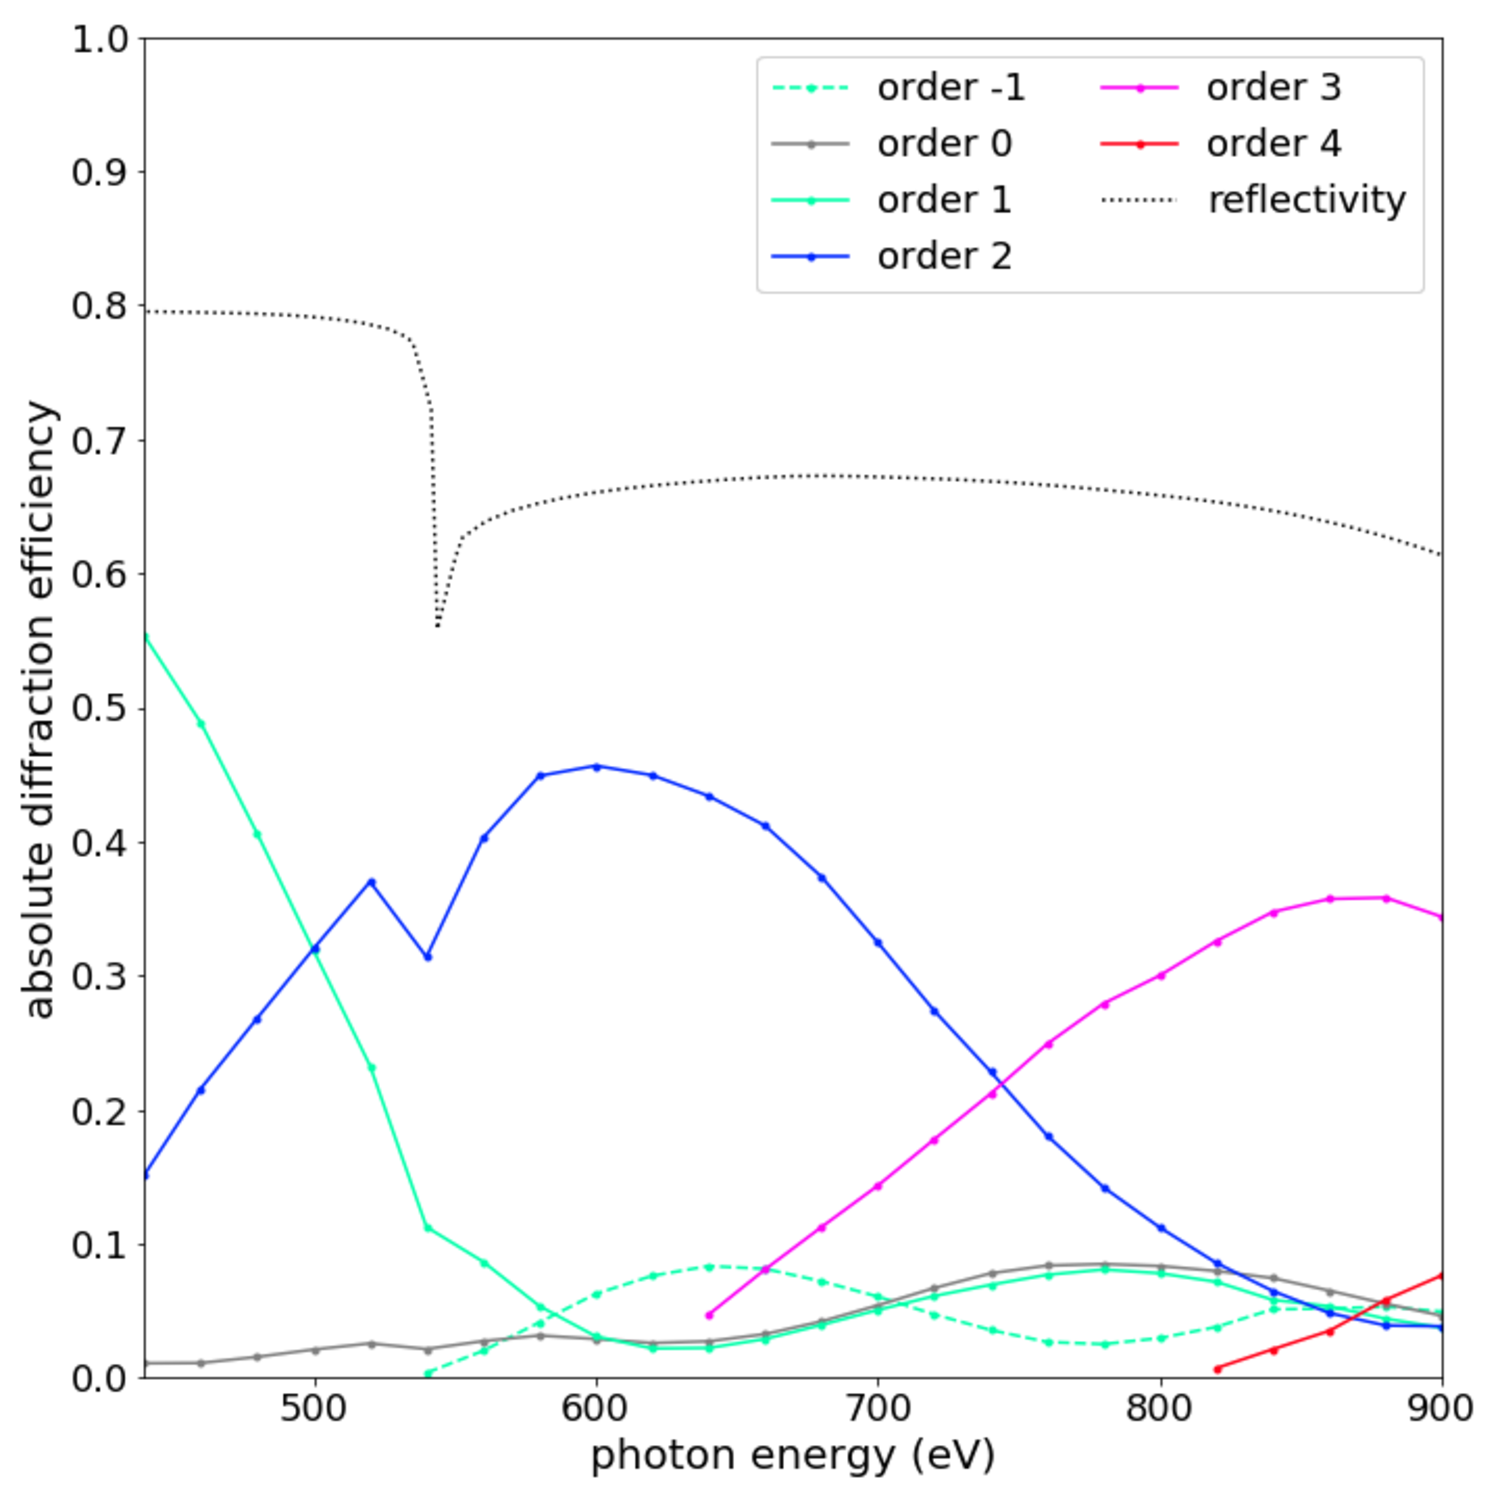
\includegraphics[scale=0.4]{Chapter-4/Figures/si_data.pdf}
 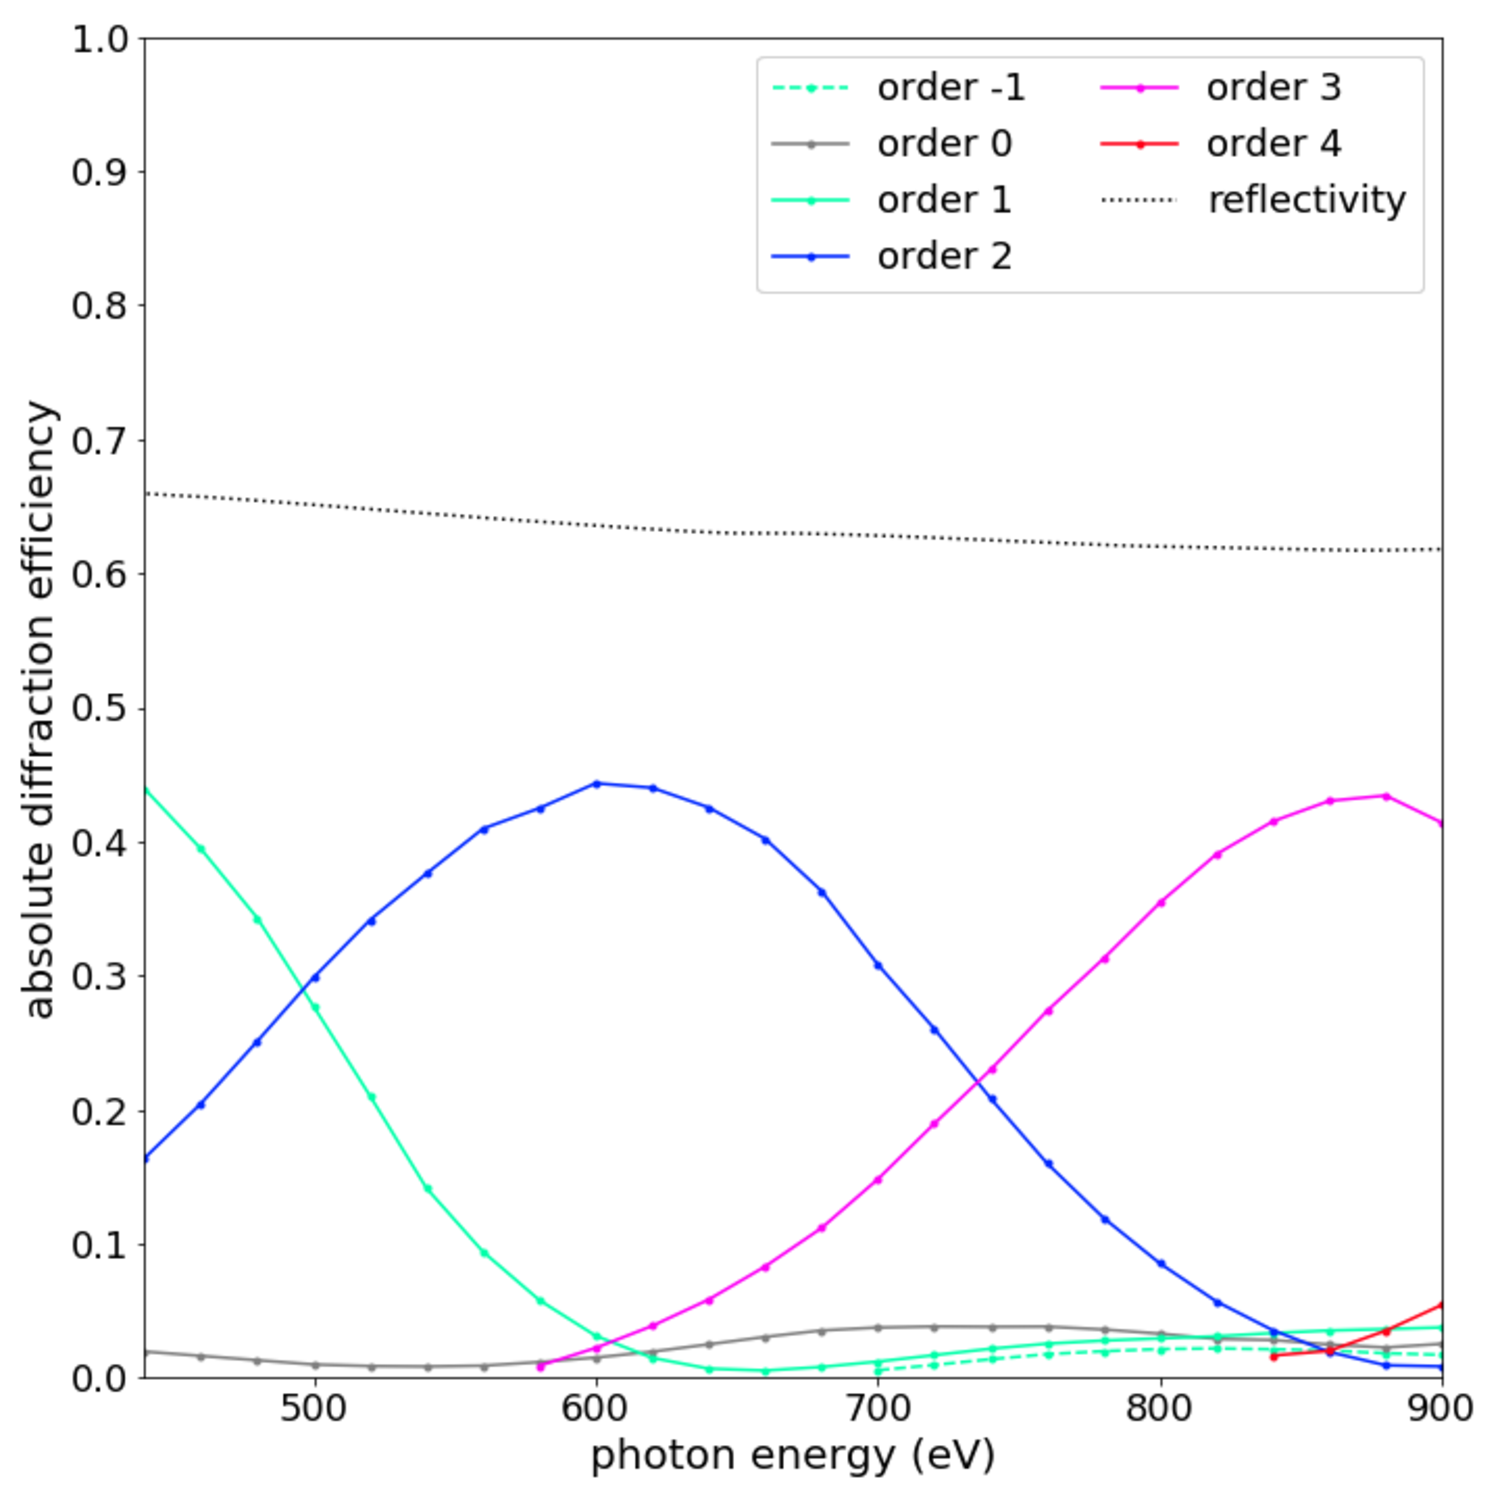
\includegraphics[scale=0.4]{Chapter-4/Figures/scil_data.pdf}
 \caption[Measured absolute diffraction efficiency data for the silicon master and the coated SCIL replica]{Measured absolute diffraction efficiency data for the silicon master (\emph{top}) and the coated SCIL replica (\emph{bottom}) in geometrical configurations described by the parameters listed in \cref{tab:arc_params} compared to specular reflectivity calculated using the parameters listed in \cref{tab:nom_params} \cite{McCoy20b}.}\label{fig:abs_eff}
 \end{figure} 
Notwithstanding this, $\mathscr{E}_n$ was measured every \SI{20}{\electronvolt} between \SI{440}{\electronvolt} and \SI{900}{\electronvolt}; these results are plotted in \cref{fig:abs_eff} for both gratings. %the silicon master and the SCIL replica. 

The data plotted in \cref{fig:abs_eff} are compared to specular reflectivity curves relevant for each case, which are plotted as dotted lines. 
\begin{table}[]
 \centering
 \caption[Nominal parameters relevant for specular reflectivity analysis and diffraction-efficiency modeling of the silicon master and the coated SCIL replica ]{Nominal parameters relevant for specular reflectivity analysis and diffraction-efficiency modeling of the silicon master and the coated SCIL replica \cite{McCoy20b}.}\label{tab:nom_params} 
 \begin{tabular}{cccc}
 \cline{1-3}
 nominal parameter                                  & \ master         		  								  & \ replica            \\ \hline
 $\gamma$											& $1.71^{\circ}$								  		  & $1.75^{\circ}$	 	 \\
 $\alpha$											& $23.7^{\circ}$								          & $30.7^{\circ}$	 	 \\
 estimated blaze angle ($\delta$, $\delta'$) 		& $29.5^{\circ}$								  		  & $28^{\circ}$	 	 \\
 blaze angle by AFM ($\delta$, $\delta'$) 			& $30.0^{\circ}$								  		  & $28.4^{\circ}$	 	 \\
 facet incidence angle ($\zeta$) 					& $1.70^{\circ}$								          & $1.75^{\circ}$	 	 \\
 reflective material 								& \SI{3}{\nm} \ce{SiO2} on \ce{Si}						 & \ce{Au} (thick slab)		 \\
 eq.\ for specular reflectivity 					& \cref{eq:Si_layer_refl} with \cref{eq:NC_factors} & \cref{eq:Au_refl} \\
 facet roughness ($\sigma$)							& $\SI{0.4}{\nm}$ RMS						  			  & $\SI{0.8}{\nm}$ RMS	 	 \\ \hline
 \end{tabular}
 \end{table}
Summarized in \cref{tab:nom_params}, these curves were calculated according to the considerations outlined in \cref{sec:reflectivity} but with updated values for the facet-incidence angle, $\zeta$, which follow from the nominal values for $\gamma$ and $\alpha$ as well as the expected blaze angles, $\delta$ and $\delta'$. 
Peak-order values of $\mathscr{E}_n$ range from \SIrange{40}{45}{\percent} for both gratings or equivalently, \SIrange{65}{70}{\percent} measured relative to the reflectivity in each case, which is comparable to the results reported for the corresponding UV-NIL replica presented by Miles, et~al.~\cite{Miles18}. 
However, because not all diffracted orders are accounted for due to the condition $\ell_{\text{det}} < r$, $\mathscr{E}_{\text{tot}}$ is not plotted in \cref{fig:abs_eff} [\emph{cf.\@} \cref{sec:geo_constrain}]. 

\section{Analysis and Discussion}\label{sec:discussion_scil}
%%%%%%%%%%%%%%%%%%%%%%%%%%%%%%%%%%%%%%%%%--------------------------------------------------
The soft x-ray diffraction-efficiency measurements presented in \cref{sec:test_results_scil} demonstrate that both the silicon master and the corresponding SCIL replica exhibit a significant blaze response in a near-Littrow, grazing-incidence configuration. 
Using these data, the following analysis seeks to constrain the impact of resist shrinkage on the blaze angle of the SCIL replica by estimating $\delta' / \delta$ through comparing measured single-order efficiency curves to those predicted by theoretical models of diffraction efficiency. 
The models utilized for this study were produced with the aid of the software package \textsc{PCGrate-SX} (v.\ 6.1) \cite{PCGrate_web}, which solves the Helmholtz equation through the integral method for a custom grating boundary and incidence angles input by the user \cite[\emph{cf.\@} \cref{sec:grat_bound_consider}]{Goray10}. 
In each case, the grating boundary is taken to be perfectly conducting so that the electromagnetic fields inside the grating material are null. 
While this implies lossless diffraction efficiency for a perfectly smooth grating boundary as shown in \cref{sec:rel_eff_perf}, the overall response is modulated by the appropriate specular reflectivity in each case [\emph{cf.\@} \cref{sec:reflectivity,sec:refl_account}]. 
The incident radiation is treated as having a wave vector given by \cref{eq:beam_vec_grat} and \emph{TE polarization} [\emph{cf.\@} \cref{fig:polarization_angle}] for the reasons outlined in \cref{sec:grat_bound_consider}.  
Additionally, the absorbing effect surface roughness in the limit of small surface features is taken into account by using the appropriate Nevot-Croce factors [\emph{cf.\@} \cref{eq:NC_factors}] with the values for facet roughness listed in \cref{tab:nom_params}.  
The groove spacing in each case is assumed to be $d = \SI{159.125}{\nm}$ based on the considerations outlined in \cref{sec:grat_geo_scil}.
With \cref{sec:silicon_master_sub,sec:scil_replica_sub} treating the silicon master and the SCIL replica, respectively, \cref{sec:shrinkage_model} presents an approximate model for resist shrinkage based on simple geometric considerations to interpret this result. 

\subsection{Silicon Master}\label{sec:silicon_master_sub}
%%%%%%%%%%%%%%%%%%%%%%%%%%%%%%%%%%%%%%%%%--------------------------------------------------
As a point of reference for evaluating resist shrinkage in the SCIL replica, the diffraction-efficiency results for the silicon master [\emph{cf.\@} \cref{fig:abs_eff}, \emph{top panel}] are compared to \textsc{PCGrate-SX} models in \cref{fig:model_si1}. 
\begin{figure}
 \centering
 %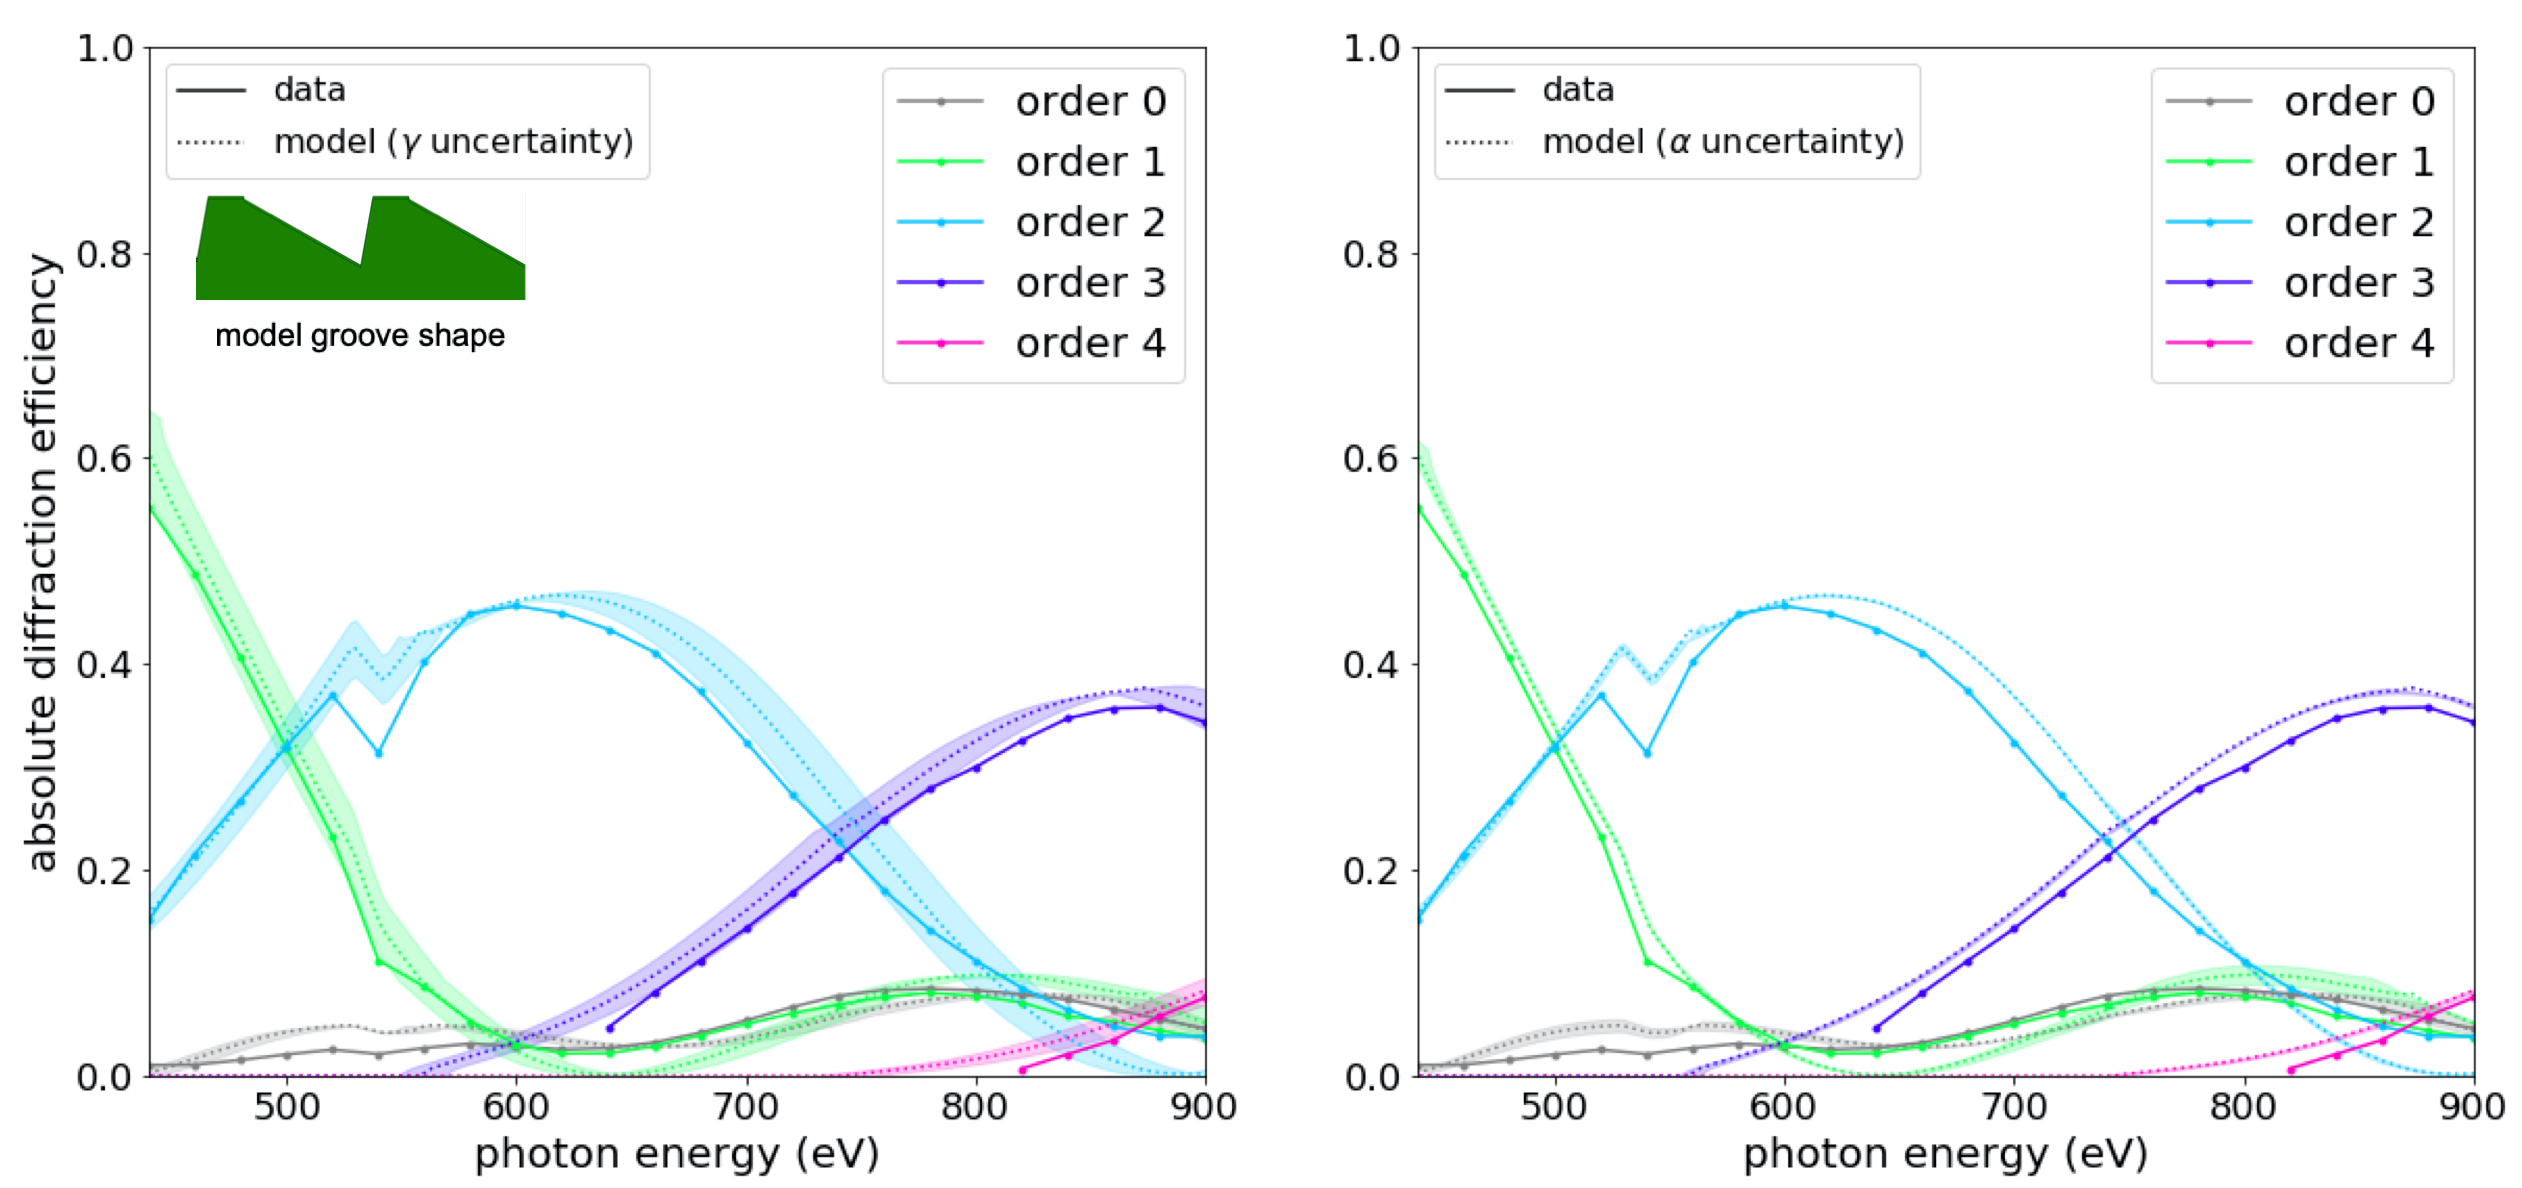
\includegraphics[scale=0.37]{Chapter-4/Figures/si_double1.pdf}
 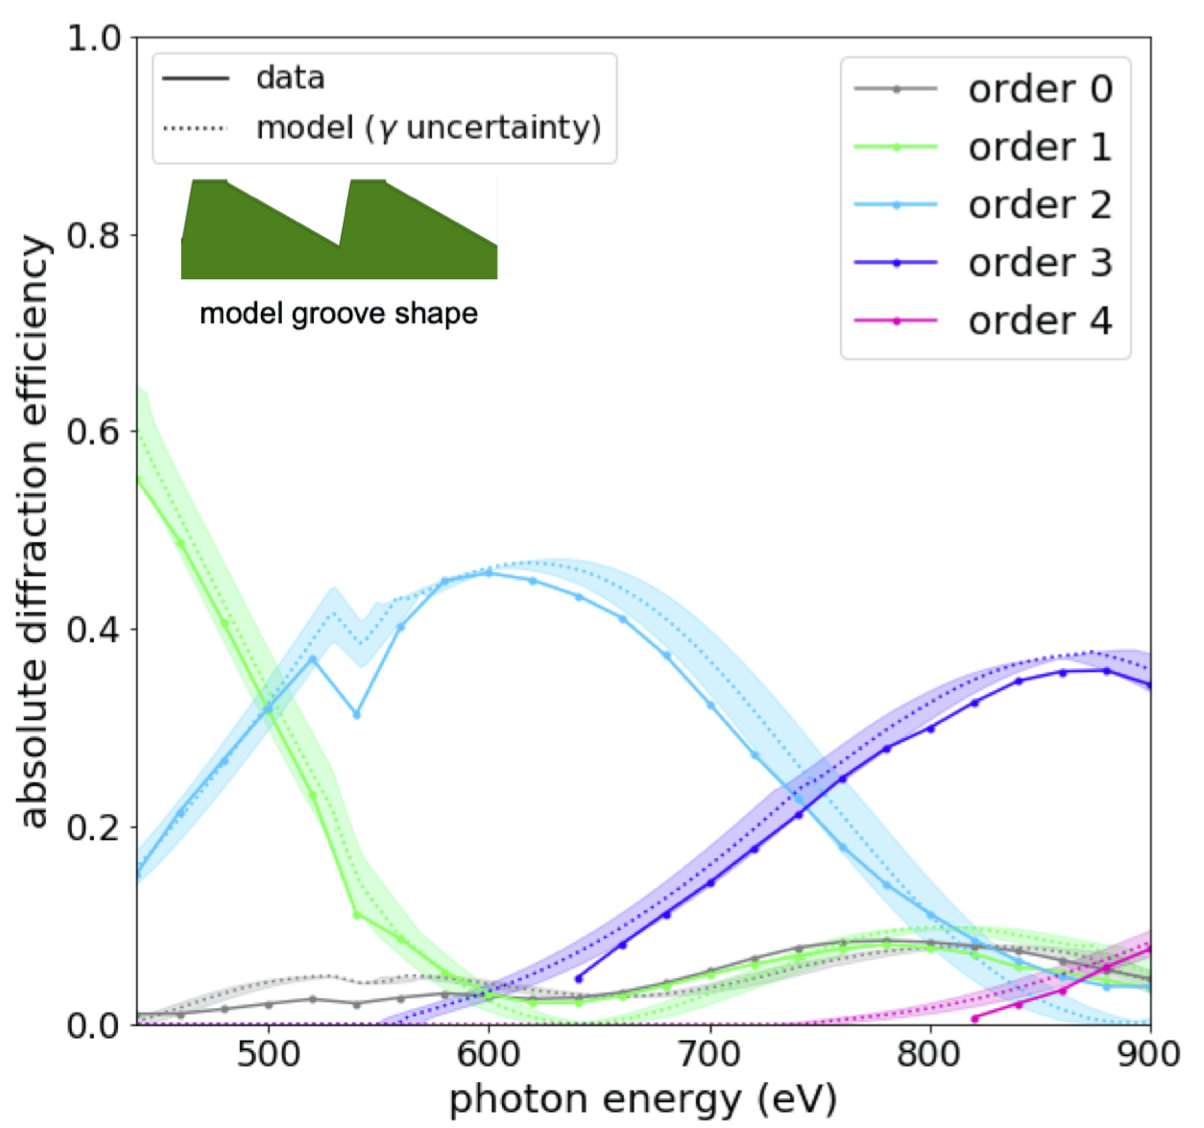
\includegraphics[scale=0.25]{Chapter-4/Figures/si_double1_a.png}
 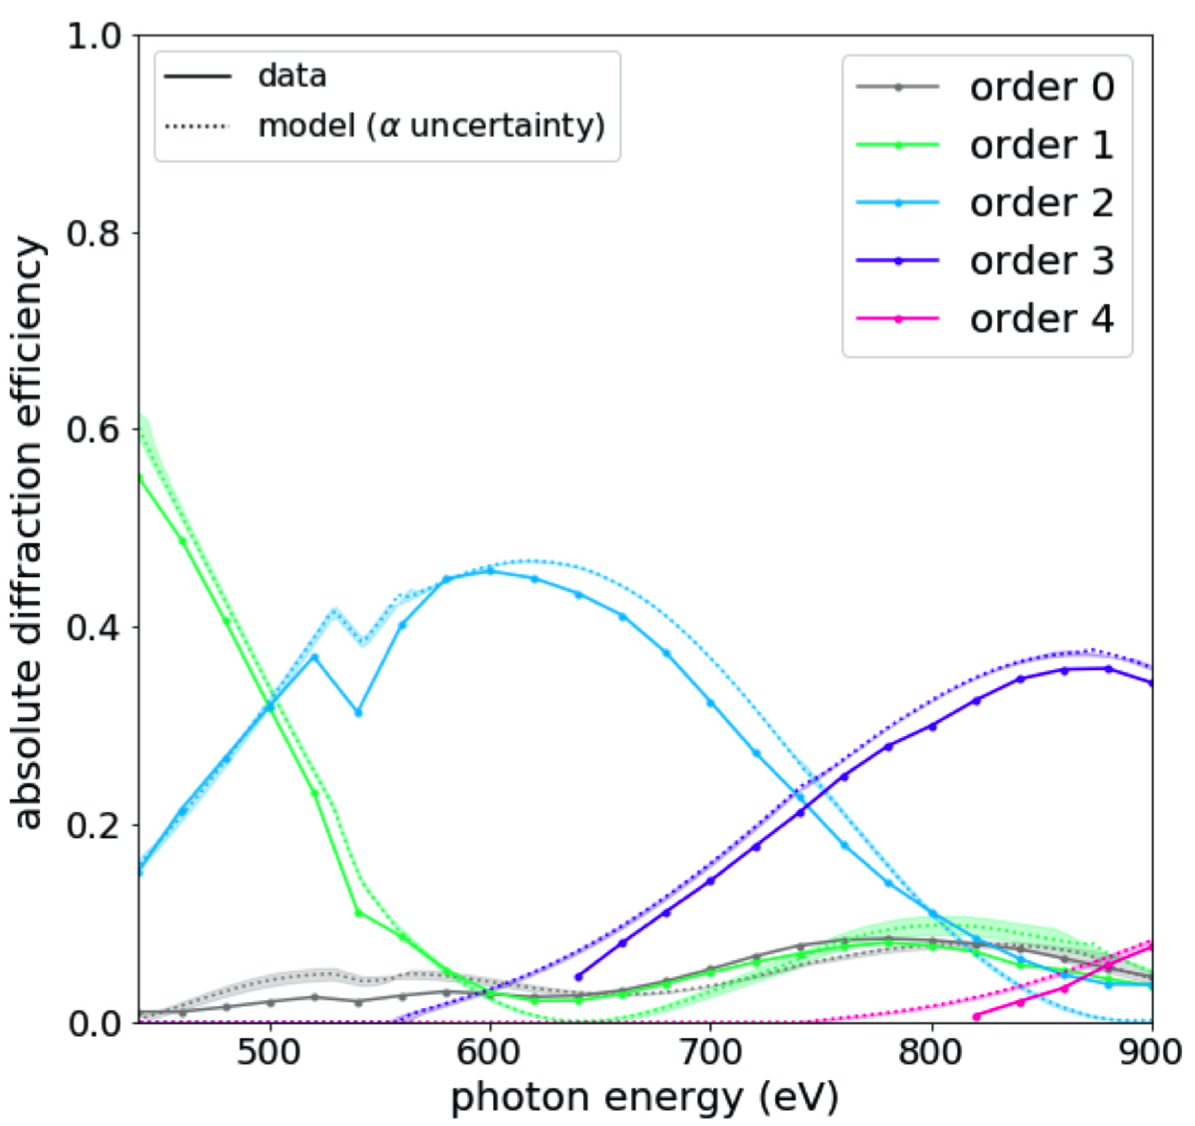
\includegraphics[scale=0.25]{Chapter-4/Figures/si_double1_b.png}
 \caption[Measured absolute diffraction efficiency data for the silicon master compared to \textsc{PCGrate-SX} models that assume a groove profile similar to a \ce{KOH}-etched $\langle 311 \rangle$ silicon grating]{Measured absolute diffraction efficiency data for the silicon master [\emph{cf.\@} \cref{fig:abs_eff}, \emph{top panel}] compared to \textsc{PCGrate-SX} models that assume a groove profile similar to a \ce{KOH}-etched $\langle 311 \rangle$ silicon grating with $\delta = 29.5^{\circ}$, $\bar{\delta} \approx 80^{\circ}$, and a grove depth of $h \approx \SI{67}{\nm}$ with $w = \SI{35}{\nm}$ and $\Delta h = \SI{3}{\nm}$ [\emph{cf.\@} \cref{eq:groove_depth}]. In the top and bottom panels, respectively, $\gamma$ and $\alpha$ are allowed to vary at levels of $1.71 \pm 0.03^{\circ}$ and $23.7 \pm 0.7^{\circ}$ (\emph{shaded swaths}) \cite{McCoy20b}.}\label{fig:model_si1}
 \end{figure} 
These models are based on the wet-etched grating topography described in \cref{sec:master_for_SCIL} together with incident radiation parameterized by $\gamma$ and $\alpha$ for the test-configuration geometry established in \cref{sec:grat_geo_scil}. %in \cref{sec:crystal_etching} 
The grating boundary is defined using the trapezoid-like groove shape shown in the figure inset, with nominal sawtooth angles of $\delta = 29.5^{\circ}$ and $\bar{\delta} \approx 80^{\circ}$ for $\langle 311 \rangle$-oriented, \ce{KOH}-etched silicon [\emph{cf.\@} \cref{tab:off_axis_si}], a flat-top width of $w = \SI{35}{\nm}$, a nub-protrusion height of $\Delta h = \SI{3}{\nm}$ and a groove depth of $h \approx \SI{67}{\nm}$ [\emph{cf.\@} \cref{eq:groove_depth}]. %[\emph{cf.\@} \cref{fig:master_grating_profile}]
In both panels of \cref{fig:model_si1}, the model corresponding to the nominal values $\gamma = 1.71^{\circ}$ and $\alpha = 23.7^{\circ}$ [\emph{cf.\@} \cref{tab:nom_params}] is plotted as a series of dotted lines for each diffracted order shown. 
Models that take into account the uncertainties for $\gamma$ and $\alpha$ listed in \cref{tab:arc_params} are then plotted as shaded swaths in the top and bottom panels of \cref{fig:model_si1}, respectively. 

The results presented in \cref{fig:model_si1} show that the geometry constrained in \cref{sec:grat_geo_scil} leads to the production of models that roughly match the experimental data. 
Mismatches between the models and the data may be in part due to the detailed shape of nubs atop of each groove, which cannot be described with a functional form\footnote{This refers to the periodic groove function, $g(x)$, defined in \cref{sec:grating_boundary}.} due to the presence of a small, indented sidewall [\emph{cf.\@} \cref{fig:master_grating_profile,fig:master_grating_SEM}]. % as illustrated in \cref{fig:master_grating_profile} and shown under FESEM in \cref{fig:master_grating_SEM}. 
Although this limits the accuracy of the \textsc{PCGrate-SX} models utilized, the model uncertainty swaths indicate that $\gamma$ serves to shift the centroids of peak orders\footnote{\emph{i.e.}, the photon-energy equivalent to the blaze wavelength, $h c_0 / \lambda_b$} while $\alpha$ has a relatively small impact as expected from \cref{eq:blaze_wavelength_alt_approx}. 
\begin{figure}
 \centering
 %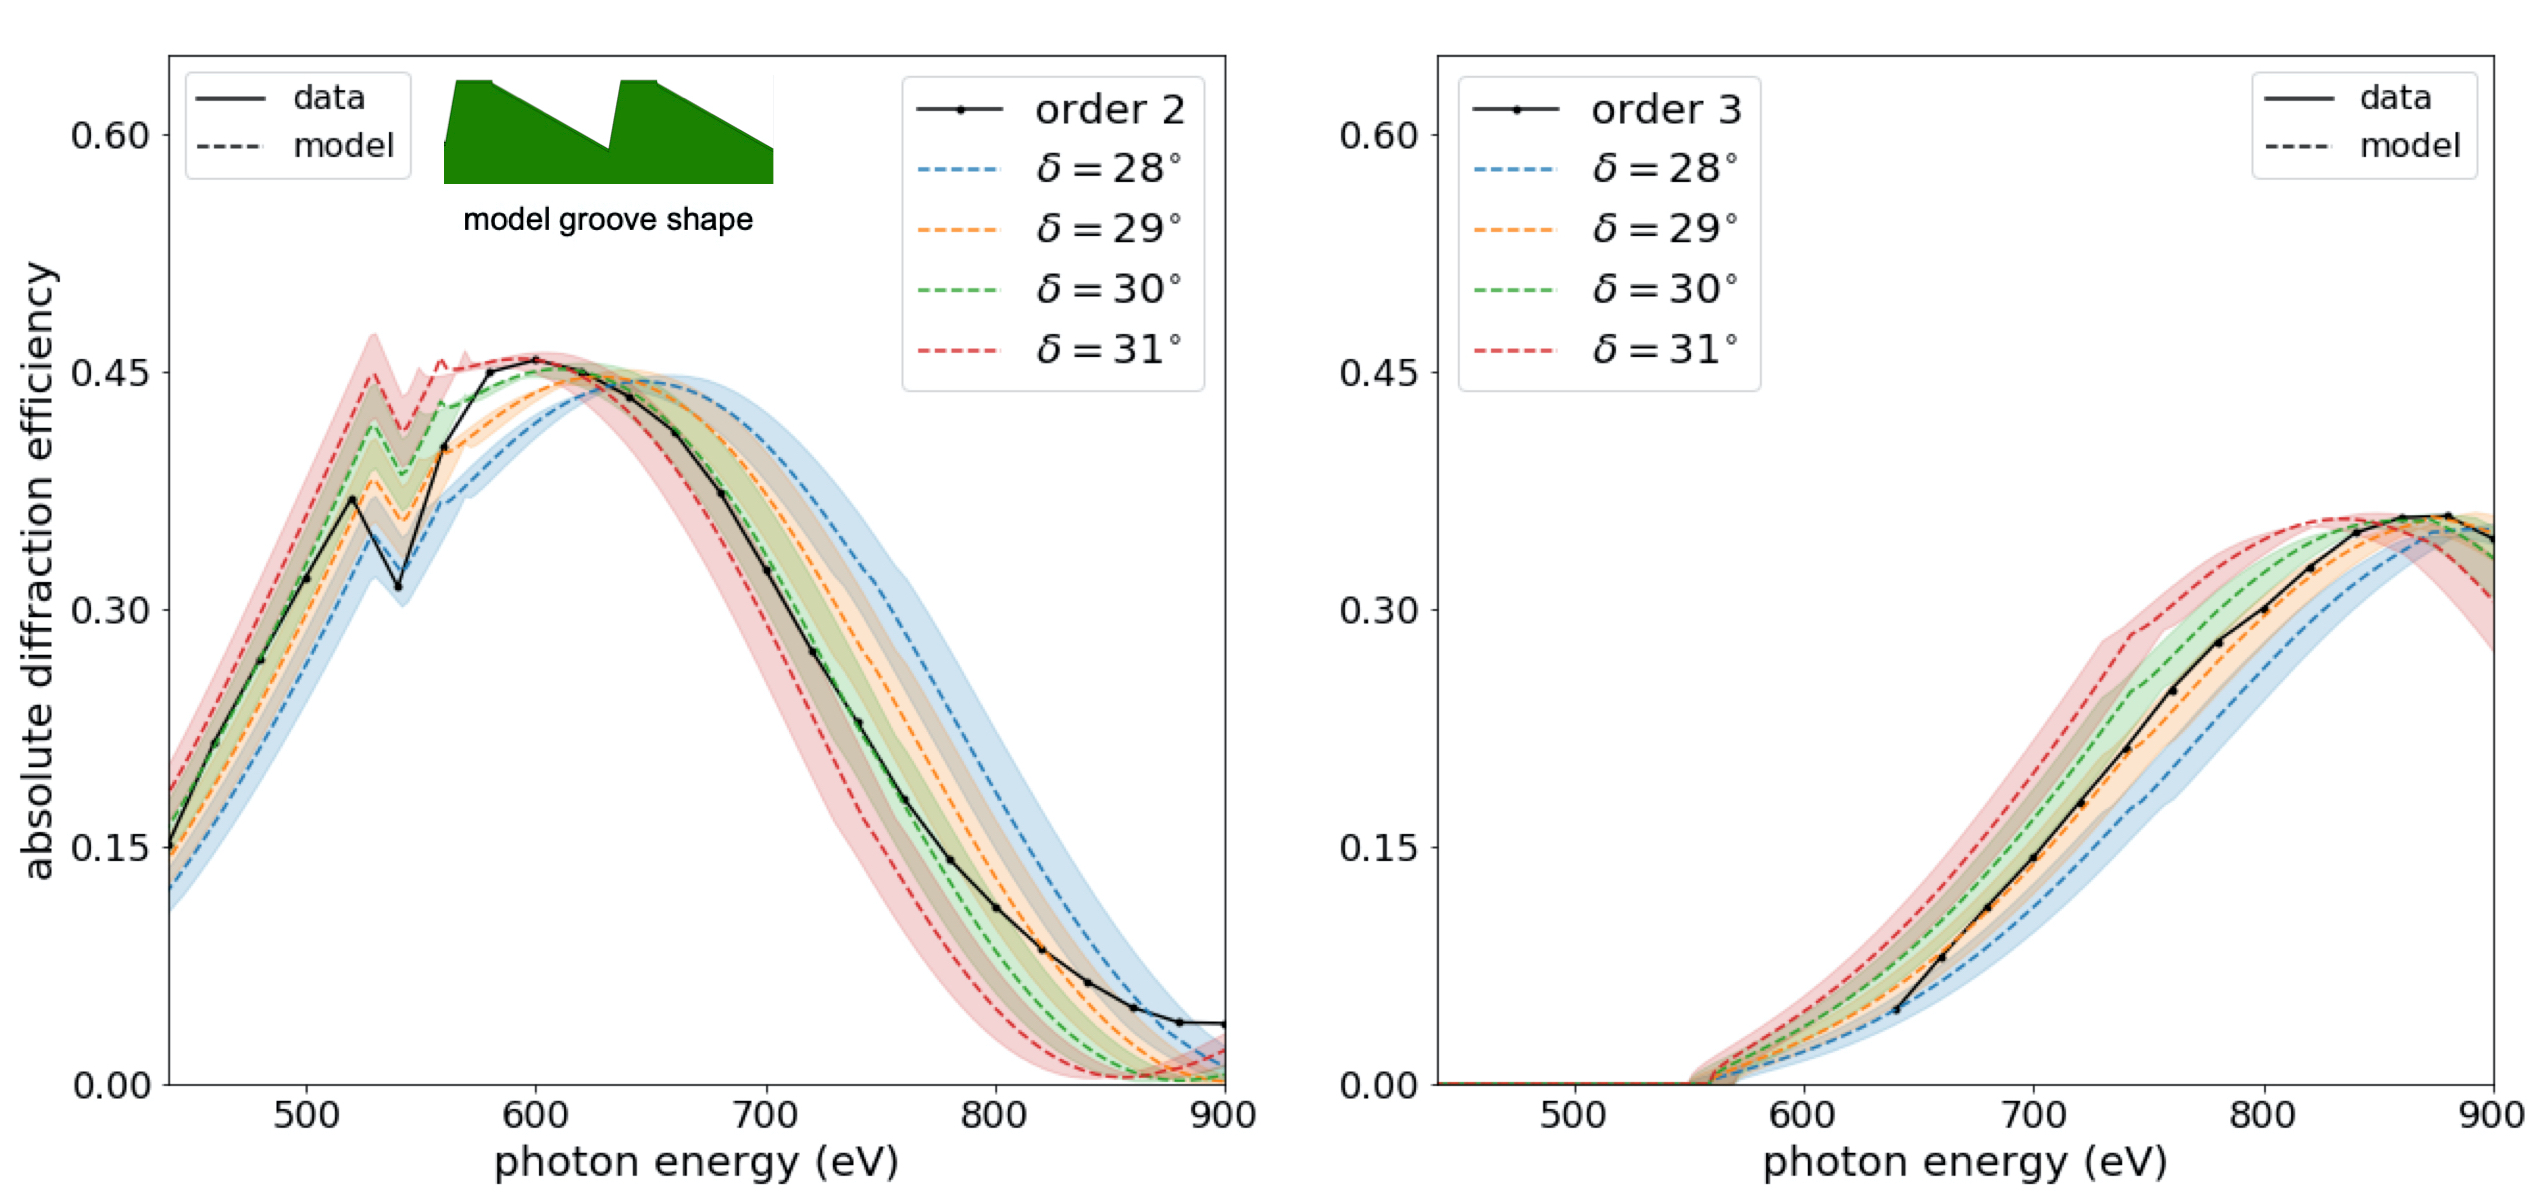
\includegraphics[scale=0.37]{Chapter-4/Figures/si_double2.pdf}
 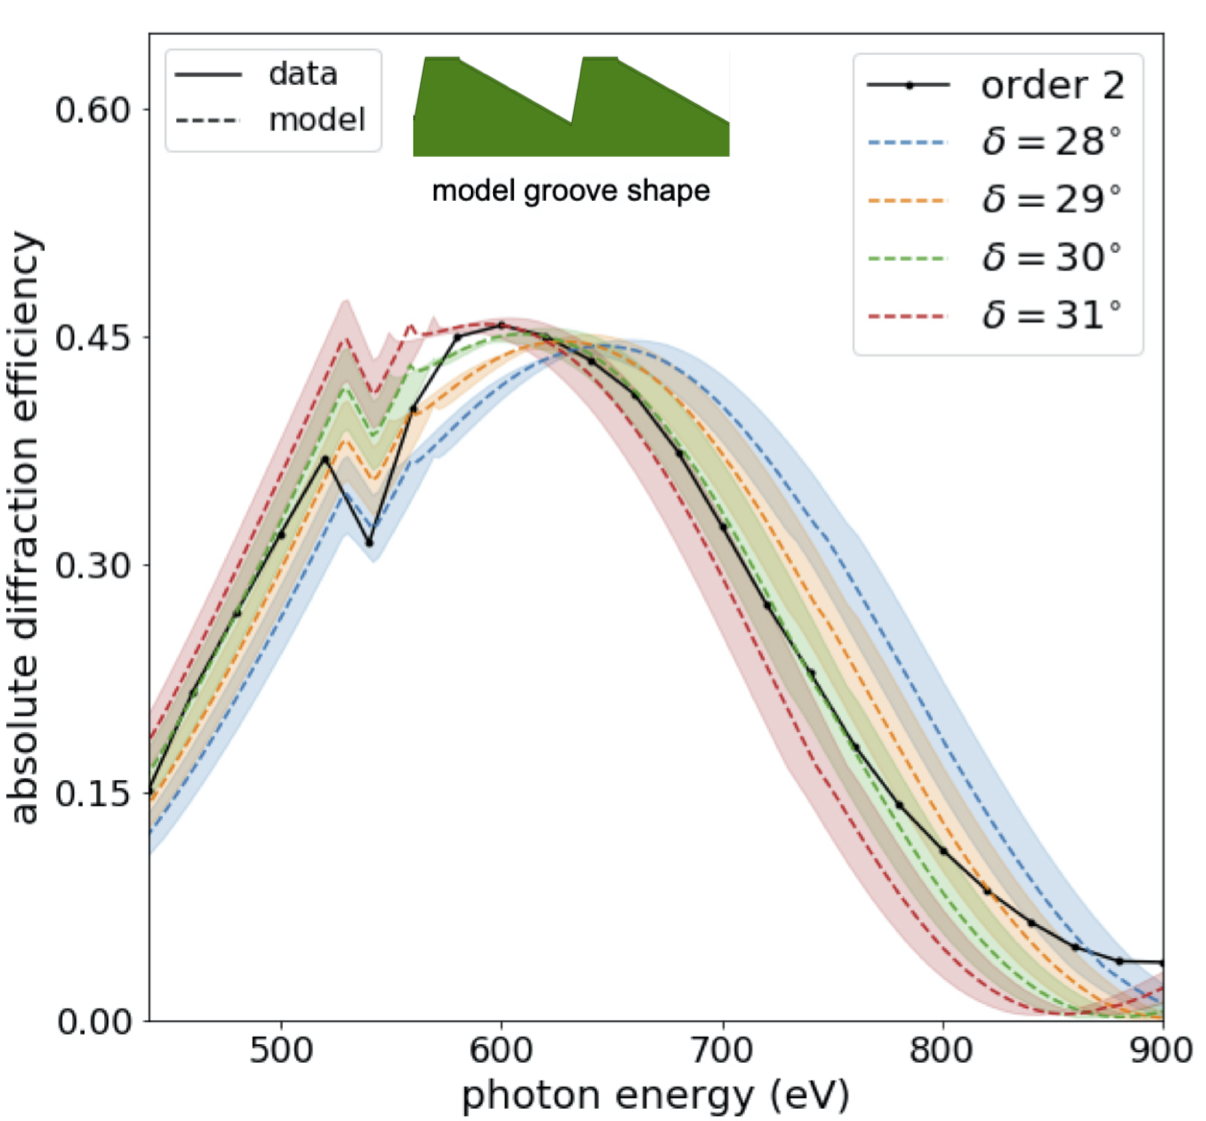
\includegraphics[scale=0.25]{Chapter-4/Figures/si_double2_a.png}
 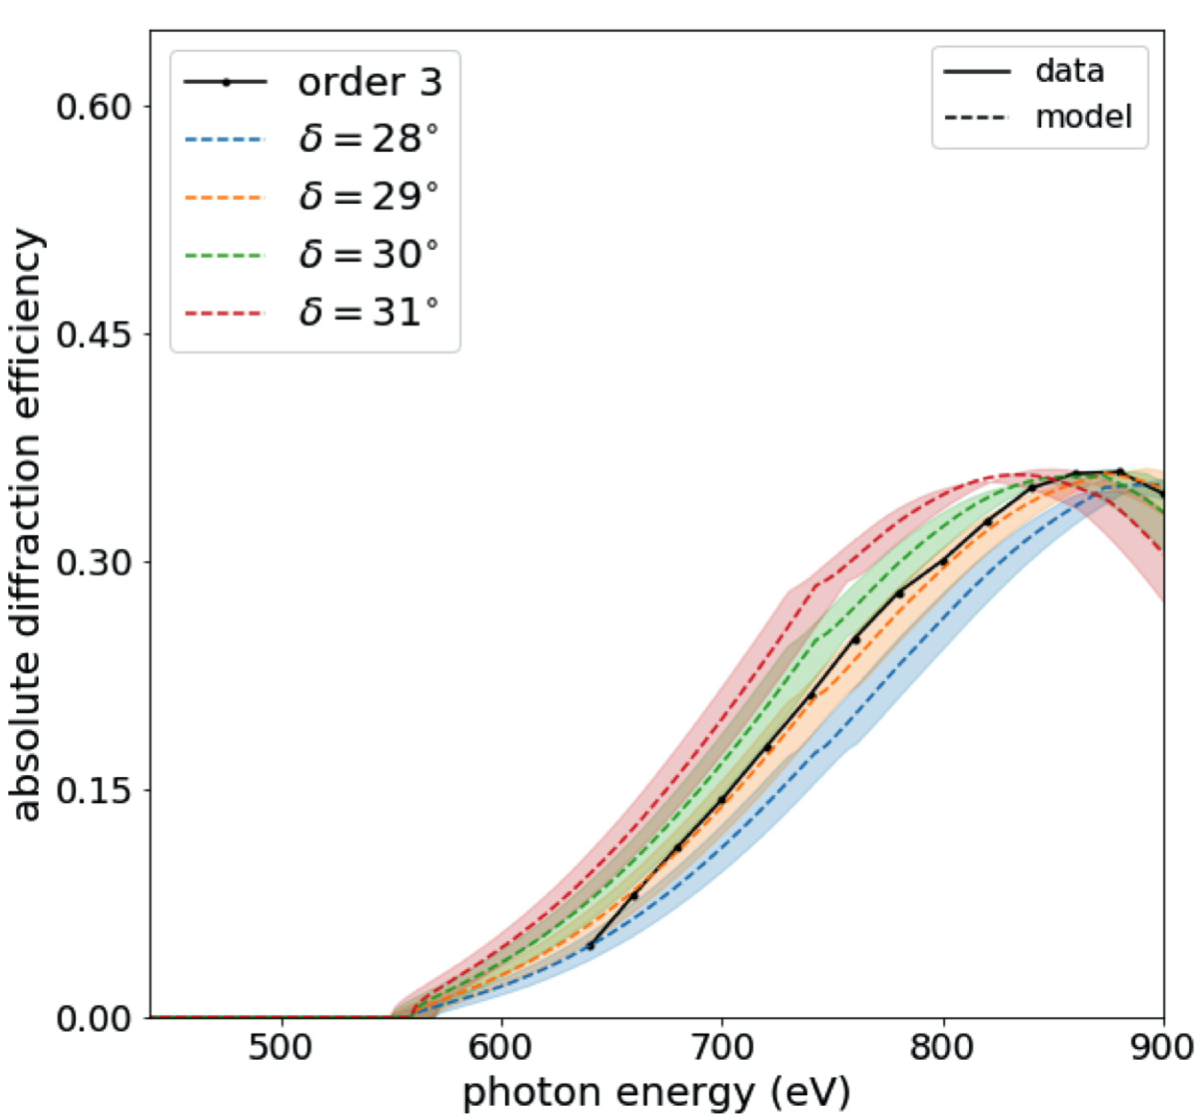
\includegraphics[scale=0.25]{Chapter-4/Figures/si_double2_b.png}
 \caption[Measured absolute diffraction efficiency data in second and third orders for the silicon master compared to \textsc{PCGrate-SX} models of varying blaze angle]{Measured absolute diffraction efficiency data with $n=2$ and $n=3$ for the silicon master compared to \textsc{PCGrate-SX} models with $28^{\circ} \leq \delta \leq 31^{\circ}$, $\alpha = 23.7^{\circ}$, and $\gamma = 1.71 \pm 0.03^{\circ}$ (\emph{shaded swaths}) that are normalized to match the data in terms of peak efficiency. These results indicate that $\delta$ for the silicon master is close to the value of $\delta = 30^{\circ}$ measured by AFM \cite{McCoy20b}.}\label{fig:model_si2} %while the shaded swaths represent the $\pm 0.03^{\circ}$ uncertainty in $\gamma$ [\emph{cf.\@} \cref{fig:model_si1}, \emph{top panel}]
 \end{figure} 
With these centroids also depending directly on $\sin \left( \delta \right)$ by \cref{eq:blaze_wavelength_alt_approx}, a series of models with $28^{\circ} \leq \delta \leq 31^{\circ}$ in steps of $1^{\circ}$ are compared to absolute-efficiency data for $n=2$ and $n=3$ in \cref{fig:model_si2}. 

In all of the models used for \cref{fig:model_si2}, $w = \SI{35}{\nm}$ and $\Delta h = \SI{3}{\nm}$ are fixed while the sawtooth angles vary as $\delta$ and $\bar{\delta} = 180^{\circ} - \theta - \delta$ so that the overall groove depth, $h$, follows from \cref{eq:groove_depth}. 
Moreover, the measured data have been corrected for the absorbing effect of small-scale facet surface roughness using the ratio of Nevot-Croce reflectivity (\emph{i.e.}, \cref{eq:Si_layer_refl} with $\sigma_1 = \sigma_2 = \SI{0.4}{\nm}$~RMS) to Fresnel reflectivity (\emph{i.e.}, \cref{eq:Si_layer_refl} with $\sigma_1 = \sigma_2 \to 0$), at the nominal incidence angle $\zeta = 1.70^{\circ}$ [\emph{cf.\@} \cref{tab:nom_params}]. 
The modeled efficiency in each case, which assumes a perfectly smooth grating boundary, was then normalized to match the peak efficiency of the measured data. 
Additionally, dotted lines represent the nominal model with $\gamma = 1.71^{\circ}$ and $\alpha = 23.7^{\circ}$ while the shaded swaths show the $\pm 0.03^{\circ}$ uncertainty in $\gamma$. 
These results support the expectation that the blaze angle of the silicon master is in the neighborhood of the nominal $\langle 311 \rangle$ value of $\delta = 29.5^{\circ}$ as well as the AFM-measured value of $\delta = 30.0 \pm 0.8^{\circ}$ reported in \cref{sec:grating_fab}. 

\subsection{SCIL Replica}\label{sec:scil_replica_sub}
%%%%%%%%%%%%%%%%%%%%%%%%%%%%%%%%%%%%%%%%%--------------------------------------------------
Knowing that variance in $\alpha$ has a small effect on peak-order centroids for $\alpha \approx \delta$ [\emph{cf.\@} \cref{eq:blaze_wavelength_alt_approx}], two different \textsc{PCGrate-SX} models for the coated SCIL replica are plotted in \cref{fig:model_scil1} and compared to the experimental data [\emph{cf.\@} \cref{fig:abs_eff}, \emph{bottom panel}] using uncertainty swaths for $\gamma$ alone. 
\begin{figure}
 \centering
 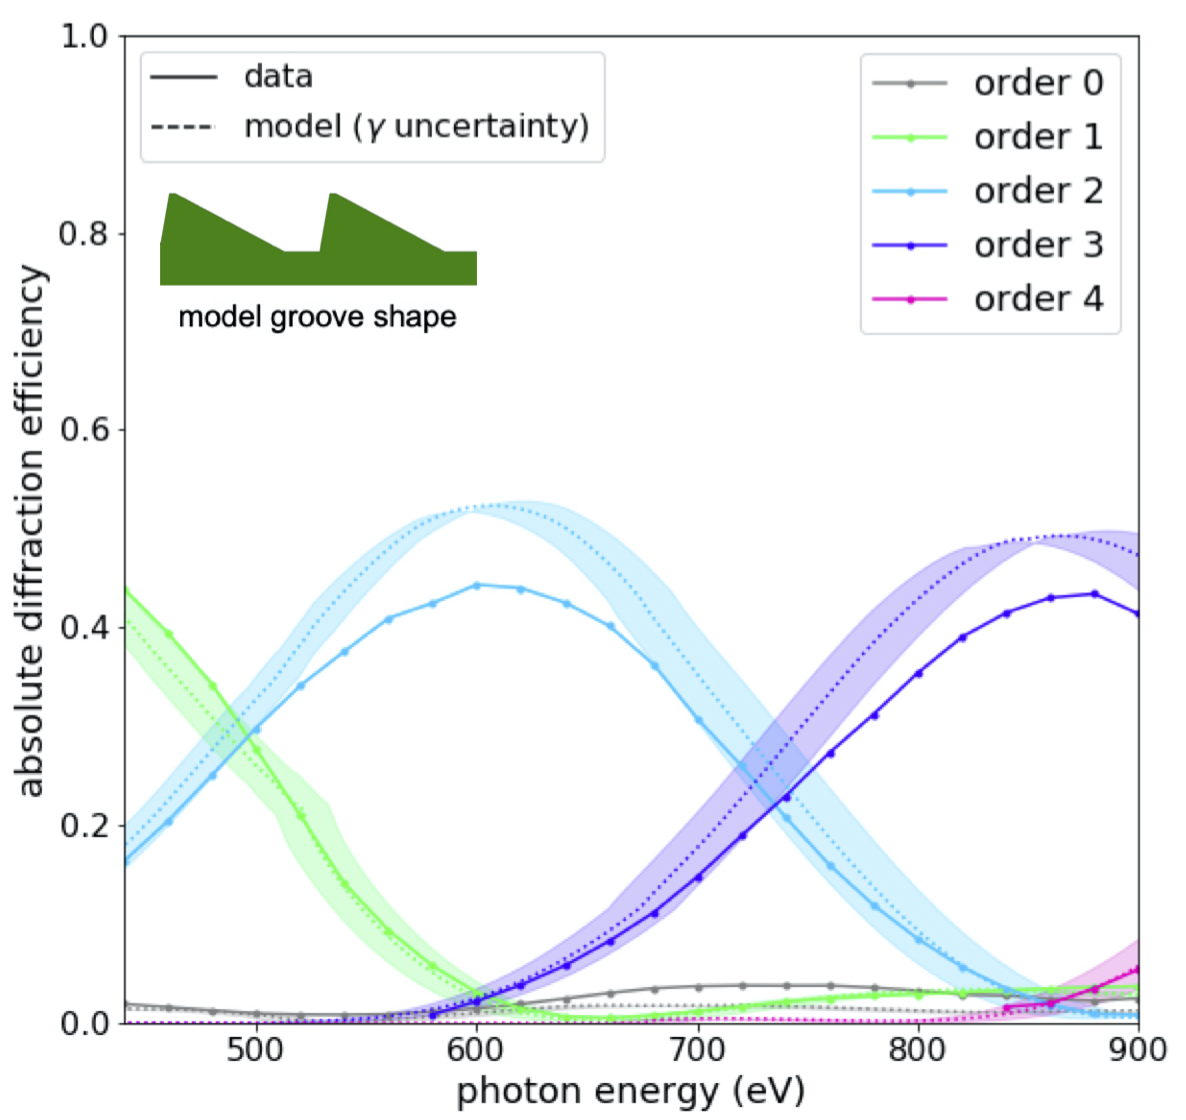
\includegraphics[scale=0.25]{Chapter-4/Figures/scil_double1_a.png}
 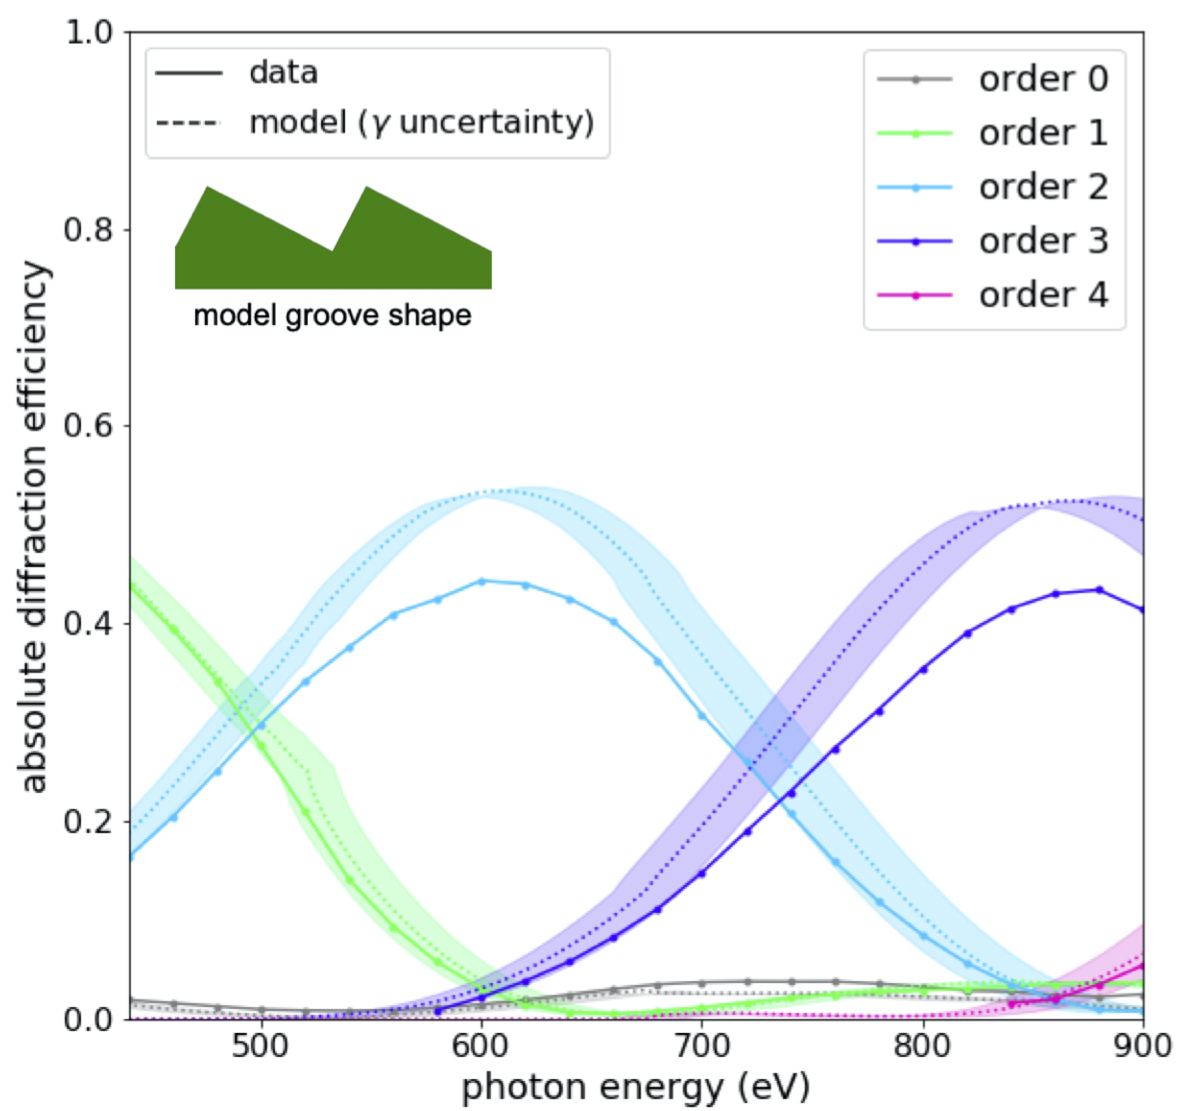
\includegraphics[scale=0.25]{Chapter-4/Figures/scil_double1_b.png}
 \caption[Measured absolute diffraction efficiency data for the coated SCIL replica compared to \textsc{PCGrate-SX} models featuring two different groove shapes, each with a blaze angle of $28^{\circ}$.]{Measured absolute diffraction efficiency data for the coated SCIL replica [\emph{cf.\@} \cref{fig:abs_eff}, \emph{bottom panel}] compared to \textsc{PCGrate-SX} models featuring two different groove shapes, each with $\delta' = 28^{\circ}$, $\alpha = 30.7^{\circ}$ and $\gamma = 1.75 \pm 0.04^{\circ}$ (\emph{shaded swaths}). While the top-panel groove shape more closely resembles the topography of the SCIL replica, it yields model results that are comparable to those produced from the simpler, ideal sawtooth (\emph{bottom panel}) \cite{McCoy20b}.}\label{fig:model_scil1} %The simpler, ideal sawtooth model thus can be used to match predicted peak-order centroids to the measured data.
 \end{figure} 
Both of these models use the nominal values $\gamma = 1.75^{\circ}$ and $\alpha = 30.7^{\circ}$ with $\pm 0.04^{\circ}$ uncertainty in $\gamma$ [\emph{cf.\@} \cref{tab:arc_params}] along with a shrunken blaze angle of $\delta' = 28^{\circ}$, which is an approximate value based on the AFM measurements from \cref{sec:reflectivity}, and specular reflectivity for a gold slab [\emph{cf.\@} \cref{eq:Au_refl}]. 
However, the two models differ in their groove shape details; the model in the top panel of \cref{fig:model_scil1} attempts to emulate the topography of the SCIL replica with a $\bar{\delta} \approx 80^{\circ}$ steep angle, a groove depth of $h' \approx \SI{58}{\nm}$, which was estimated from AFM measurements, a flat-bottom portion of width $w \approx \SI{35}{\nm}$ and a \SI{5}{\nm}-wide flat top so as to approximate a slightly rounded groove apex. 
On the other hand, the model in the bottom panel is taken to be the ideal case of a sawtooth with a sharp, $90^{\circ}$ apex angle and no flat-bottom portion, which is consistent with $h' \approx \SI{66}{\nm}$. 
As is apparent in \cref{fig:model_scil1}, the two models for the SCIL replica yield similar results, where in each case, the centroids of peak orders roughly match the data for $\delta' = 28^{\circ}$ while the overall efficiency in each peak order is over-estimated, even with facet roughness taken into account. 
The primary difference between the two models is that the more detailed groove facet in the top panel predicts slightly lower efficiency in peak orders so as to match the data more closely than does the model that assumes an ideal groove facet. 

With both model variants in \cref{fig:model_scil1} giving nearly-identical results in terms of peak-order centroids, the ideal sawtooth model in the right panel offers more simplicity for analyzing the impact of resist shrinkage due to $\delta'$ essentially being the only free parameter for a fixed grating geometry. 
This latter model therefore can be used to constrain the shrunken blaze angle by comparing the data to several models with varying values for $\delta'$, so long as the models are normalized to match the peaks of the measured data as in \cref{fig:model_si2}. 
\begin{figure}
 \centering
 %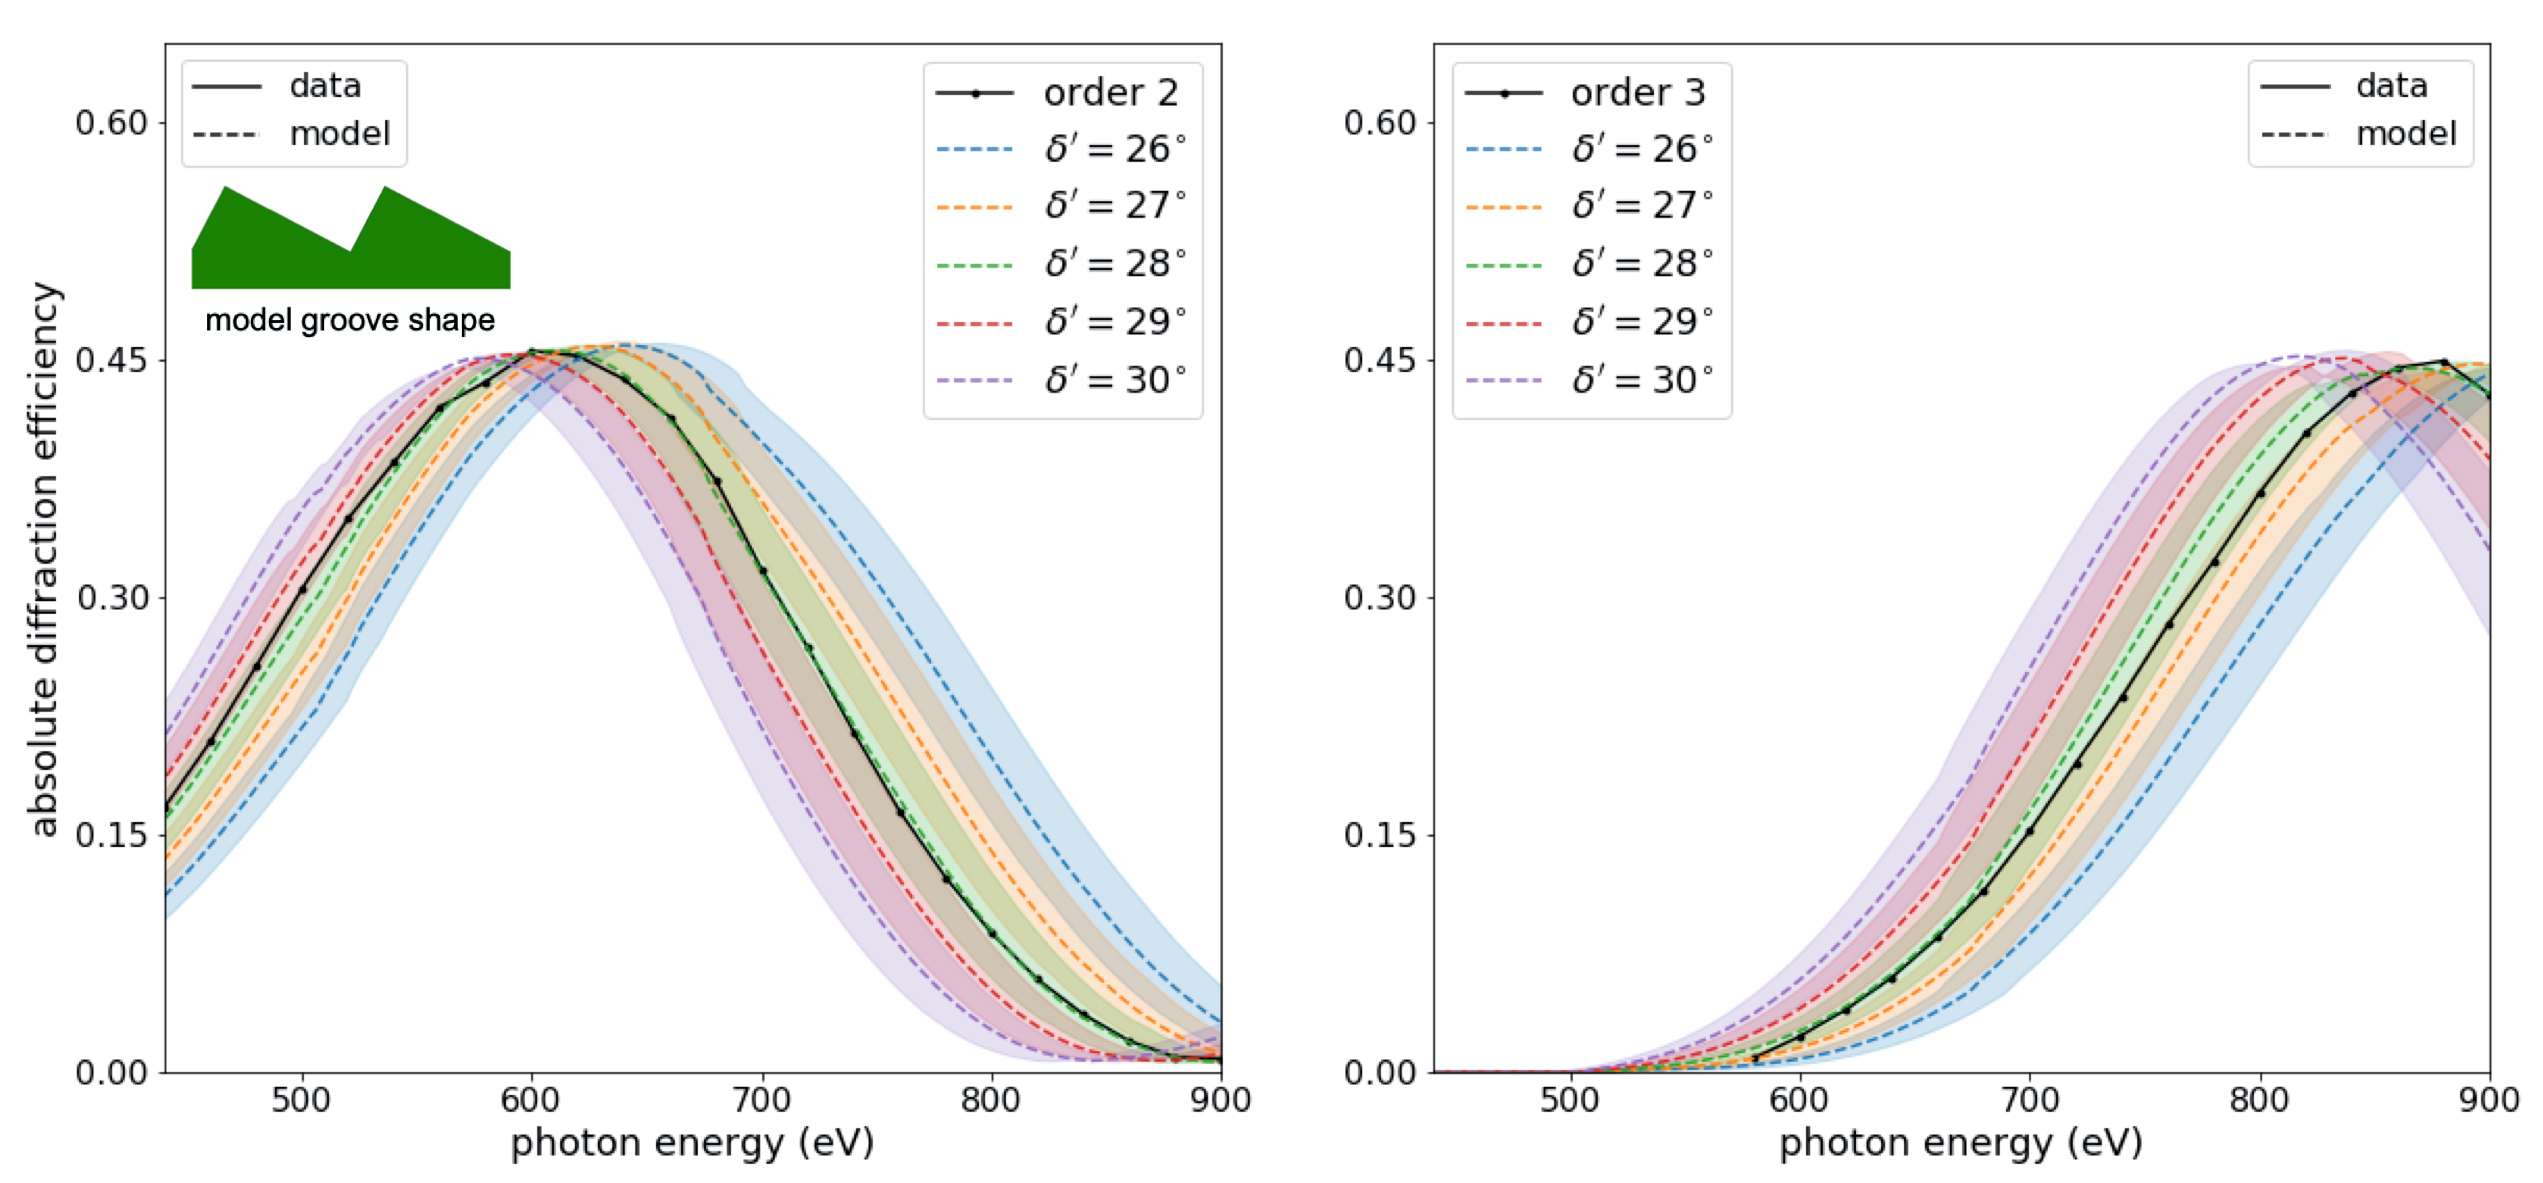
\includegraphics[scale=0.37]{Chapter-4/Figures/scil_double2.pdf}
 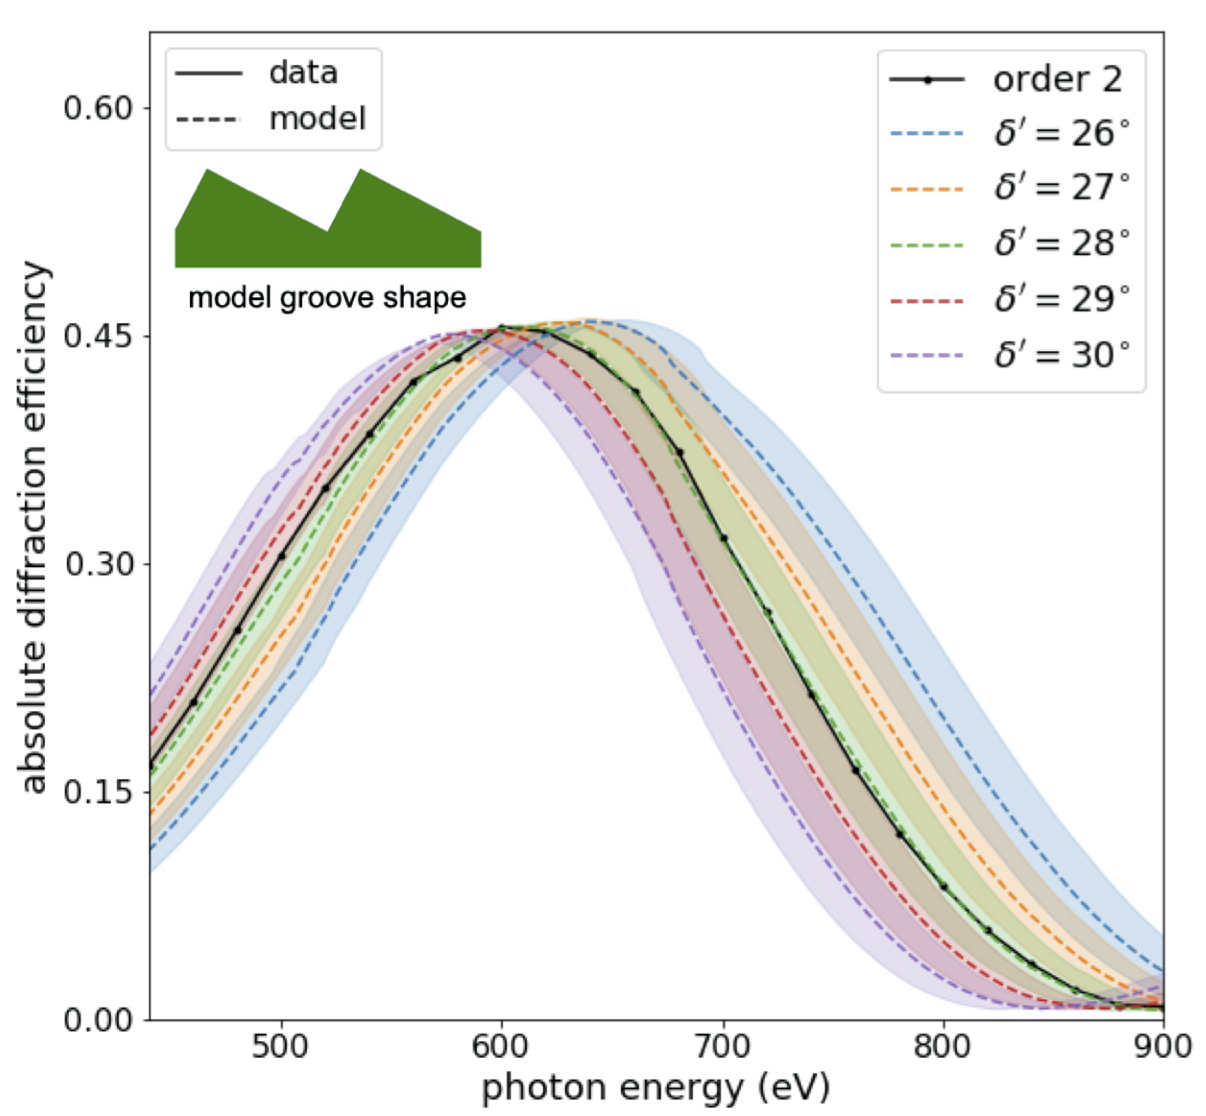
\includegraphics[scale=0.25]{Chapter-4/Figures/scil_double2_a.png}
 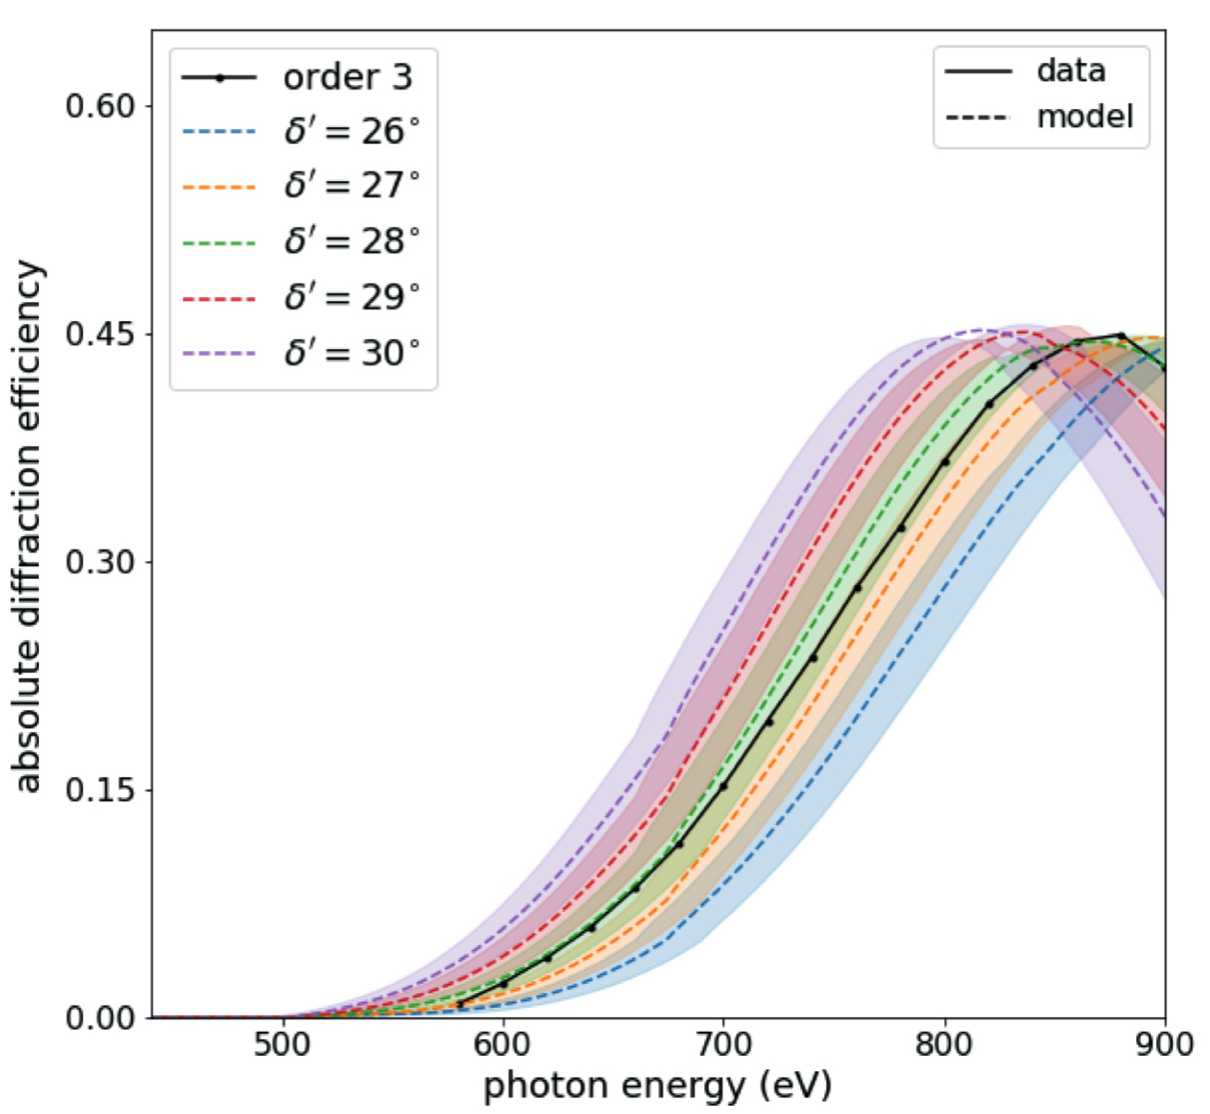
\includegraphics[scale=0.25]{Chapter-4/Figures/scil_double2_b.png}
 \caption[Measured absolute diffraction efficiency data in in second and third orders for the coated SCIL replica compared to \textsc{PCGrate-SX} models that assume an ideal sawtooth with varying blaze angles.]{Measured absolute diffraction efficiency data with $n=2$ and $n=3$ for the coated SCIL replica, corrected for surface roughness using \cref{eq:Au_refl}, and compared to \textsc{PCGrate-SX} models that assume an ideal sawtooth [\emph{cf.\@} \cref{fig:model_scil1}, \emph{bottom panel}] with $26^{\circ} \leq \delta' \leq 30^{\circ}$, $\alpha = 30.7^{\circ}$ and $\gamma = 1.75 \pm 0.04^{\circ}$ (\emph{shaded swaths}), which have been normalized to match the data to show that the measured data most closely match a grating with $\delta' = 28^{\circ}$ \cite{McCoy20b}.}\label{fig:model_scil2} 
 \end{figure} 
This is demonstrated in \cref{fig:model_scil2}, where the absolute diffraction data for the SCIL replica in orders $n=2$ and $n=3$ are each plotted against five \textsc{PCGrate-SX} models with $26^{\circ} \leq \delta' \leq 30^{\circ}$ in steps of $1^{\circ}$, all with $\alpha = 30.7^{\circ}$ and $\gamma = 1.75 \pm 0.04^{\circ}$, the latter of which is represented by uncertainty swaths. 
The data plotted in \cref{fig:model_scil2} have been corrected for surface-roughness losses through division of the Nevot-Croce exponential term in \cref{eq:Au_refl} while the models assume perfectly smooth surfaces and are normalized to the data in terms of peak efficiency. 

From the results presented in \cref{fig:model_scil2}, it is apparent that the measured data are most consistent with the $\delta' = 28^{\circ}$ model, as expected from AFM measurements.  
Although this analysis does not tightly constrain $\delta'$, it does demonstrate that the SCIL replica functions as a blazed grating with a facet angle reduced by $\sim 2^{\circ}$ relative to the silicon master that has been shown to exhibit $\delta \approx 30^{\circ}$. % a blaze angle close to $\delta = 30^{\circ}$. 
\begin{figure}
 \centering
 %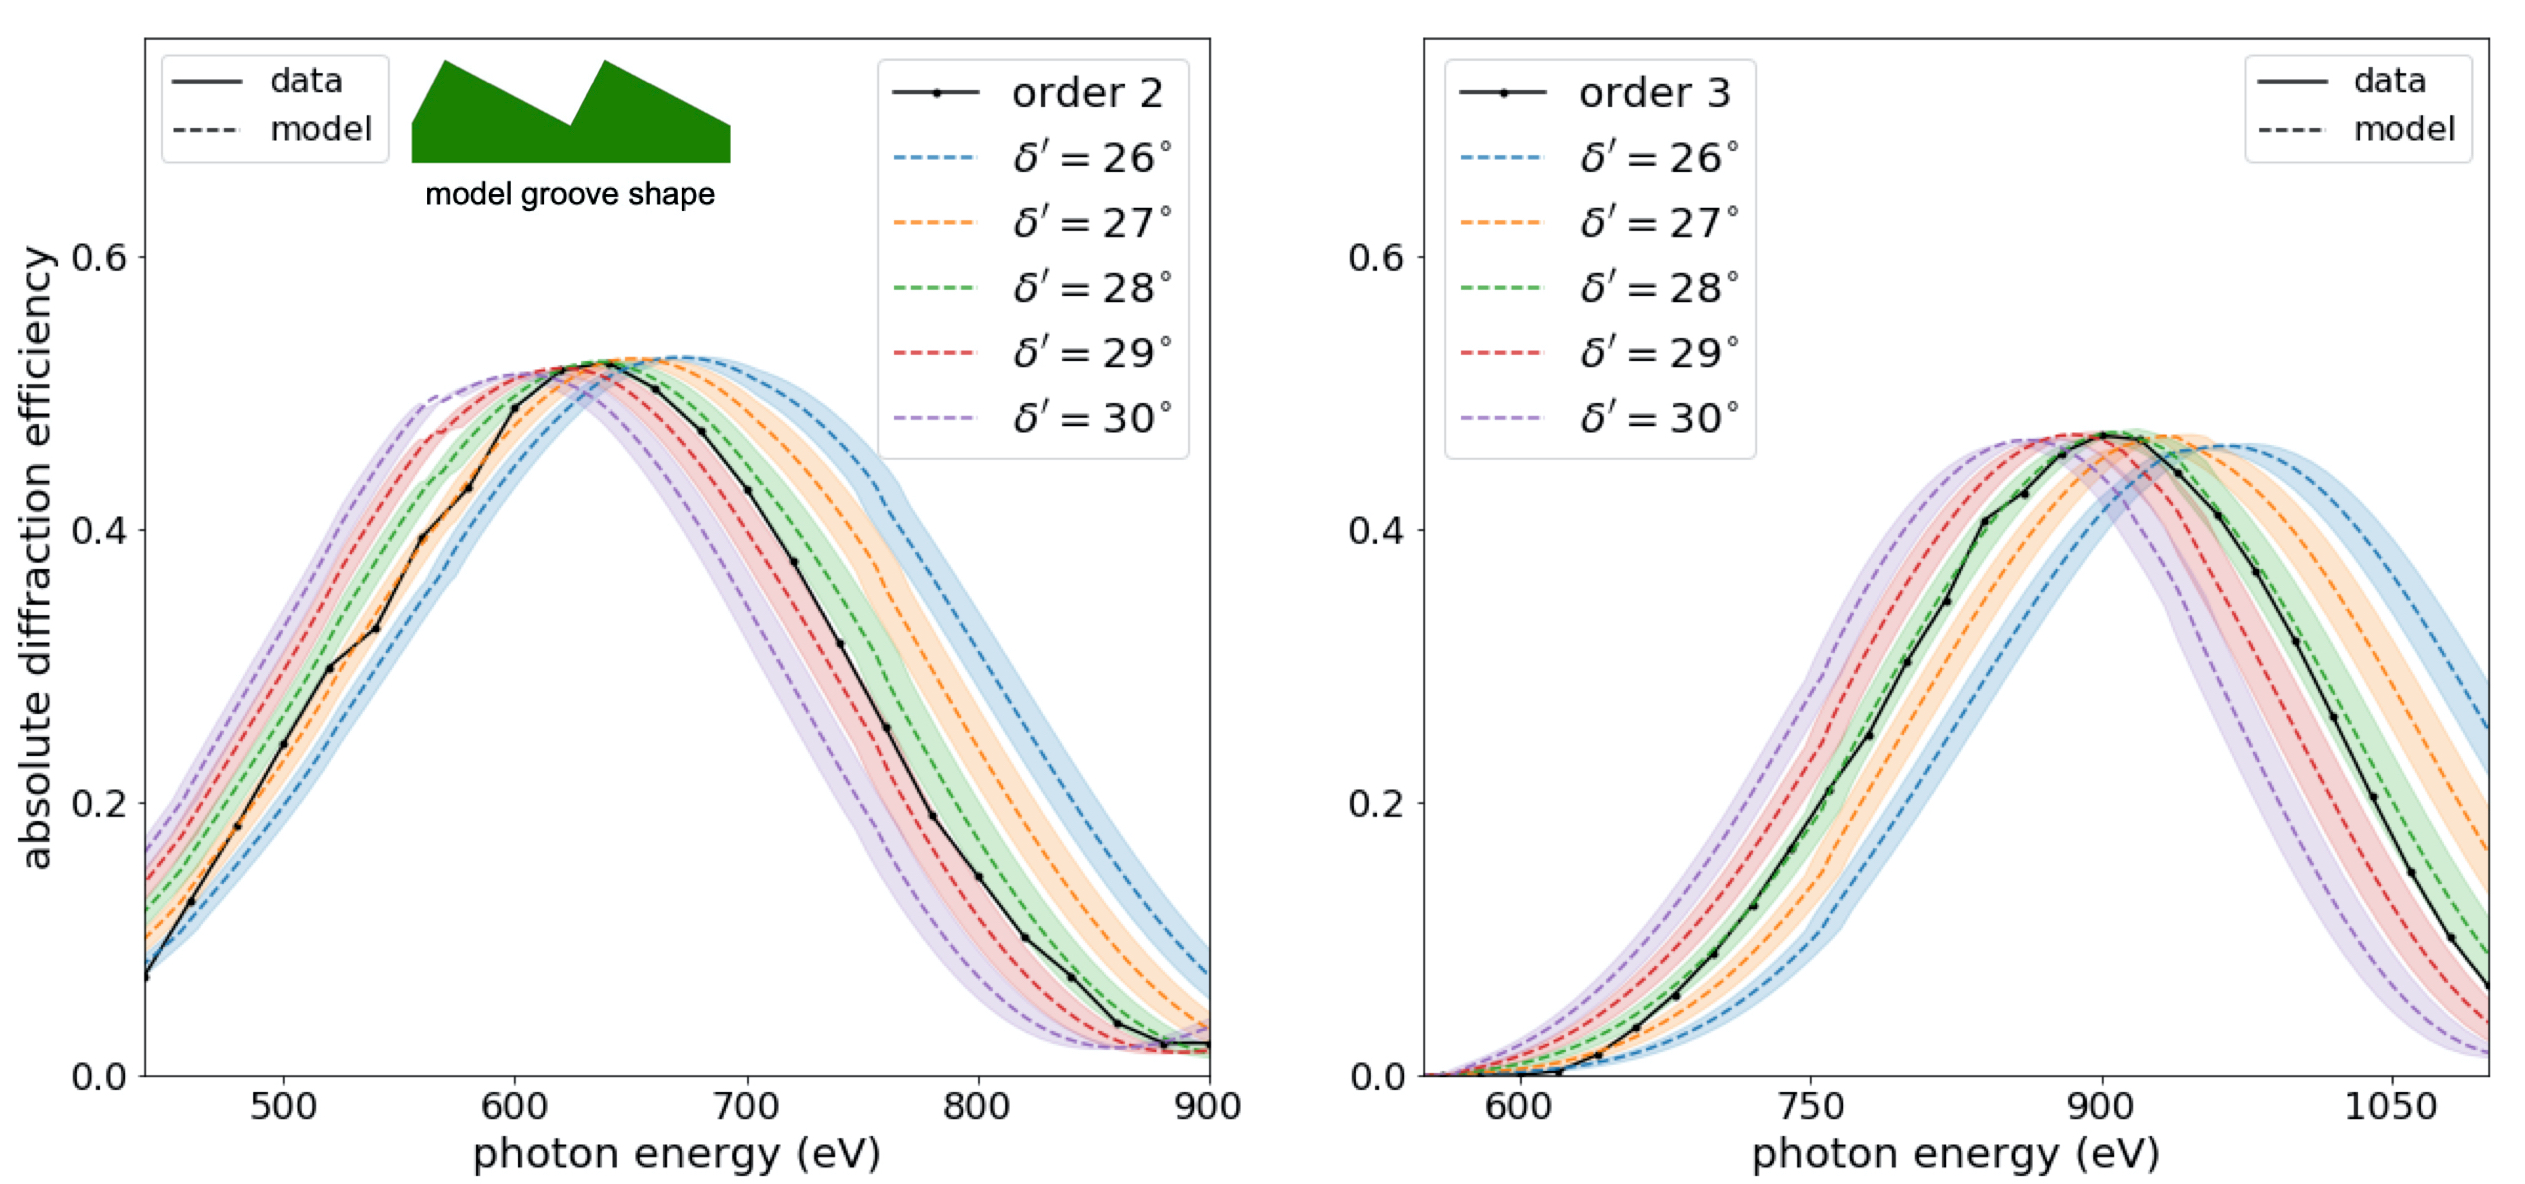
\includegraphics[scale=0.37]{Chapter-4/Figures/uvnil_double.pdf}
 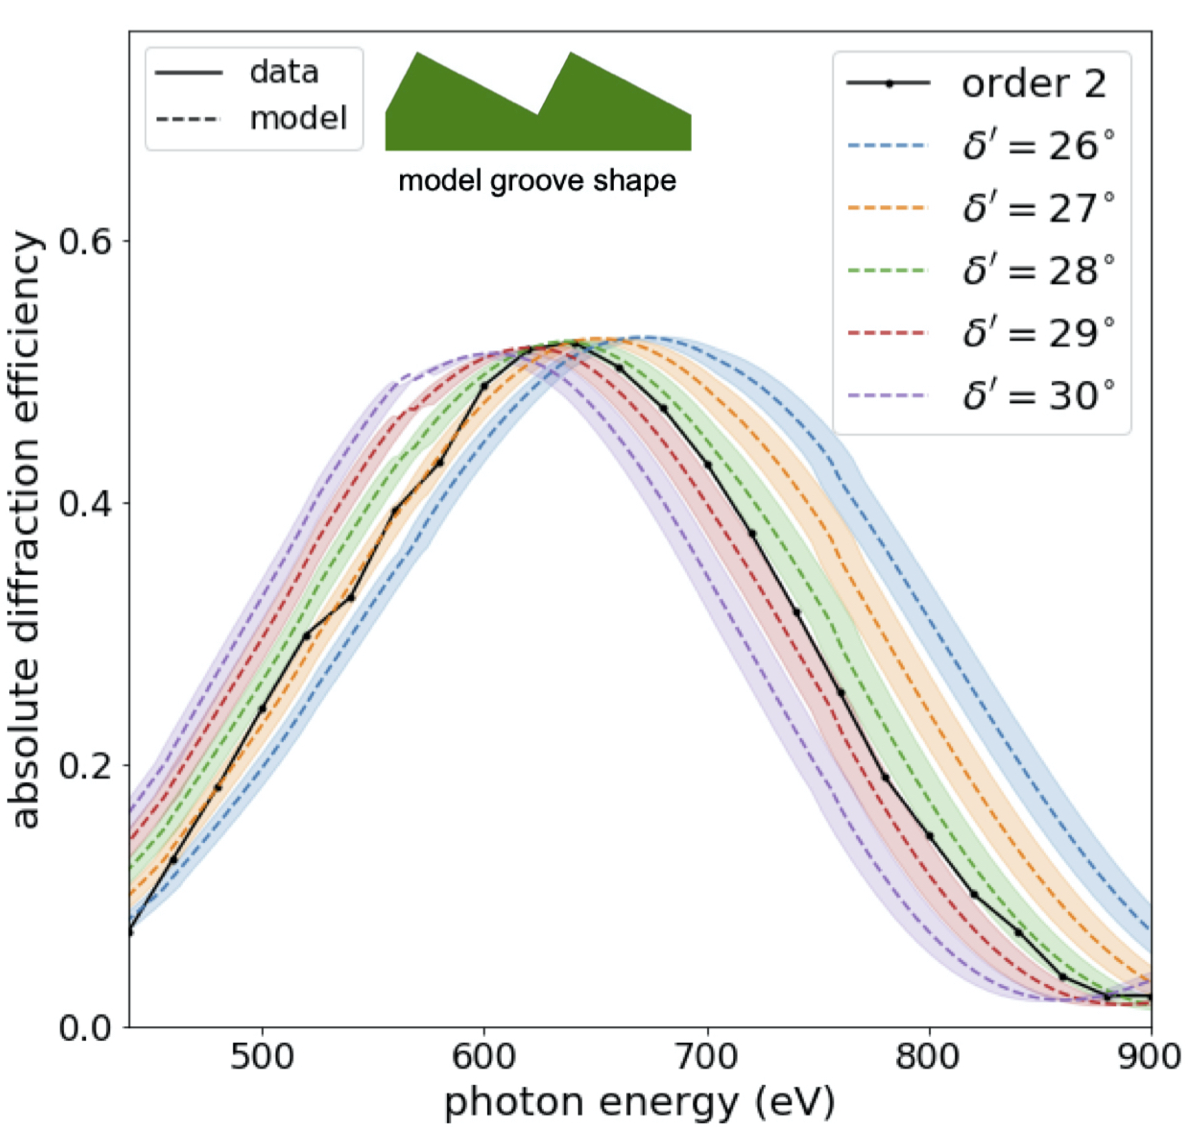
\includegraphics[scale=0.25]{Chapter-4/Figures/uvnil_double_a.png}
 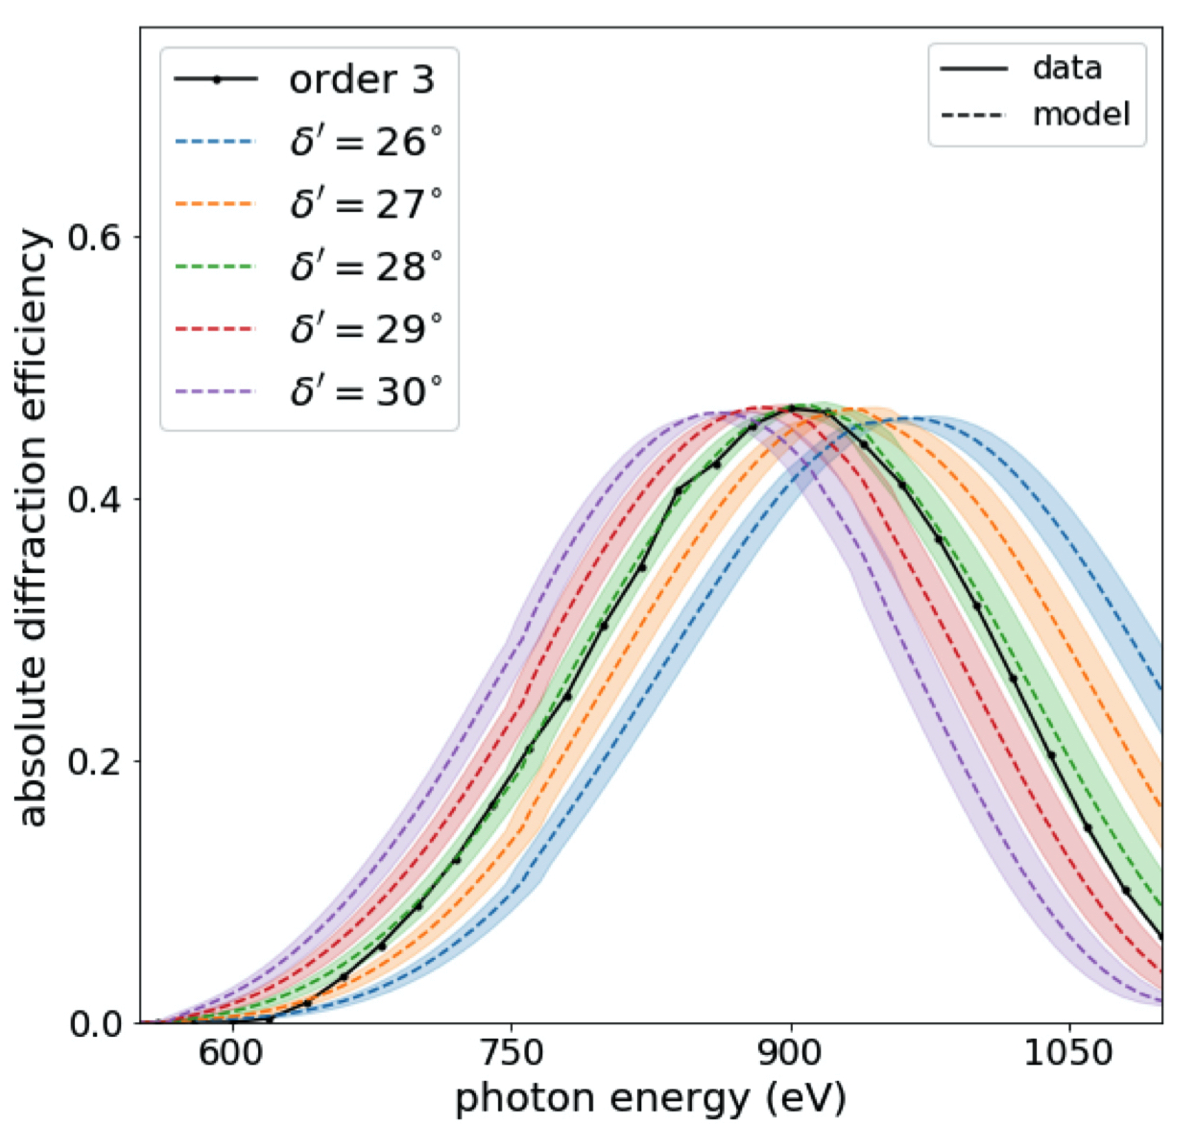
\includegraphics[scale=0.25]{Chapter-4/Figures/uvnil_double_b.png}
 \caption[Measured absolute diffraction efficiency data in second and third orders for a coated UV-NIL replica]{Measured absolute diffraction efficiency data with $n=2$ and $n=3$ for the coated UV-NIL replica \cite{Miles18} compared to \textsc{PCGrate-SX} models that assume an ideal sawtooth [\emph{cf.\@} \cref{fig:model_scil1}, \emph{bottom panel}] with $26^{\circ} \leq \delta' \leq 30^{\circ}$, $\alpha = 24.5^{\circ}$ and $\gamma = 1.66 \pm 0.02^{\circ}$ (\emph{shaded swaths}). As in \cref{fig:model_scil2}, the measured data were corrected for surface roughness using \cref{eq:Au_refl} and normalized to match the data to show that the data most closely match $\delta' = 28^{\circ}$.}\label{fig:model_uvnil} 
 \end{figure} %These results also show that the measured data most closely match a grating with $\delta' = 28^{\circ}$.
This modeling scheme was repeated using the soft x-ray diffraction efficiency data presented by Miles, et~al.~\cite{Miles18}, which were gathered using a gold-coated UV-NIL replica produced from the same silicon master [\emph{cf.\@} \cref{fig:uv_nil_AFM}] in a geometry with $\alpha = 24.5 \pm 1.6^{\circ}$ and $\gamma = 1.66 \pm 0.02^{\circ}$. 
While the shrinkage mechanism for UV-curable resists differs fundamentally from thermodynamically-curable sol-gel resist, these results shown in \cref{fig:model_uvnil} indicate that the measured data also most closely match $\delta' = 28^{\circ}$. 
This suggests that the impact of resist shrinkage in \SI{90}{\celsius}-treated sol-gel resist is comparable to that of standard UV-NIL with $\sim \SI{10}{\percent}$ volumetric shrinkage, as expected from the considerations presented in \cref{sec:grating_fab}. 

\subsection{Geometric Resist-Shrinkage Model}\label{sec:shrinkage_model}
%%%%%%%%%%%%%%%%%%%%%%%%%%%%%%%%%%%%%%%%%--------------------------------------------------
To model the observed reduction in blaze angle between the silicon master and the SCIL replica from \cref{sec:silicon_master_sub,sec:scil_replica_sub} in terms of resist shrinkage, it is first assumed that shrinkage effects in the SCIL stamp can be neglected owing to the high intrinsic cross-link density of X-PDMS \cite[\emph{cf.\@} footnote~\ref{footnote:X-PDMS}]{Verschuuren19}. 
The surface-relief profile of the imprinted blazed grating, before resist shrinkage, then is considered to be composed of a series of groove facets with spacing $d \lessapprox \SI{160}{\nm}$ that resembles the inverse of the silicon master [\emph{cf.\@} \cref{fig:master_grating_profile}]. 
These facets are separated from one another approximately by the distance $w \gtrapprox \SI{30}{\nm}$ defined by the width of flat-tops in the silicon master [\emph{cf.\@} \cref{fig:master_grating_profile}] so that the base of each groove facet has a width $b \approx d - w \lessapprox \SI{130}{\nm}$, which is assumed to be a small enough size scale for material relaxation in sol-gel resist. 
\begin{figure}
 \centering
 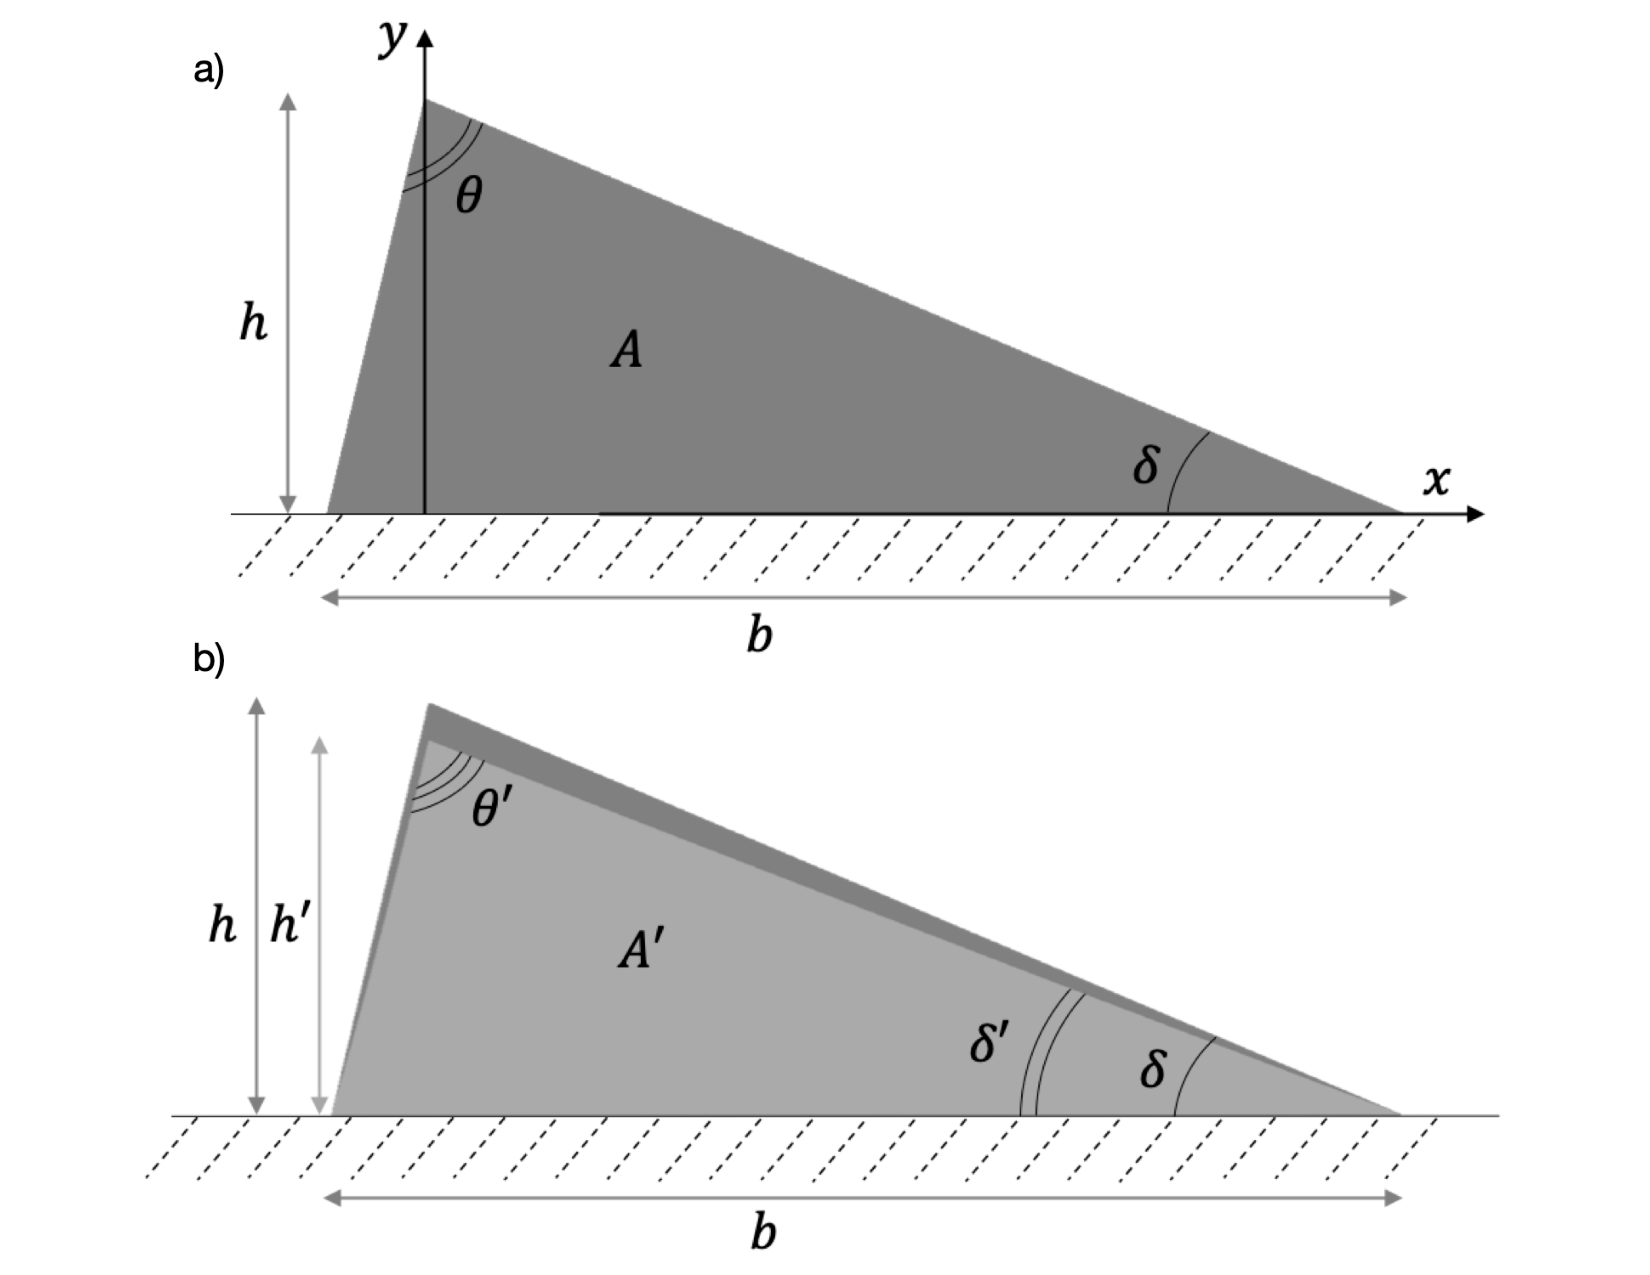
\includegraphics[scale=0.55]{Chapter-4/Figures/shrinkage_model_fig.pdf}
 \caption[Approximate model for resist shrinkage]{Approximate model for resist shrinkage with $y=0$ representing a fixed boundary defined by the residual layer. a) The original facet shape has a blaze angle $\delta = 29.5^{\circ}$, an apex angle $\theta \approx 70.5^{\circ}$ and a cross-sectional area $A = bh/2$. b) A shrunken facet is generated by dividing the original facet shape into \num{1000} layers along the $y$-direction and then requiring that the area of each is reduced by \SI{10}{\percent} with $\chi = 0.1$ and $A'= 0.9 A$ while the ratio between lateral and vertical shrinkage varies as a function of $y$ according to \cref{eq:exp_shrink} for $S$ with $\ell_e / h = 0.05$. The result is reduction in groove depth with $h'/h \approx 0.91$, a steep sidewall featuring slight curvature, an increased apex angle with $\theta' / \theta \approx 1.05$ and crucially, a quasi-flat facet surface with a reduced blaze angle, $\delta' \approx 27.4^{\circ}$ with $\delta' / \delta \approx 0.93$ \cite{McCoy20b}.}\label{fig:shrinkage} 
 \end{figure} 
As illustrated in \cref{fig:shrinkage}(a), it is assumed that the shallow side of the facet takes on the nominal value of $\delta = 29.5^{\circ}$ while the protruding nubs of the master grating then are ignored for simplicity so that the groove depth with $\Delta h = 0$ is $h \lessapprox \SI{67}{\nm}$ by \cref{eq:groove_depth}, where $b/h \approx \cot \left( \delta \right) - \cot \left( \theta + \delta \right) \approx 1.944$ using $\theta \approx 70.5^{\circ}$. 
This angle, $\theta$, which is defined by the crystal structure of silicon [\emph{cf.\@} \cref{fig:master_grating_profile}], serves as the pre-shrinkage apex angle shown in \cref{fig:shrinkage}(a). 

Simulations of resist shrinkage in UV-NIL based on continuum mechanics of elastic media \cite{Shibata10,Horiba_2012} indicate that on average, local volumetric reduction is uniform such that a volume element, $V$, of a continuous medium shrinks to $V'$ given by 
\begin{equation}\label{eq:volume_shrinkage}
 V' = V \left( 1 - \chi \right) ,
 \end{equation}
with $\chi$ as the fractional loss in volume. 
In this regard, the residual layer of resist that exists beneath the groove facets [\emph{cf.\@} \cref{fig:SCIL_SEMs}] is expected to experience reduction in thickness alone such that the initial thickness, $\tau$, reduces to $\tau' = \tau \left( 1 - \chi \right)$ while stress-induced substrate deformation from this laterally-constrained shrinkage is considered to be negligible owing to the \SI{1}{\mm} thickness of the silicon wafer used for the grating replica. 
Each groove facet of the grating profile considered then has a volume given by $V = A \mathcal{L}$, where $A = b h / 2$ is its cross-sectional area and $\mathcal{L}$ is its length. 
Because $\mathcal{L}$ is orders of magnitude larger than the vertical and lateral extents of each groove facet over the \SI{72}{\cm\squared} grating area, however, shrinkage in an imprinted grating is considered to be completely restricted along the grove direction due to the inability of the material network to relax over such a macroscopic size scale. 
The shrunken volume then is given by $V' = A' \mathcal{L}$ so that \cref{eq:volume_shrinkage} reduces to 
\begin{equation}\label{eq:area_shrinkage}
 A' = A \left( 1 - \chi \right) , 
 \end{equation}
where $A'$ is cross-sectional area of a groove facet following resist shrinkage. 
Based on simulations for resist shrinkage in UV-NIL that verify a lack of dependence on residual-layer thickness \cite{Horiba_2012}, it is expected that residual-layer shrinkage does not impact the cross-sectional shape of the groove facets and hence the surface of the residual layer is treated as a fixed boundary. 

The simple resist-shrinkage model formulated here stems from the assumption that throughout each imprinted groove facet, the reduction in cross-sectional area is uniform in magnitude while the ratio of lateral shrinkage to vertical shrinkage varies spatially in a manner consistent with the boundary condition provided by the residual layer. 
This can be expressed by introducing $s_x$ and $s_y$ as functions of position that describe lateral and vertical shrinkage, respectively, so that \cref{eq:area_shrinkage} can be written as 
\begin{subequations}
\begin{equation}\label{eq:area_shrinkage2}
 \frac{A'}{A} = \left( 1 - \chi \right) = \left( 1 - s_x \right) \left( 1 - s_y \right) .
 \end{equation}
Then, defining $S \equiv s_x/s_y$ as the shrinkage aspect ratio, \cref{eq:area_shrinkage2} becomes
\begin{equation}
 \left( 1 - \chi \right) = \left( 1 - S f \right) \left( 1 - f \right) \implies S f^2 - \left( 1 + S \right) f + \chi = 0
 \end{equation}
with $s_x = S f$ and $s_y = f$. 
Considering only $1 \geq S > 0$, this quadratic equation has solutions for $f$ given by 
\begin{equation}\label{eq:quad_solution}
 f = \frac{1 + S - \sqrt{(1+S)^2 - 4 S \chi}}{2 S} ,
 \end{equation}
\end{subequations}
where $f \leq 1$ is ensured so that $A'$ is always positive.  
The fixed boundary provided by the residual layer requires $S = 0$ at $y=0$ so that $s_x = 0$ and $s_y = \chi$ near the base of each groove facet of width $b$. 
On the other hand, $s_x$ should increase from zero as the distance from the boundary increases until ultimately, free shrinkage occurs both laterally and vertically due to the previously-stated assumption that $b \lessapprox \SI{130}{\nm}$ is a small enough size scale for material relaxation in sol-gel resist. 
The shrinkage aspect ratio, $S$, therefore should be a function of $y$ that grows from zero at $y=0$ to a value approaching unity with $s_x = s_y = f = 1 - \sqrt{1 - \chi}$ as $y$ increases toward $h$. 
For the present discussion, this behavior for $0 \leq y \leq h$ is taken to be described approximately by 
\begin{equation}\label{eq:exp_shrink}
 S = 1 - \mathrm{e}^{- y / \ell_e} ,
 \end{equation}
where $\ell_e$, while formally an unknown quantity, is defined as the vertical distance from the boundary at which $S$ reaches $1 - \left( 1 / \mathrm{e} \right) \approx 0.63$. 

The spatially-varying function for $S$ given by \cref{eq:exp_shrink} was incorporated into the resist-shrinkage model by first considering the original groove facet shape shown in \cref{fig:shrinkage}(a) to be composed of \num{1000} rectangular layers, each with an identical, thin, vertical thickness and lateral widths that vary with $y$ so as to emulate a sawtooth with $\delta = 29.5^{\circ}$ and $\bar{\delta} = 180^{\circ} - \theta - \delta \approx 80^{\circ}$ slopes. 
Using \cref{eq:exp_shrink} discretized into \num{1000} $y$ steps for $S$ along with \cref{eq:quad_solution} for $f$, a shrunken facet profile could be produced by requiring the area of each of these layers to be reduced according to $s_x = S f$ and $s_y = f$ for specified values of $\chi$ and $\ell_e$. 
The result in any case is a reduction in groove depth with $h' < h$ while the base of the facet retains its width $b$, causing an increased apex angle, $\theta' > \theta$, and a small level of curvature where $y \lessapprox \ell_e$. 
The active groove facet then flattens to a linear slope as $y$ becomes larger than $\ell_e$ and because of this, the reduced blaze angle, $\delta'$, is extracted from the model by measuring slope only in the upper-half of the facet, where $S \lessapprox 1$ for relatively small values of $\ell_e / h$. 
While the model outputs $h'$ and $\delta'$ are independent from one another, they are related approximately through
\begin{equation}\label{eq:reduced_depth}
 h' \lessapprox \frac{\tan \left( \delta ' \right)}{\tan \left( \delta \right)} h ,
 \end{equation}
but without accurate depth measurements of the silicon master, or any AFM measurements of the composite stamp, it cannot be ruled out that groove-apex rounding during stamp construction and imprint production also contributes to this groove depth reduction. 
Consequently, a measured value for $h'/h$ in this case does not provide a meaningful constraint on resist shrinkage and is not considered further. 
\begin{figure}
 \centering
 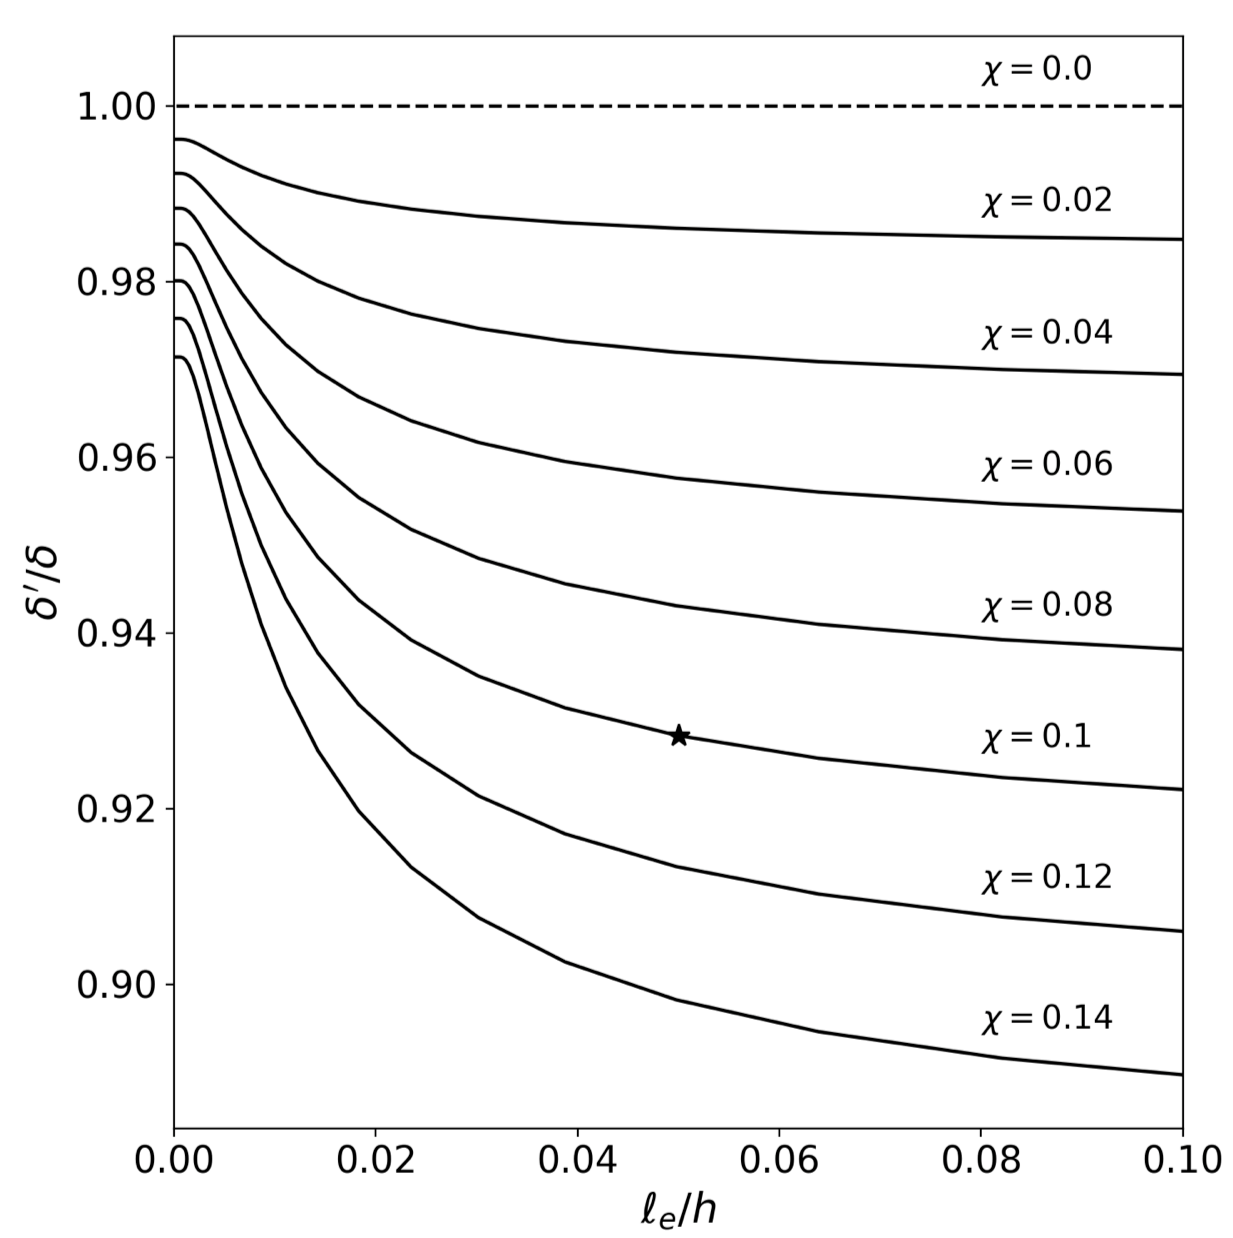
\includegraphics[scale=0.55]{Chapter-4/Figures/shrinkage_blaze_plot_edit.pdf}
 \caption[Reduced blaze angle predicted by the resist-shrinkage model relative to the initial blaze angle as a function of various parameters.]{Reduced blaze angle predicted by the resist-shrinkage model relative to the initial blaze angle, $\delta' / \delta$, as a function of $\ell_e / h$ for various values of $\chi$. With $\chi = 0.1$ and $\ell_e / h = 0.05$ marked by the star, the modeled shrunken facet depicted in \cref{fig:shrinkage} exhibits $\delta' / \delta \approx 0.93$ with $\delta' = 27.4^{\circ}$ and $\delta = 29.5^{\circ}$ \cite{McCoy20b}.}\label{fig:shrinkage_compare} 
 \end{figure}
Similarly, an approximate expression for $\theta'$ depends on $h'$ and $\delta'$:
\begin{equation}
 \cot \left( \theta' \right) \lessapprox \frac{h'}{b} \csc^2 \left( \delta' \right) - \cot \left( \delta' \right)
 \end{equation}
but this parameter is also not constrained experimentally in the present study. 

Predicted values for $\delta' / \delta$ are plotted as a function of $\ell_e / h$ for various values of $\chi$ in \cref{fig:shrinkage_compare}, where the marked star indicates the inputs used for the shrunken facet depicted in \cref{fig:shrinkage}(b). 
Despite $\ell_e / h$ remaining poorly constrained without measurements for $h'/h$ and $\theta' / \theta$, the comparison between the resist-shrinkage model just presented and $\delta' / \delta \approx 0.93$ determined from diffraction-efficiency analysis along with AFM measurements supports the hypothesis stated in \cref{sec:grating_fab} that the level of volumetric shrinkage for a $T_{\text{cure}} = \SI{90}{\celsius}$-treated sol-gel imprint is approximately \SI{10}{\percent}.  
Although this analysis does not tightly constrain $\delta'$, it does demonstrate that the SCIL replica functions as a blazed grating with a facet angle reduced by $\sim 2^{\circ}$ relative to the silicon master, which has been shown to exhibit a blaze angle of $\delta \approx 30^{\circ}$, giving a value for $\delta' / \delta$ that is consistent with a typical shrunken facet with $\chi \approx 0.1$. 
The outputs from this illustrated model using $\chi = 0.1$ and $\ell_e / h = 0.05$ as inputs are $h' \approx 0.91 h$, $\theta' \approx 74.1^{\circ}$ and $\delta' \approx 27.4^{\circ}$ with $\delta' / \delta \approx 0.93$ relative to the assumed initial blaze angle.\footnote{While these models were formulated assuming $\delta = 29.5^{\circ}$, the quantity $\delta' / \delta$ scales approximately with choice of $\delta$.} 

\section{Summary and Conclusions}\label{sec:conclusion}
%%%%%%%%%%%%%%%%%%%%%%%%%%%%%%%%%%%%%%%%%--------------------------------------------------
This chapter describes a SCIL fabrication process for a blazed-grating surface relief imprinted in \textsc{NanoGlass T1100}, a thermodynamically-curable silica sol-gel resist, and the subsequent soft x-ray diffraction-efficiency testing of the grating in an extreme off-plane mount after it was sputter-coated with a thin layer of gold for reflectivity using chromium as an adhesion layer. 
%Although a few diffracted orders were missed systemically during data collection at beamline 6.3.2 of the ALS, 
The collected peak-order efficiency measurements are comparable to previous results obtained for a UV-NIL replica coated with the same material and produced from the same master template, which was fabricated through a process centering on EBL and crystallographic etching in $\langle 311 \rangle$-oriented silicon \cite[\emph{cf.\@} \cref{sec:crystal_etching}]{Miles18}. 
Further analysis that consists of matching theoretical models to measured data shows that while this silicon master yields diffraction efficiency results that are close to a nominal $\langle 311 \rangle$ blaze angle with $\delta \approx 30^{\circ}$, the response of the coated SCIL replica is consistent with a reduced blaze angle of $\delta' \approx 28^{\circ}$, which is the same approximate result obtained for the corresponding UV-NIL replica \cite[\emph{cf.\@} \cref{sec:nanoimprint}]{Miles18}. 
This supports the hypothesis that the replicated grating, which was treated with a $T_{\text{cure}} = \SI{90}{\celsius}$ bake following stamp separation, experienced volumetric shrinkage in the sol-gel resist on the level of \SI{10}{\percent} to provide a blaze angle reduced by $\sim \SI{7}{\percent}$ to give $\delta - \delta' \approx 2^{\circ}$ for $\delta \approx 30^{\circ}$.  
While this result could be better constrained through further diffraction-efficiency testing and more rigorous modeling for resist shrinkage,
it serves as experimental evidence for resist shrinkage in SCIL impacting the performance of a reflection grating in terms of its ability to maximize diffraction efficiency for a specific diffracted angle, $\beta = 2 \delta - \alpha$. 
This is of particular relevance to instrument development for astrophysical soft x-ray spectroscopy that relies on the production of large numbers of identical gratings \cite{Miles19b,Tutt18,McEntaffer19}. 
The impact of resist shrinkage therefore should be compensated for in the fabrication of the master grating to ensure that grating replicas perform as expected. 